\documentclass[12pt]{article}
\usepackage{graphicx}
\usepackage[a4paper, margin=1.8cm]{geometry}
\usepackage{tikz}
\usepackage{times}
\usepackage{tocloft}
\usepackage{titlesec}
\usepackage{array}
\usepackage{tabularx}
\usepackage[table,xcdraw]{xcolor}
\usepackage{caption}
\usepackage{float}
\usepackage{amsmath}
\usepackage[numbers]{natbib}
\bibliographystyle{plainnat}
\usepackage{url}
\usepackage{etoolbox}
\usepackage{adjustbox}
\usepackage{placeins}
\usepackage{booktabs}
\usepackage{subcaption}

% Fix the spacing issue in bibliography
\makeatletter
\patchcmd{\BR@citenum}
  {\begingroup}
  {\itemsep=0pt \parskip=0pt \begingroup}
  {}{}
\makeatother

\renewcommand{\cftsecleader}{\cftdotfill{\cftdotsep}}
% Change the figure and table numbering style
\renewcommand{\thefigure}{\arabic{figure}}
\renewcommand{\thetable}{\arabic{table}}

% Update the table of contents settings
\renewcommand{\cftfigpresnum}{Figure~}
\renewcommand{\cfttabpresnum}{Table~}

% Add spacing between the number and title in the list of figures/tables
\renewcommand{\cftfignumwidth}{5em} 
\renewcommand{\cfttabnumwidth}{4em} 

\captionsetup{font=small, labelfont=bf, labelsep=period}
\newcolumntype{Y}{>{\centering\arraybackslash}X}

\begin{document}
\begin{titlepage}
    \begin{tikzpicture}[remember picture, overlay]
        \draw[line width=1pt, black] ([shift={(10mm, -10mm)}]current page.north west) rectangle ([shift={(-10mm, 10mm)}]current page.south east);
    \end{tikzpicture}
    \centering
    \vspace*{1cm}

    \large
    UNIVERSITY OF SCIENCE AND TECHNOLOGY OF HANOI\\

    \Large
    \textbf{UNDERGRADUATE SCHOOL}

    \vspace{1.5cm}

    
\includegraphics[width=0.9\textwidth]{usth.png}

    \vspace{1.5cm}

    {\Large \textbf{Research and Development}}\\

    \vspace{0.5cm}

    {\Huge \textbf{BACHELOR THESIS}}

    \vspace{2cm}

    By\\
    \vspace{0.5cm}
    \Large ``\textbf{NGUYEN SON (BI12-389)}''\\
    \Large Information and Communication Technology
    \vfill
    Title\\
    \vspace{0.5cm}
    {\LARGE ``\textbf{Utilizing Pose Estimation in \\Physical Enhancement Gaming Application}''}

    \vspace{2cm}

    \begin{tabular}{@{}l@{}}
        External Supervisor: Prof. Nguyen Duc Dung - IOIT/VAST \\
        Internal Supervisor: Dr. Kieu Quoc Viet - ICTLab/USTH
    \end{tabular}
    \vfill
    \normalsize{\textit{Hanoi, July 2024}}

\end{titlepage}


% Table of Contents Page
\pagenumbering{roman}
\tableofcontents
\clearpage

% Acknowledgements
\section*{Acknowledgements}
\addcontentsline{toc}{section}{ACKNOWLEDGEMENTS}
\hspace*{1.5em}First and foremost, I would like to express my deepest gratitude to Professor Nguyen Duc Dung from IOIT/VAST, who has provided invaluable support and guidance as my external supervisor throughout this project. 
Despite Game Production not being his area of expertise, he has offered extensive assistance and thoughtful feedback on my Internship Thesis. Professor Dung's insightful comments and constructive criticism have also significantly influenced the direction of this project. His encouragement and confidence in my abilities have been a constant source of motivation, particularly during the most challenging periods. I am deeply appreciative of the considerable time he has devoted to reviewing my work, providing detailed feedback, and engaging in discussions on new ideas. I feel fortunate to have had the opportunity to work with such a dedicated and knowledgeable mentor.\\

I would like to extend my sincere gratitude to Mr. Kieu Quoc Viet, my internal supervisor, for his ongoing support and valuable guidance. I appreciate his kind and approachable nature, which has made our conversation enjoyable as always. His advice and encouragement have been extremely valuable especially when it comes to thesis writing. His knowledge has greatly improved the clarity and structure of my work.\\

Special thanks go to Miss Le Thi Bich Phuong for her exceptional teaching sessions on Model Building in Blender. Her expertise and patience in explaining concepts for a newbie in Graphic Design like me have been incredibly helpful. The skills I have acquired under her guidance have played a crucial role in bringing my project to life.\\

I would like to thank my friends for their valuable time and feedback during the play-testing of my game. Their helpful comments have significantly contributed to its development. Moreover, their unwavering support and belief in me and my project have been a constant source of motivation, helping me to persevere and stay dedicated to this endeavor.\\

Finally, I want to say my most sincere thanks to my family for their endless love and support throughout this journey. Their encouragement and compassion have given me the motivation and strength to overcome challenges and obstacles to pursue my academic goals.
\clearpage

% List of Abbreviations
\section*{List of Abbreviations}
\addcontentsline{toc}{section}{LIST OF ABBREVIATIONS}
\renewcommand{\arraystretch}{1.5}
\vspace{0.2cm}
\begin{tabular}{@{} >{\bfseries\raggedleft\arraybackslash}p{0.3\textwidth} p{0.7\textwidth}@{}}
    API  & Application Programming Interface          \\
    CNN  & Convolutional Neural Network               \\
    CPU  & Central Processing Unit                    \\
    DDR  & Dance Dance Revolution                     \\
    FPS  & Frame Per Second                           \\
    GPU  & Graphics Processing Unit                   \\
    ICT  & Information and Communication Technology   \\
    IOIT & Institute of Information Technology        \\
    IP   & Internet Protocol                          \\
    JPG  & Joint Photographic Experts Group           \\
    JSON & JavaScript Object Notation                 \\
    PC   & Personal Computer                          \\
    PCK  & Percentage of Correct Keypoints            \\
    RAM  & Random Access Memory                       \\
    RGB  & Red Green Blue                             \\
    ROI  & Region of Interest                         \\
    TCP  & Transmission Control Protocol              \\
    TXT  & Text File                                  \\
    USTH & University of Science and Technology Hanoi \\
    VAST & Vietnam Academy of Science and Technology  \\
\end{tabular}
\clearpage

% List of Tables
\listoftables
\addcontentsline{toc}{section}{LIST OF TABLES}
\clearpage

% List of Figures
\listoffigures
\addcontentsline{toc}{section}{LIST OF FIGURES}
\clearpage

% Acknowledgements
\section*{Abstract}
\addcontentsline{toc}{section}{ABSTRACT}
This thesis presents the development of "Aller! USTH," a video game designed for gamers seeking fitness through the use of pose estimation models. 
The game aims to fix the problem of sedentary lifestyles among students and young adults, which can lead to serious health problems. 
"Aller! USTH" features various gameplay modes, such as endless-running, object-slicing, and shape-fitting, all of which require players to do physical movements. 
These movements are captured by a laptop or PC webcam and processed using pose estimation models like MediaPipe and MoveNet to understand and reflect the player's actions in the game. 
Evaluations were taken on the models using metrics such as Percentage of Correct Keypoints (PCK), accuracy, and precision. 
The overall game performance was based through FPS and response time tests, as well as a beta launch to gather user feedback on the game experience.
\clearpage

% Introduction
\pagenumbering{arabic}
\section{INTRODUCTION}
\subsection{Context and Motivation}
\hspace*{1.5em}In today's digital age, video games have become a popular form of entertainment for students and young adults. They can captivate players for hours with their engaging experiences.
However, this wave of video games in popularity does come with a downside. Many people, especially students and young adults, are spending too much time playing games and not enough time doing any form of physical activity. 
This sedentary lifestyle will resulted serious consequences for our health in the long run.\\

According to the University of Southern California (2023), adults spend around 9.5 hours each day being sedentary. 
Being inactivity for that long may caused serious consequences, like increasing the risk of developing chronic diseases such as diabetes, heart disease, and even certain cancers \cite{usc2023}.
Futhermore, The American Heart Association (AHA) highlighted that regular physical activity is needed to maintain good health. They recommend that adults engage in at least 150 minutes of moderate exercise per week \cite{aha2017}. This can help lower the risks compares to a total sedentary lifestyle and can promote overall well-being.\\

Another survey by the National Instututes of Health (2022) shows that 70\% of gamers do physical activity fewer than two days per week \cite{klasnja2022}. This is really worth concerning, especially considering that the number of gamers worldwide keep growing everyday.
According to Newzoo's Global Games Market Report, the number of gamers is expected to reach more than 3.38 billion in 2024 \cite{wijman2023}. This trend highlights the urgent need for innovative solutions that can somehow merges physical activity with gaming activities, to promoting a healthier lifestyle for gamers while still keeping them entertained.\\

Top health organizations, like the Centers for Disease Control and Prevention (CDC) and World Health Organization (WHO), have warning us about the dangers of sitting too much for the longest time.
According to the CDC, nowadays young adult's sedentary lifestyles increases the risk of premature death from all causes, no matters how much excercise or work out was done to make up after that \cite{carlson2018}. This again really shows the importance of addressing sedentary behavior as a separate health risk factor.
The WHO has launched several initiatives to combat physical inactivity, including the Global Action Plan on Physical Activity 2018-2030. This plan aims to reduce physical inactivity by 15\% by 2030, highlighting the need for collective action to promote physical activity and reduce sedentary behavior \cite{who2017}.\\

The gaming industry itself is also getting ready for more active gaming experiences flooding the gaming market. For example, games like Wii Fit and Just Dance have shown that combine entertainment with physical activity can still attract gamers from any experience level to try and be entertained in long-term.
However, these games often need specialized equipment like a remote or censor camera..., which can be a really big barrier to widespread the game's good intention. This asked for the need for more accessible solutions that can easily merges physical activity into popular gaming formats, making it more enjoyable for gamers to get moving without paying a huge price.
There is a clear opportunity for innovation in the gaming industry to develop solutions that promote physical activity, without requiring specialized equipment. By doing so, the industry can help to reduce sedentary behavior and promote a healthier lifestyle for gamers worldwide.\\

\subsection{Objectives}
\hspace*{1.5em}Recognizing the pressing issue of sedentary behavior among gamers, particularly within the University of Science and Technology of Hanoi (USTH), this thesis aims to develop an innovative solution.
The primary objective of this thesis is to create "Aller! USTH," a video game that integrates physical activity with gameplay using human pose estimation technology. The game is designed to motivate players to engage in physical movements while playing, promoting a healthier lifestyle.

\begin{itemize}
    \item Create a engaging game inspired by popular games like Subway Surfers, Fruit Ninja, and Hole in the Wall, to appeal to a broad audience.
    \item Utilize human pose estimation technology to track and incorporate players' physical movements into the game mechanics, requiring players to perform specific physical actions to progress.
    \item Encourage regular physical activity among players, addressing the issue of sedentary behavior prevalent among gamers, particularly students and young adults.
    \item Shift gaming habits towards more active and health-conscious practices, demonstrating that gaming can be both fun and beneficial for physical health.
\end{itemize}

\subsection{Proposed Outcomes}
\hspace*{1.5em}This thesis aims to achieve two primary outcomes.

\begin{enumerate}
    \item Develop "Aller! USTH," a functional and engaging game that effectively merges physical activity with gaming using human pose estimation technology. This ensures players perform specific physical movements to advance in the game.
    \item Demonstrate the game's ability to integrate physical activity into gameplay and its potential to reduce sedentary behavior by making exercise a part of daily gaming routines.
\end{enumerate}

\subsection{Thesis Structure}
This thesis is organized into seven main chapters, each focusing on different aspects of the development and evaluation of the ``Aller! USTH'' game:

\begin{itemize}
    \item \textbf{Introduction}: Provides the context and motivation behind the development of ``Aller! USTH'', outlines the objectives of the project, and the proposed outcomes.
    \item \textbf{Related Works}: Reviews existing literature and projects related to active gaming and pose estimation technologies, highlighting their strengths and weaknesses.
    \item \textbf{Project Implementation}: Details the steps taken to develop ``Aller! USTH'', including the project pipeline, timeline, and technologies implemented.
    \item \textbf{Model}: Describes the data collection and preprocessing methods, the architecture of the pose estimation models used, and the evaluation metrics.
    \item \textbf{Game Design}: Outlines the design aspects of ``Aller! USTH'', including game modes, level design, controls, gameplay, and other key aspects.
    \item \textbf{Testing / Experimental Validation}: Focuses on the testing and validation of the game, detailing the methods used to assess its effectiveness in promoting physical activity and the results obtained.
    \item \textbf{Summary}: Provides a summary of the findings, conclusions drawn from the development and testing of ``Aller! USTH'', and suggestions for future development to further enhance the game’s impact on physical activity and health.
\end{itemize}

\clearpage


\section{RELATED WORKS}

\subsection{Related Work Analysis}
The concept of merging physical activity with gaming is not new, and several attempts have been made in the past with varying degrees of success. Here, we delve into notable examples in the market: Wii Sports, Kinect Sports, RingFit Adventure, and Dance Dance Revolution (DDR), examining their technologies, gameplay mechanics, pros, and cons.

\subsubsection{Wii Sports}
Developed and published by Nintendo, Wii Sports was released in 2006 as a launch title for the Wii console. The game utilizes motion sensors embedded in the Wii Remote to track player movements, detecting motion and rotation to translate physical actions into on-screen movements. The game includes various sports such as tennis, bowling, golf, baseball, and boxing, each requiring different physical movements, providing a diverse range of activities. Wii Sports introduced a revolutionary way for casual gamers to interact with video games, encouraging physical activity through engaging sports simulations. Its intuitive controls and family-friendly appeal made it accessible to a broad audience, promoting a more active form of gameplay \cite{wiisports2007}.
\begin{itemize}
\item \textbf{Pros}: Wii Sports introduced casual gamers to a new way of interacting with games; encouraged some level of physical activity.
\item \textbf{Cons}: The level of activity is often minimal, with many games not requiring significant movement beyond wrist actions. Studies have suggested that while Wii Sports can increase activity levels, it's not enough to meet recommended exercise guidelines \cite{sherbal2020}.
\end{itemize}
\begin{figure}[ht]
\centering

\includegraphics[width=0.3\textwidth]{logo-wii.png}
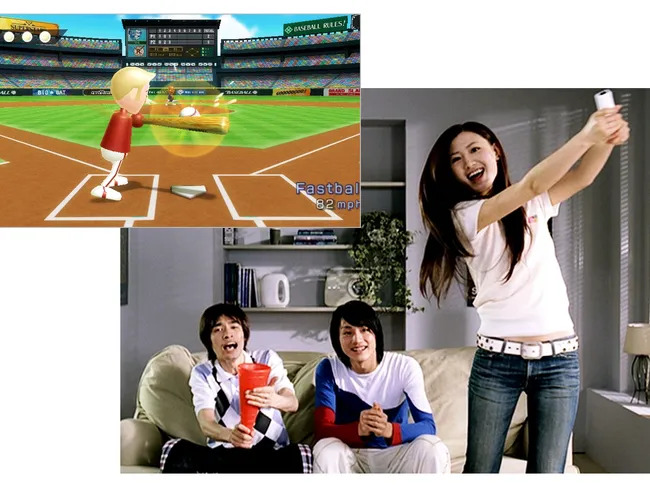
\includegraphics[width=0.45\textwidth]{Market-Wii.jpg}
\caption{Wii Sports: Logo (left) and Gameplay (right).}
\end{figure}

\subsubsection{Kinect Sports}
Developed by Rare and published by Microsoft Studios, Kinect Sports was released in 2014 for the Xbox One. The game uses the Microsoft Kinect camera to track the entire body's movements, employing depth-sensing technology and advanced algorithms to capture full-body motion and enable a wide range of physical interactions. Players engage in various sports and physical activities, including soccer, rock climbing, tennis, bowling, and target shooting. The game encourages full-body movement, making it a more immersive and physically engaging experience. The game’s use of full-body tracking technology allows for a more dynamic range of physical activities and provides a fun, family-friendly experience that promotes physical movement \cite{kinect2013}.
\begin{itemize}
\item \textbf{Pros}: Encourages full-body movement and provides a fun, family-friendly experience.
\item \textbf{Cons}: Limited in its scope and depth, often seen more as a novelty than a serious exercise or gaming tool \cite{zhang2012}.
\end{itemize}
\begin{figure}[ht]
\centering

\includegraphics[width=0.3\textwidth]{logo-kinect.jpg}
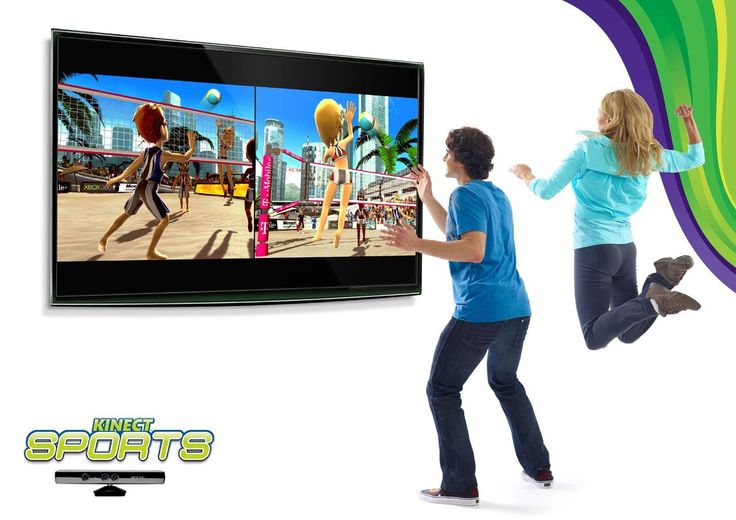
\includegraphics[width=0.45\textwidth]{Market-Kinect.jpg}
\caption{Kinect Sports : Logo (left) and Gameplay (right).}
\end{figure}

\subsubsection{RingFit Adventure}
Developed and published by Nintendo, RingFit Adventure was released in 2019 for the Nintendo Switch. The game combines a physical resistance ring (Ring-Con) and a leg strap with motion sensors to track the player’s activity. These peripherals are used to perform various exercises, which are then translated into in-game actions. Players navigate an adventure game by performing physical exercises such as jogging in place, squats, and overhead presses. The game’s narrative and role-playing elements make exercising more engaging and entertaining. RingFit Adventure has been well-received for its innovative approach to making exercise fun and engaging. The combination of an adventure game narrative with physical exercises creates a compelling fitness experience that can motivate players to stay active \cite{ring2021}.
\begin{itemize}
\item \textbf{Pros}: Well-received for making exercise fun and engaging with an adventure game narrative \cite{jiang2022}.
\item \textbf{Cons}: Requires the purchase of specific hardware and might not appeal to hardcore gamers accustomed to traditional gaming experiences.
\end{itemize}
\begin{figure}[ht]
\centering

\includegraphics[width=0.3\textwidth]{logo-ring.jpg}
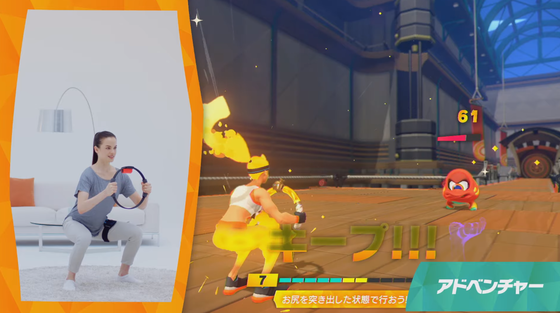
\includegraphics[width=0.45\textwidth]{market-ring.png}
\caption{RingFit Adventure: Logo (left) and Gameplay (right).}
\end{figure}

\subsubsection{Dance Dance Revolution (DDR)}
Developed by Konami, Dance Dance Revolution (DDR) was first released in 1998 and has since become a staple in both arcades and home gaming setups. The game uses a dance mat equipped with pressure sensors to detect foot placement. Players step on the mat's arrows in sync with music and on-screen prompts, creating a dance-like experience. The game features various songs and difficulty levels, challenging players to improve their coordination and rhythm. DDR promotes vigorous physical activity and has been used in fitness regimes and school physical education programs. It offers a fun way to engage in cardiovascular exercise, improving players’ fitness levels while providing entertainment \cite{ddr2017}.
\begin{itemize}
\item \textbf{Pros}: Promotes vigorous physical activity and has been used in fitness regimes and school physical education programs.
\item \textbf{Cons}: Limited to dance moves and requires a dedicated space and setup.
\end{itemize}
\begin{figure}[h]
\centering

\includegraphics[width=0.35\textwidth]{logo-ddr.jpg}
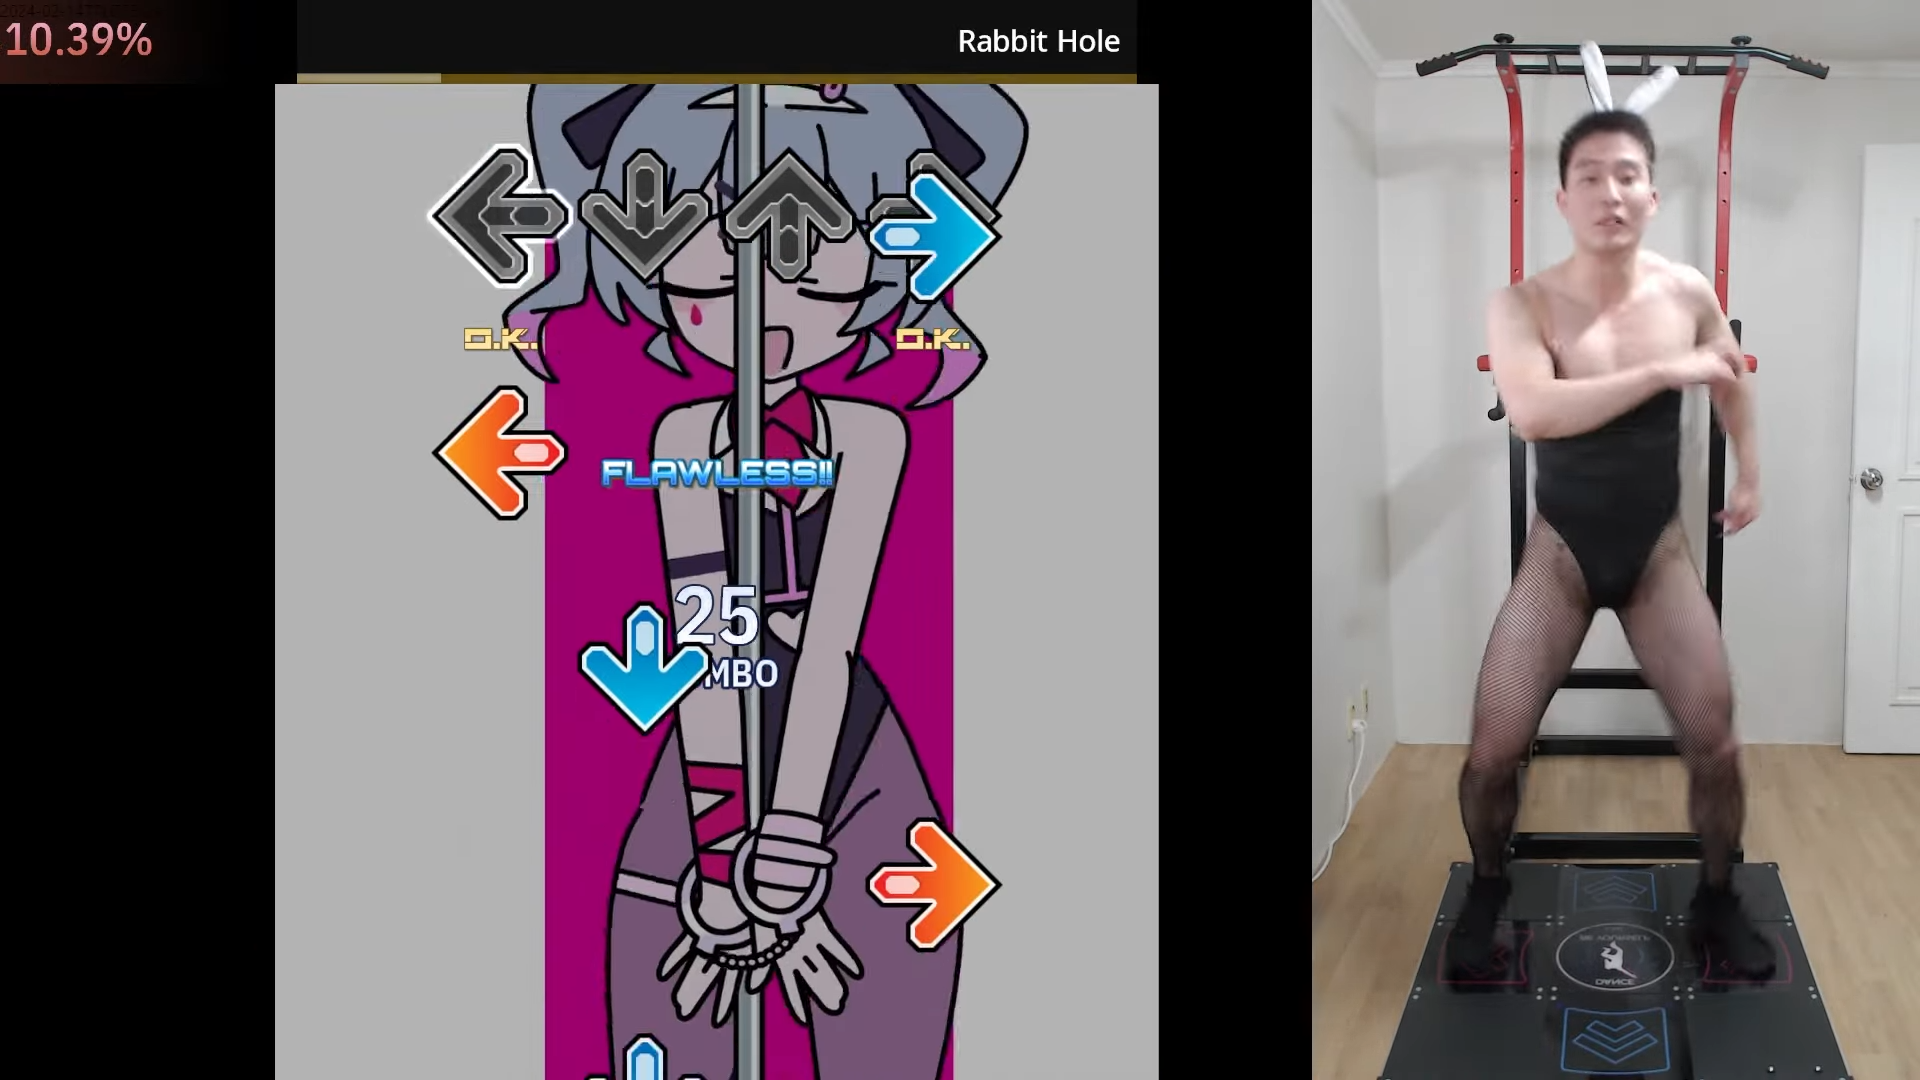
\includegraphics[width=0.5\textwidth]{market-ddr.png}
\caption{DDR: Logo (left) and Gameplay (right).}
\end{figure}

\subsection{Key Insights}
\hspace*{1.5em}To ensure the success of Aller! USTH, it is essential to learn from the strengths and weaknesses of existing active video games.
By analyzing their pros and cons, we can identify key features and improvements to incorporate into Aller! USTH.\\

One critical aspect to emulate from games like Wii Sports and Kinect Sports  is the level of engagement and accessibility. These games introduced casual gamers to a new way of interacting with games through intuitive controls and engaging gameplay, making them accessible to a broad audience. To capture this engagement, Aller! USTH should implement intuitive controls and design a game that is both family-friendly and accessible to a wide range of players.\\

A significant drawback of Wii Sports and similar games is the minimal physical activity required, often limited to wrist movements, which does not provide substantial health benefits. To avoid this, Aller! USTH should ensure that the game demands significant physical movement that meets recommended exercise guidelines, offering real health benefits. Incorporating full-body tracking, as seen in Kinect Sports , can provide an immersive and physically engaging experience, encouraging players to be more active.\\

Games like RingFit Adventure and DDR have shown the effectiveness of combining physical exercises with vigorous activity. RingFit Adventure successfully made exercising fun and motivating by integrating physical exercises with engaging gameplay mechanics. DDR promotes vigorous physical activity and provides an effective cardiovascular workout. Aller! USTH can benefit from these examples by combining physical exercises with engaging and diverse gameplay mechanics. Additionally, designing the game to offer a variety of physical movements and vigorous activity will help improve players' fitness levels.\\

One of the common cons observed in games like Kinect Sports  and RingFit Adventure is the reliance on specific hardware, which can be a barrier to entry. Aller! USTH should aim to minimize the need for specific hardware, making the game more accessible to a broader audience. Furthermore, while DDR is limited to dance moves and requires a dedicated space, Aller! USTH should ensure that the game can be played in a typical home environment without excessive space or setup requirements. This approach will make the game more practical and appealing to users.\\

By taking the best ideas from other active games and addressing their weaknesses, we can create a game that's both fun and effective at promoting physical activity. That's the goal of Aller! USTH - to make exercise feel like a game, and to help players develop healthy habits that will last a lifetime.\\

% \newgeometry{left=0.1cm, right=0.1cm}

\begin{table}[H]
    \centering
    \caption{Market Competition.}
    \rowcolors{2}{gray!25}{white}
    \begin{tabularx}{\textwidth}{|>{\columncolor{gray!50}}Y|Y|Y|Y|Y|Y|}
        \hline
        \textbf{Competitors}        & \textbf{Wii Sports}           & \textbf{Kinect Sport } & \textbf{RingFit Adventure}   & \textbf{Dance Dance Revolution} & \textbf{Aller! USTH}           \\
        \hline
        \textbf{Technology}         & Motion Ssensors in Wii Remote & Kinect camera                & Resistance Ring \& Leg Strap & Dance mat with Pressure Sensors & Webcam \& Pose Detector        \\
        \hline
        \textbf{Type of Activity}   & Various sports                & Full-body movement           & Adventure-based Exercise     & Rhythmic Stepping               & Varied Full-body Movement      \\
        \hline
        \textbf{Hardware Required}  & Wii Remote \& console         & Kinect \& console            & Ring-Con \& Leg Strap        & Dance Mat \& Console            & Standard Webcam \&  PC/Laptop  \\
        \hline
        \textbf{Engagement Level}   & Casual                        & Moderate                     & High                         & High                            & High                           \\
        \hline
        \textbf{Physical Intensity} & Low to Moderate               & Moderate                     & Moderate to High             & High                            & Moderate to High               \\
        \hline
        \textbf{Long-term Appeal}   & Low to Moderate               & Low                          & Moderate                     & Moderate to High                & High                           \\
        \hline
        \textbf{Accessibility}      & Requires Console \& Remote    & Requires Kinect \& console   & Requires Additional Hardware & Requires Mat \& Space           & High (uses existing  hardware) \\
        \hline
        \textbf{Target Audience}    & Casual Gamers \&  Families    & Casual Gamers \&  Families   & Casual Gamers \&  Families   & Hardcore Gamers                 & Gamers seeking Fitness         \\
        \hline
    \end{tabularx}
\end{table}

% \restoregeometry
\clearpage
\section{PROJECT IMPLEMENTATION}
\subsection{Project Pipeline}
\hspace*{1.5em}Here is the short version of the project pipeline: 
\begin{figure}[h]
    \centering
    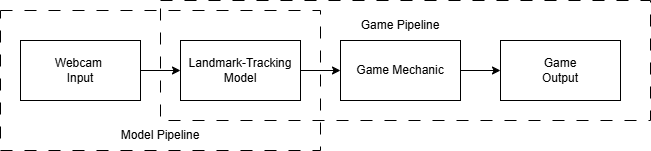
\includegraphics[width=1\textwidth]{short.drawio.png}
    \caption{Short Workflow.}
\end{figure}

As illustrated in the pipeline diagram, the project workflow starts by capturing real-time video input from the laptop or PC webcam. This input is processed using a Landmark-Tracking or Pose Detection Model in Python, which analyzes the player's movements and generates an array of keypoints representing their pose. These keypoints are then sent to Unity, where the game mechanics are implemented using C\#. The game logic interprets these keypoints to control the in-game character's actions, ensuring that the player's physical movements are accurately reflected in the game. Finally, this processed input results in real-time game output, where the in-game character responds to the player's movements, providing an interactive and engaging gaming experience that promotes physical activity.

\subsection{Project Timeline}
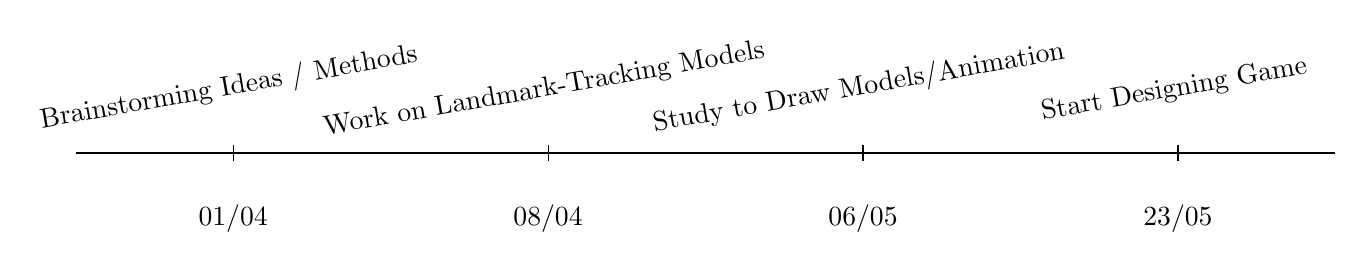
\begin{tikzpicture}
    \draw (0,0) -- (16,0);
    
    \foreach \x in {2,6,10,14}
    \draw (\x cm,3pt) -- (\x cm,-3pt);
    
    \draw (2,0) node[below=15pt] {01/04} node[above=15pt, rotate=10] {Brainstorming Ideas / Methods};
    \draw (6,0) node[below=15pt] {08/04} node[above=15pt, rotate=10] {Work on Landmark-Tracking Models};
    \draw (10,0) node[below=15pt] {06/05} node[above=15pt, rotate=10] {Study to Draw Models/Animation};
    \draw (14,0) node[below=15pt] {23/05} node[above=15pt, rotate=10] {Start Designing Game};
\end{tikzpicture}

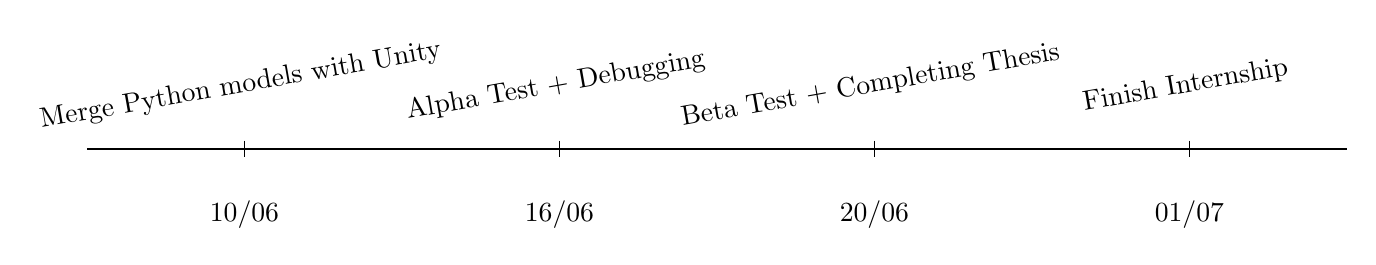
\begin{tikzpicture}
    \draw (0,0) -- (16,0);
    
    \foreach \x in {2,6,10,14}
    \draw (\x cm,3pt) -- (\x cm,-3pt);
    
    \draw (2,0) node[below=15pt] {10/06} node[above=15pt, rotate=10] {Merge Python models with Unity};
    \draw (6,0) node[below=15pt] {16/06} node[above=15pt, rotate=10] {Alpha Test + Debugging};
    \draw (10,0) node[below=15pt] {20/06} node[above=15pt, rotate=10] {Beta Test + Completing Thesis};
    \draw (14,0) node[below=15pt] {01/07} node[above=15pt, rotate=10] {Finish Internship};
\end{tikzpicture}

\clearpage
\subsection{Technology Implemented}
\subsubsection{Graphic Design}
Blender is chosen for this project's 3D graphic design application because it's free, open-source, and constantly updated by a large community. All of the player's skeleton model, skin, and every small object of the game and even all of the hallways were built here. However, animating models manually in Blender doesn't work in Unity, so Mixamo's was used for the pre-made skeleton animations.
\begin{figure}[ht]
    \centering
    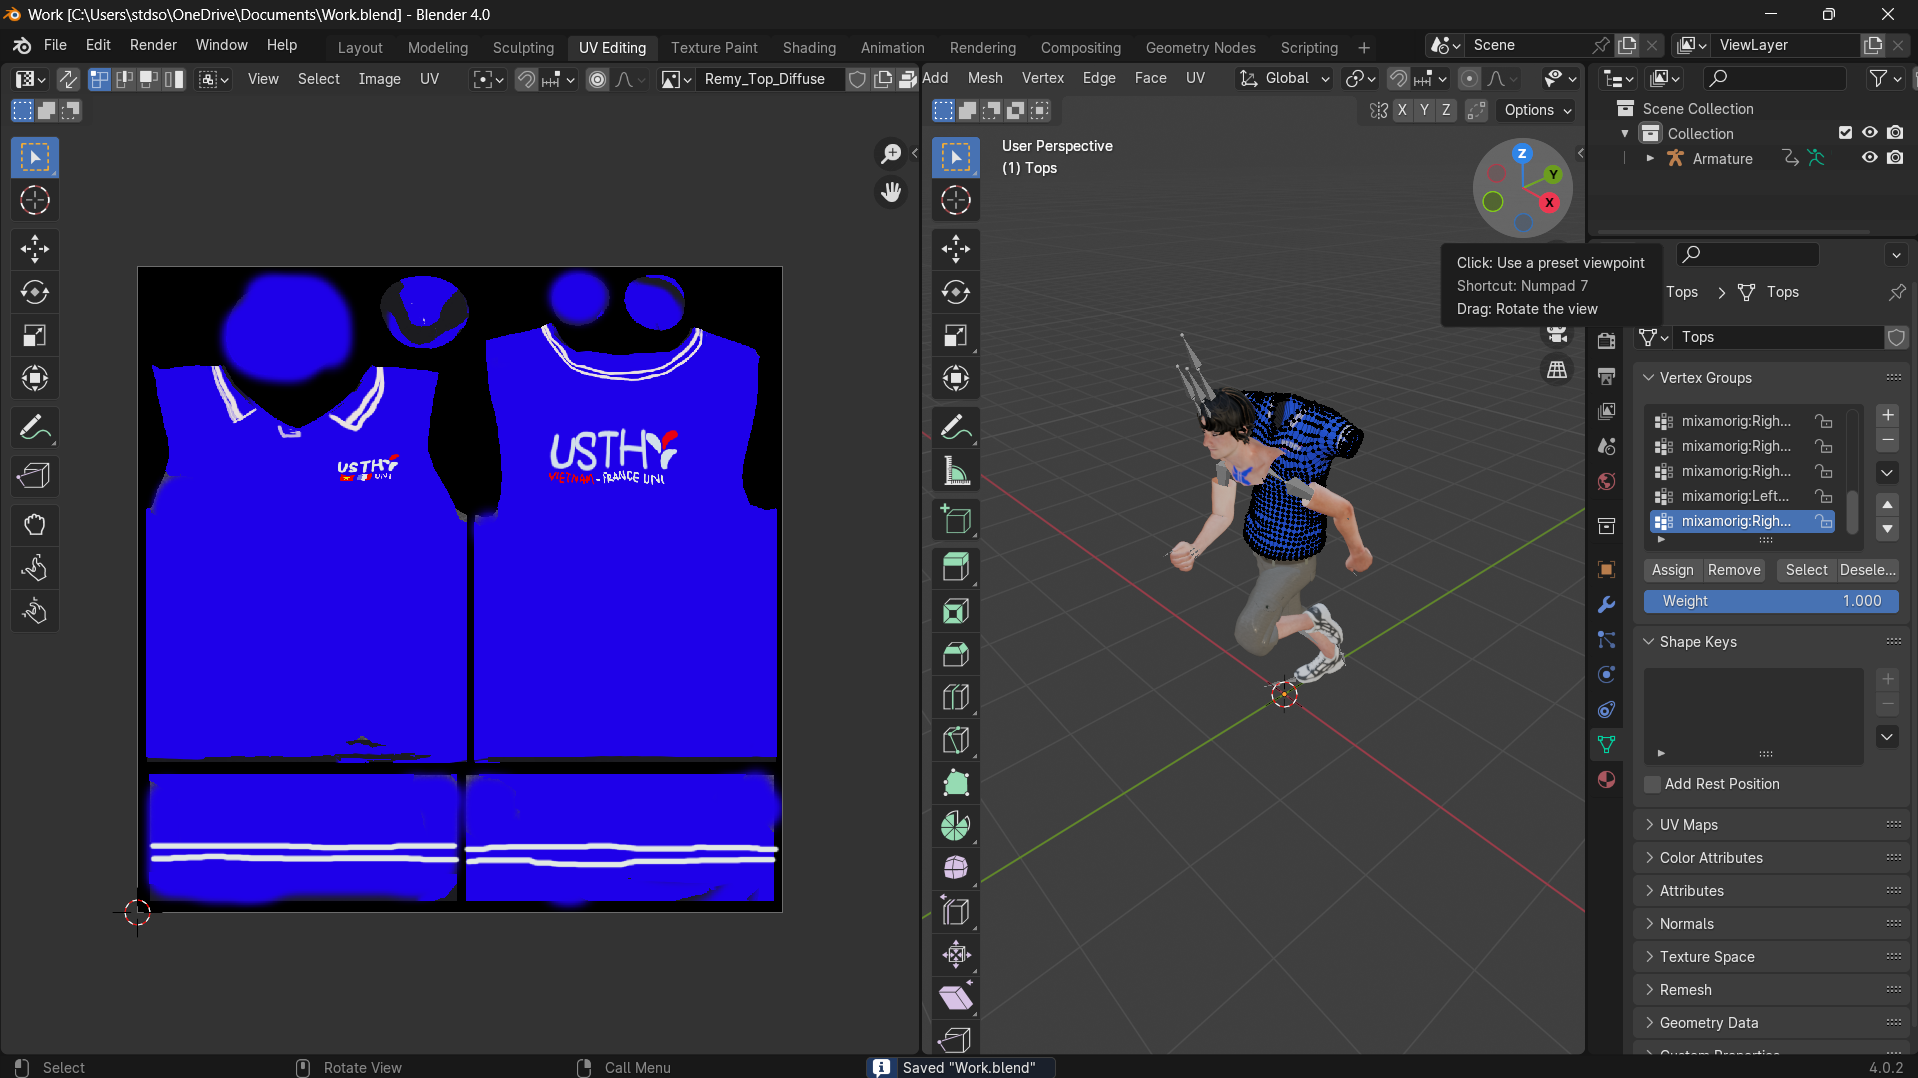
\includegraphics[width=0.49\textwidth]{market-blender.png}
    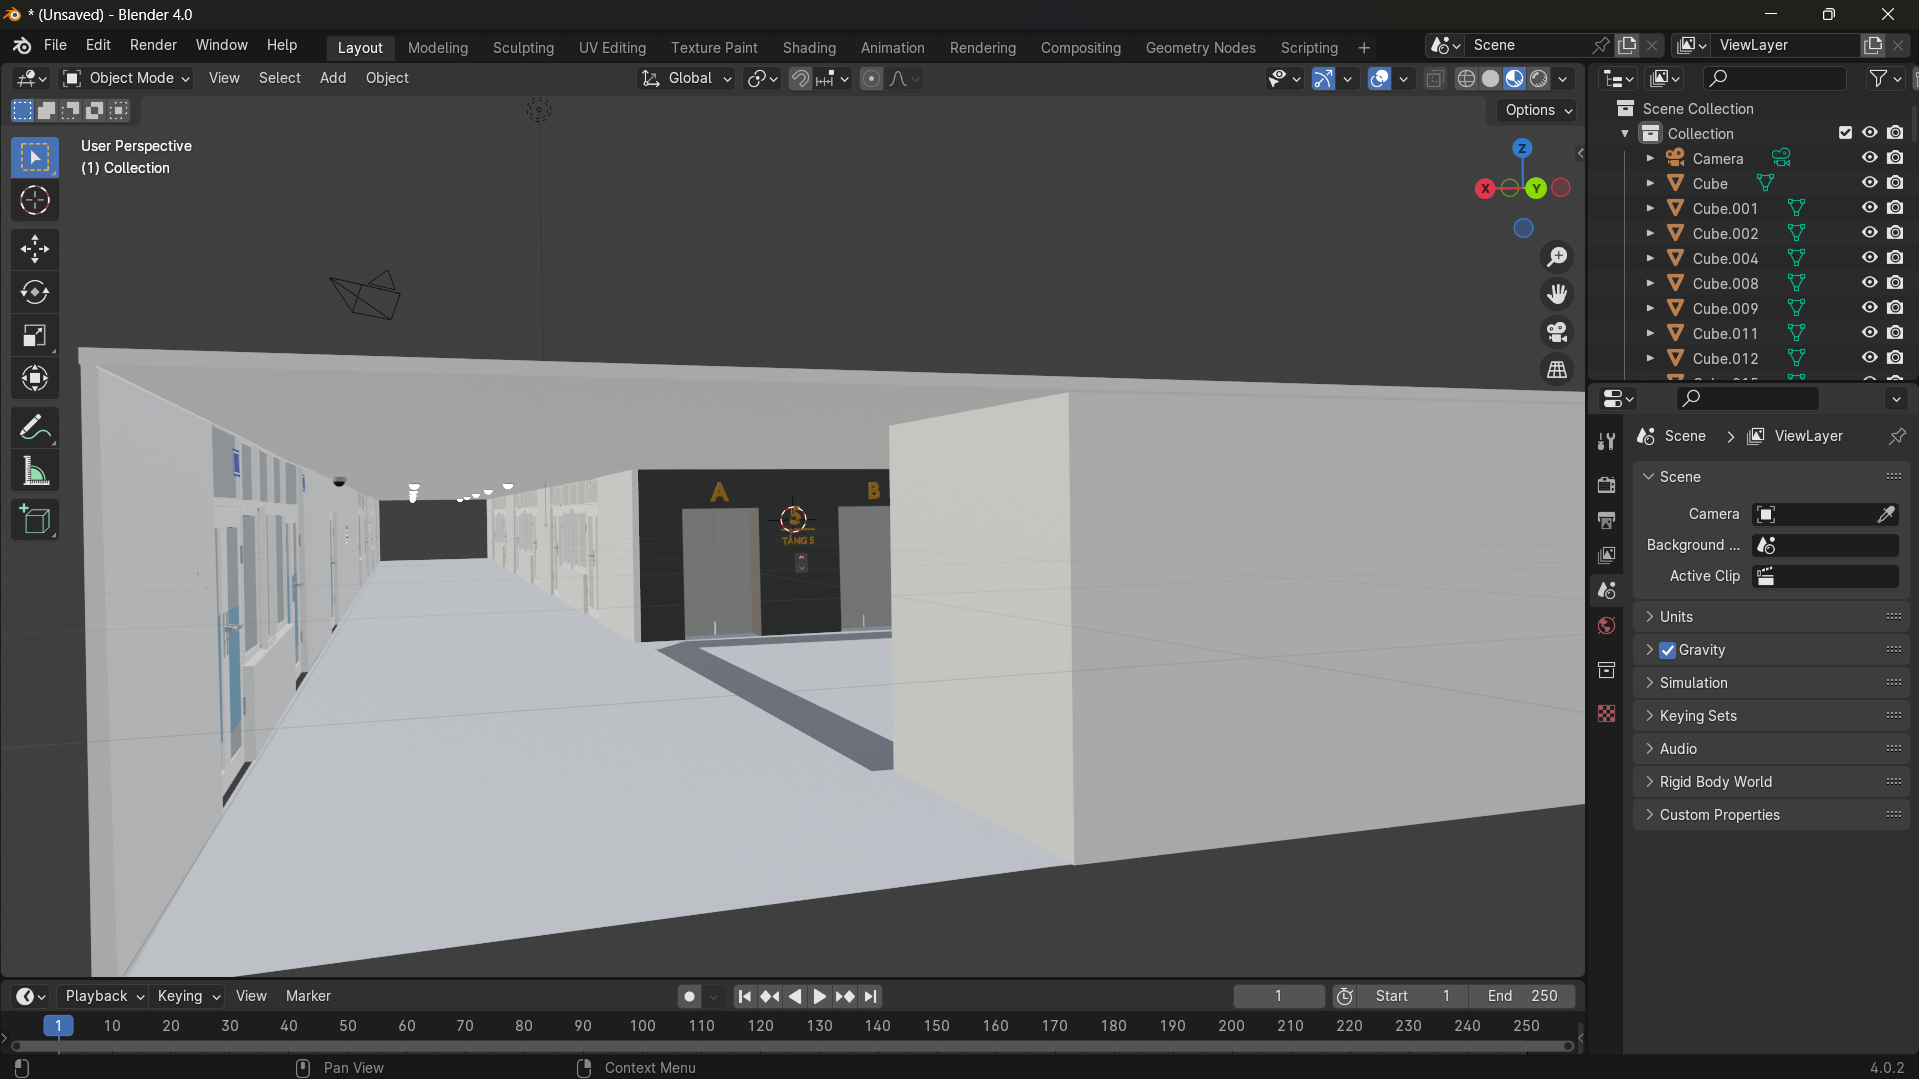
\includegraphics[width=0.49\textwidth]{blend.png}
    \caption{Blender Screenshots.}
\end{figure}
\subsubsection{Game Engine}
After testing multiple popular game engines, Unity emerged as the top choice for this project's game building application. Godot, although promising, still lacks the necessary features to properly build this project. On the other hand, Unreal Engine 5 from Epic Games is well-suited for the game due to its clear Python implementation support. However, its steep learning curve makes it less suitable for beginners to learn and build a game within a short timeframe.
\begin{figure}[ht]
    \centering
    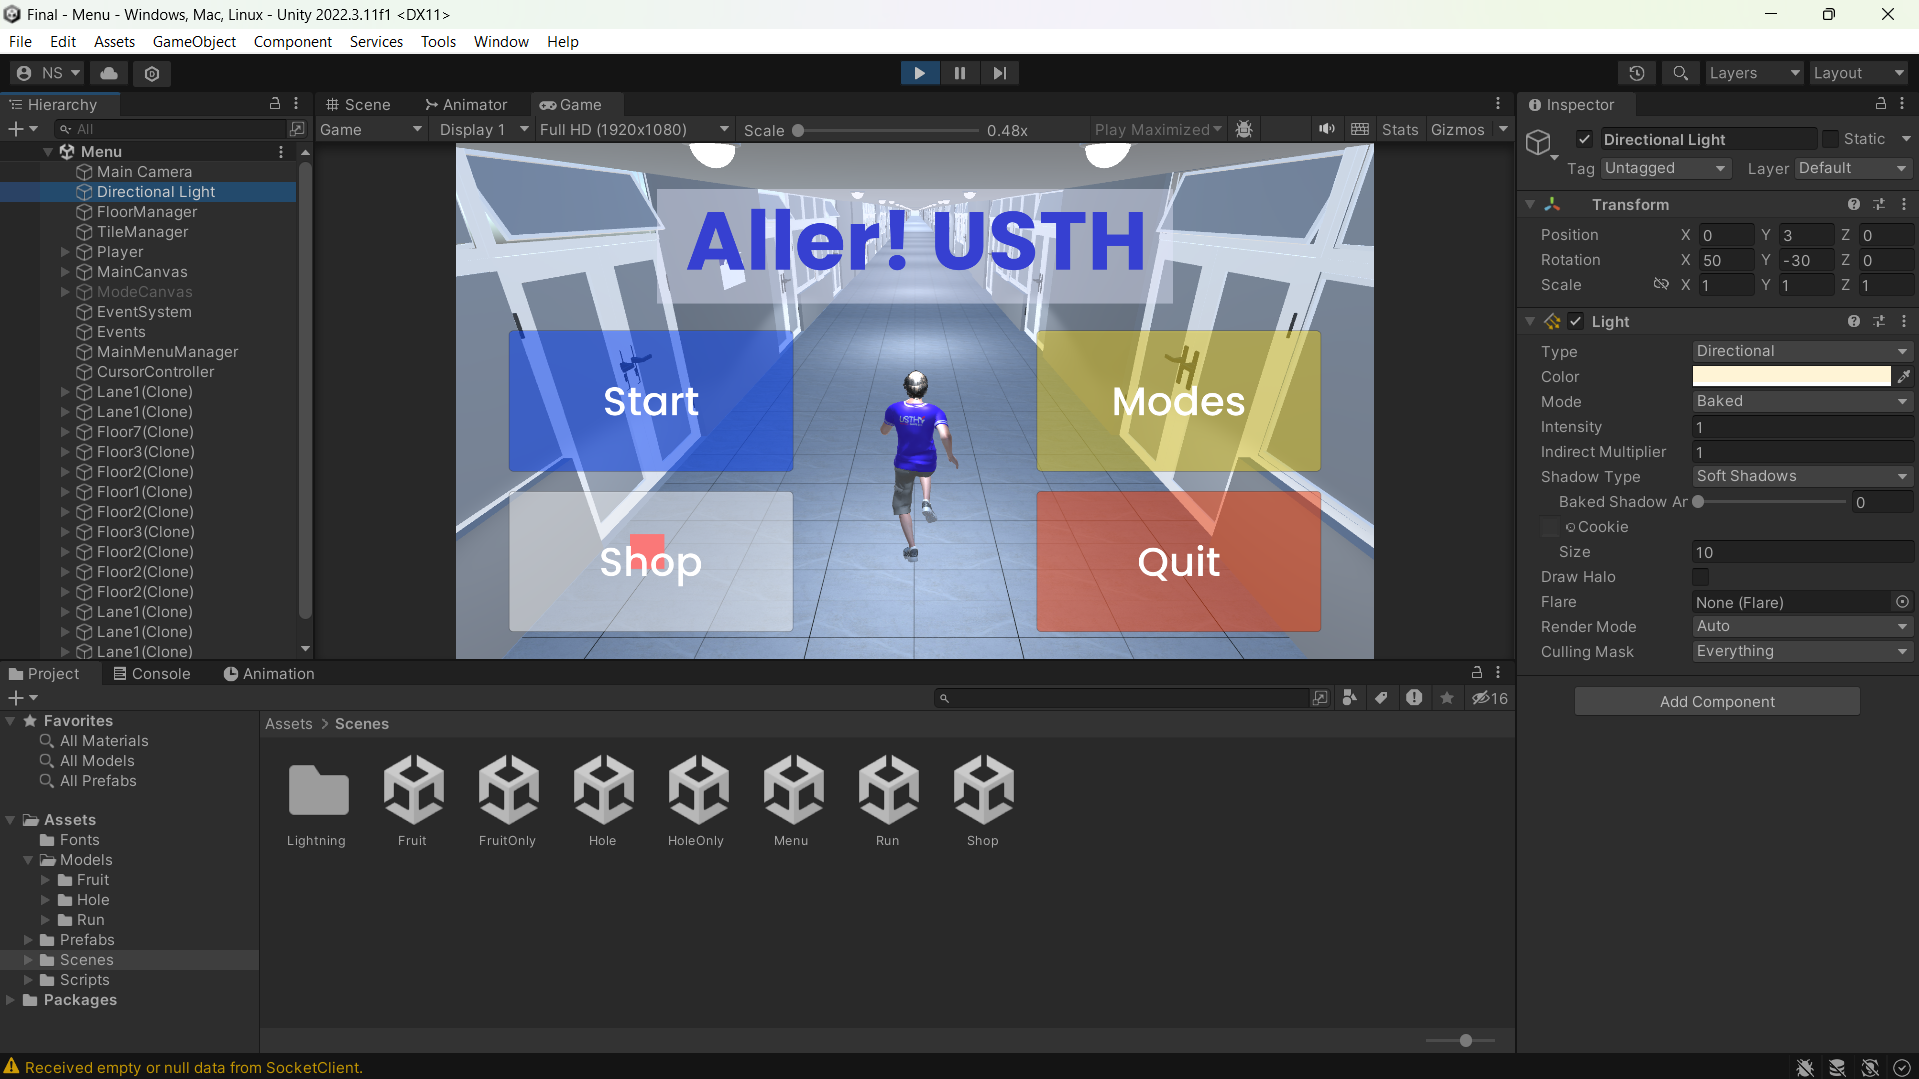
\includegraphics[width=0.75\textwidth]{unity.png}
    \caption{Unity Screenshot.}
\end{figure}
\clearpage

\section{MODEL}
\hspace*{1.5em}The landmark-tracking model is a critical component of Aller! USTH, and MediaPipe Pose and MoveNet were chosen for their accuracy, low latency, and widespread recognition within the developer community.\\

\begin{figure}[ht]
    \centering
    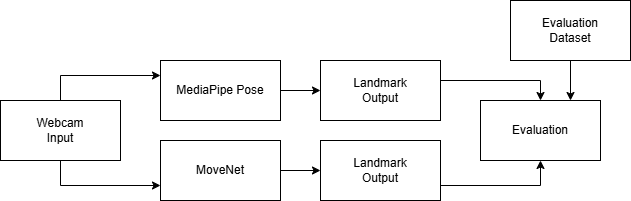
\includegraphics[width=0.9\textwidth]{ModelEva.drawio.png}
    \caption{Model Pipeline.}
\end{figure}

\subsection{Model Architecture}

\subsubsection{MediaPipe Pose}
\hspace*{1.5em}\textbf{Overview}\\[5pt]
MediaPipe Pose, developed by Google, is a real-time pose estimation solution capable of tracking key points of the human body. It's part of the MediaPipe framework, which supports various multimodal (audio, video, text) applied machine learning pipelines \cite{google2023}.  \\

\textbf{Keypoints}\\[5pt]
\hspace*{1.5em}- \textbf{Real-time Performance:} Can track human body key points in real time, making it ideal for interactive applications.\\[1pt]
\hspace*{1.5em}- \textbf{High Accuracy:} Provides precise detection of key body landmarks even in challenging conditions like occlusions and diverse poses.\\[1pt]
\hspace*{1.5em}- \textbf{Comprehensive Landmark Detection:} Detects 33 body landmarks, offering detailed pose estimation for applications requiring high precision.\\[1pt]

\subsubsection{MoveNet}
\hspace*{1.5em}\textbf{Overview:}\\[5pt]
MoveNet Lightning is a fast and precise pose estimation model designed for real-time applications. It is part of the MoveNet family, known for balancing speed and accuracy effectively. \cite{kaggle2024}.\\

\textbf{Keypoints}\\[5pt]
\hspace*{1.5em}- \textbf{Speed and Precision:} Optimized for high-speed detection without sacrificing much accuracy, making it suitable for dynamic activities like sports and fitness apps.\\[1pt]
\hspace*{1.5em}- \textbf{Lightweight Architecture:} Ensures smooth operation on both high-end and low-end devices, providing flexibility in deployment.\\[1pt]
\hspace*{1.5em}- \textbf{Simplified Landmark Detection:} Detects 17 key body landmarks, focusing on essential points for quick and reliable pose estimation.\\[1pt]

\textbf{Conclusion}\\[5pt]
Both MediaPipe Pose and MoveNet offer excellent capabilities for pose estimation, each with their own unique strengths.
MediaPipe Pose is chosen for its detailed landmark detection and robustness across various conditions. On the other hand, MoveNet is selected for its lightning-fast performance and suitability for real-time applications.
So either model could be an excellent choice for "Aller! USTH".

\subsection{Evaluation Data}
\subsubsection{COCO-WholeBody Dataset}
\textbf{COCO-WholeBody} is an extension of MS COCO (Microsoft Common Objects in Context) dataset with whole-body annotations. It was created by Sheng Jin, Lumin Xu, Jin Xu, Can Wang, Wentao Liu, Chen Qian, Wanli Ouyang, and Ping Luo and contains a large collection of images and corresponding annotations of human poses. We use a part of the original dataset for evaluation purposes only \cite{jin2020arxiv}.\\

\textbf{Key features of the COCO-WholeBody Dataset:}\\[5pt]
\hspace*{1.5em}- \textbf{Dataset size:} The dataset comprises approximately 164,000 images (25GB), making it one of the largest publicly available datasets for human pose estimation. For evaluation, we focused on the COCO2017 validation subset, which contains 5,000 images (1GB).\\[5pt]
\hspace*{1.5em}- \textbf{Annotations:} There are 4 types of bounding boxes (person box, face box, left-hand box, and right-hand box) and 133 keypoints (17 for body, 6 for feet, 68 for face, and 42 for hands) annotations for each person in the image. Only the 17 keypoints for the body were used in the evaluation process \cite{jin2020arxiv}.\\[5pt]
\hspace*{1.5em}- \textbf{Diversity:} The dataset contains images depicting people of different ages, genders, and body types, ensuring a diverse representation of human poses. This feature affects our evaluation results greatly because we only consider images that have the full body ground truth keypoints visible (all 17 keypoints), which decreases our data size to only 82 images to evaluate the models \cite{jin2020arxiv}.\\[5pt]
\hspace*{1.5em}- \textbf{Usage:} The data was used for evaluation purposes, more specifically to evaluate the percentage of correct keypoints (PCK) and the accuracy of the models.\\

\begin{figure}[ht]
    \centering
    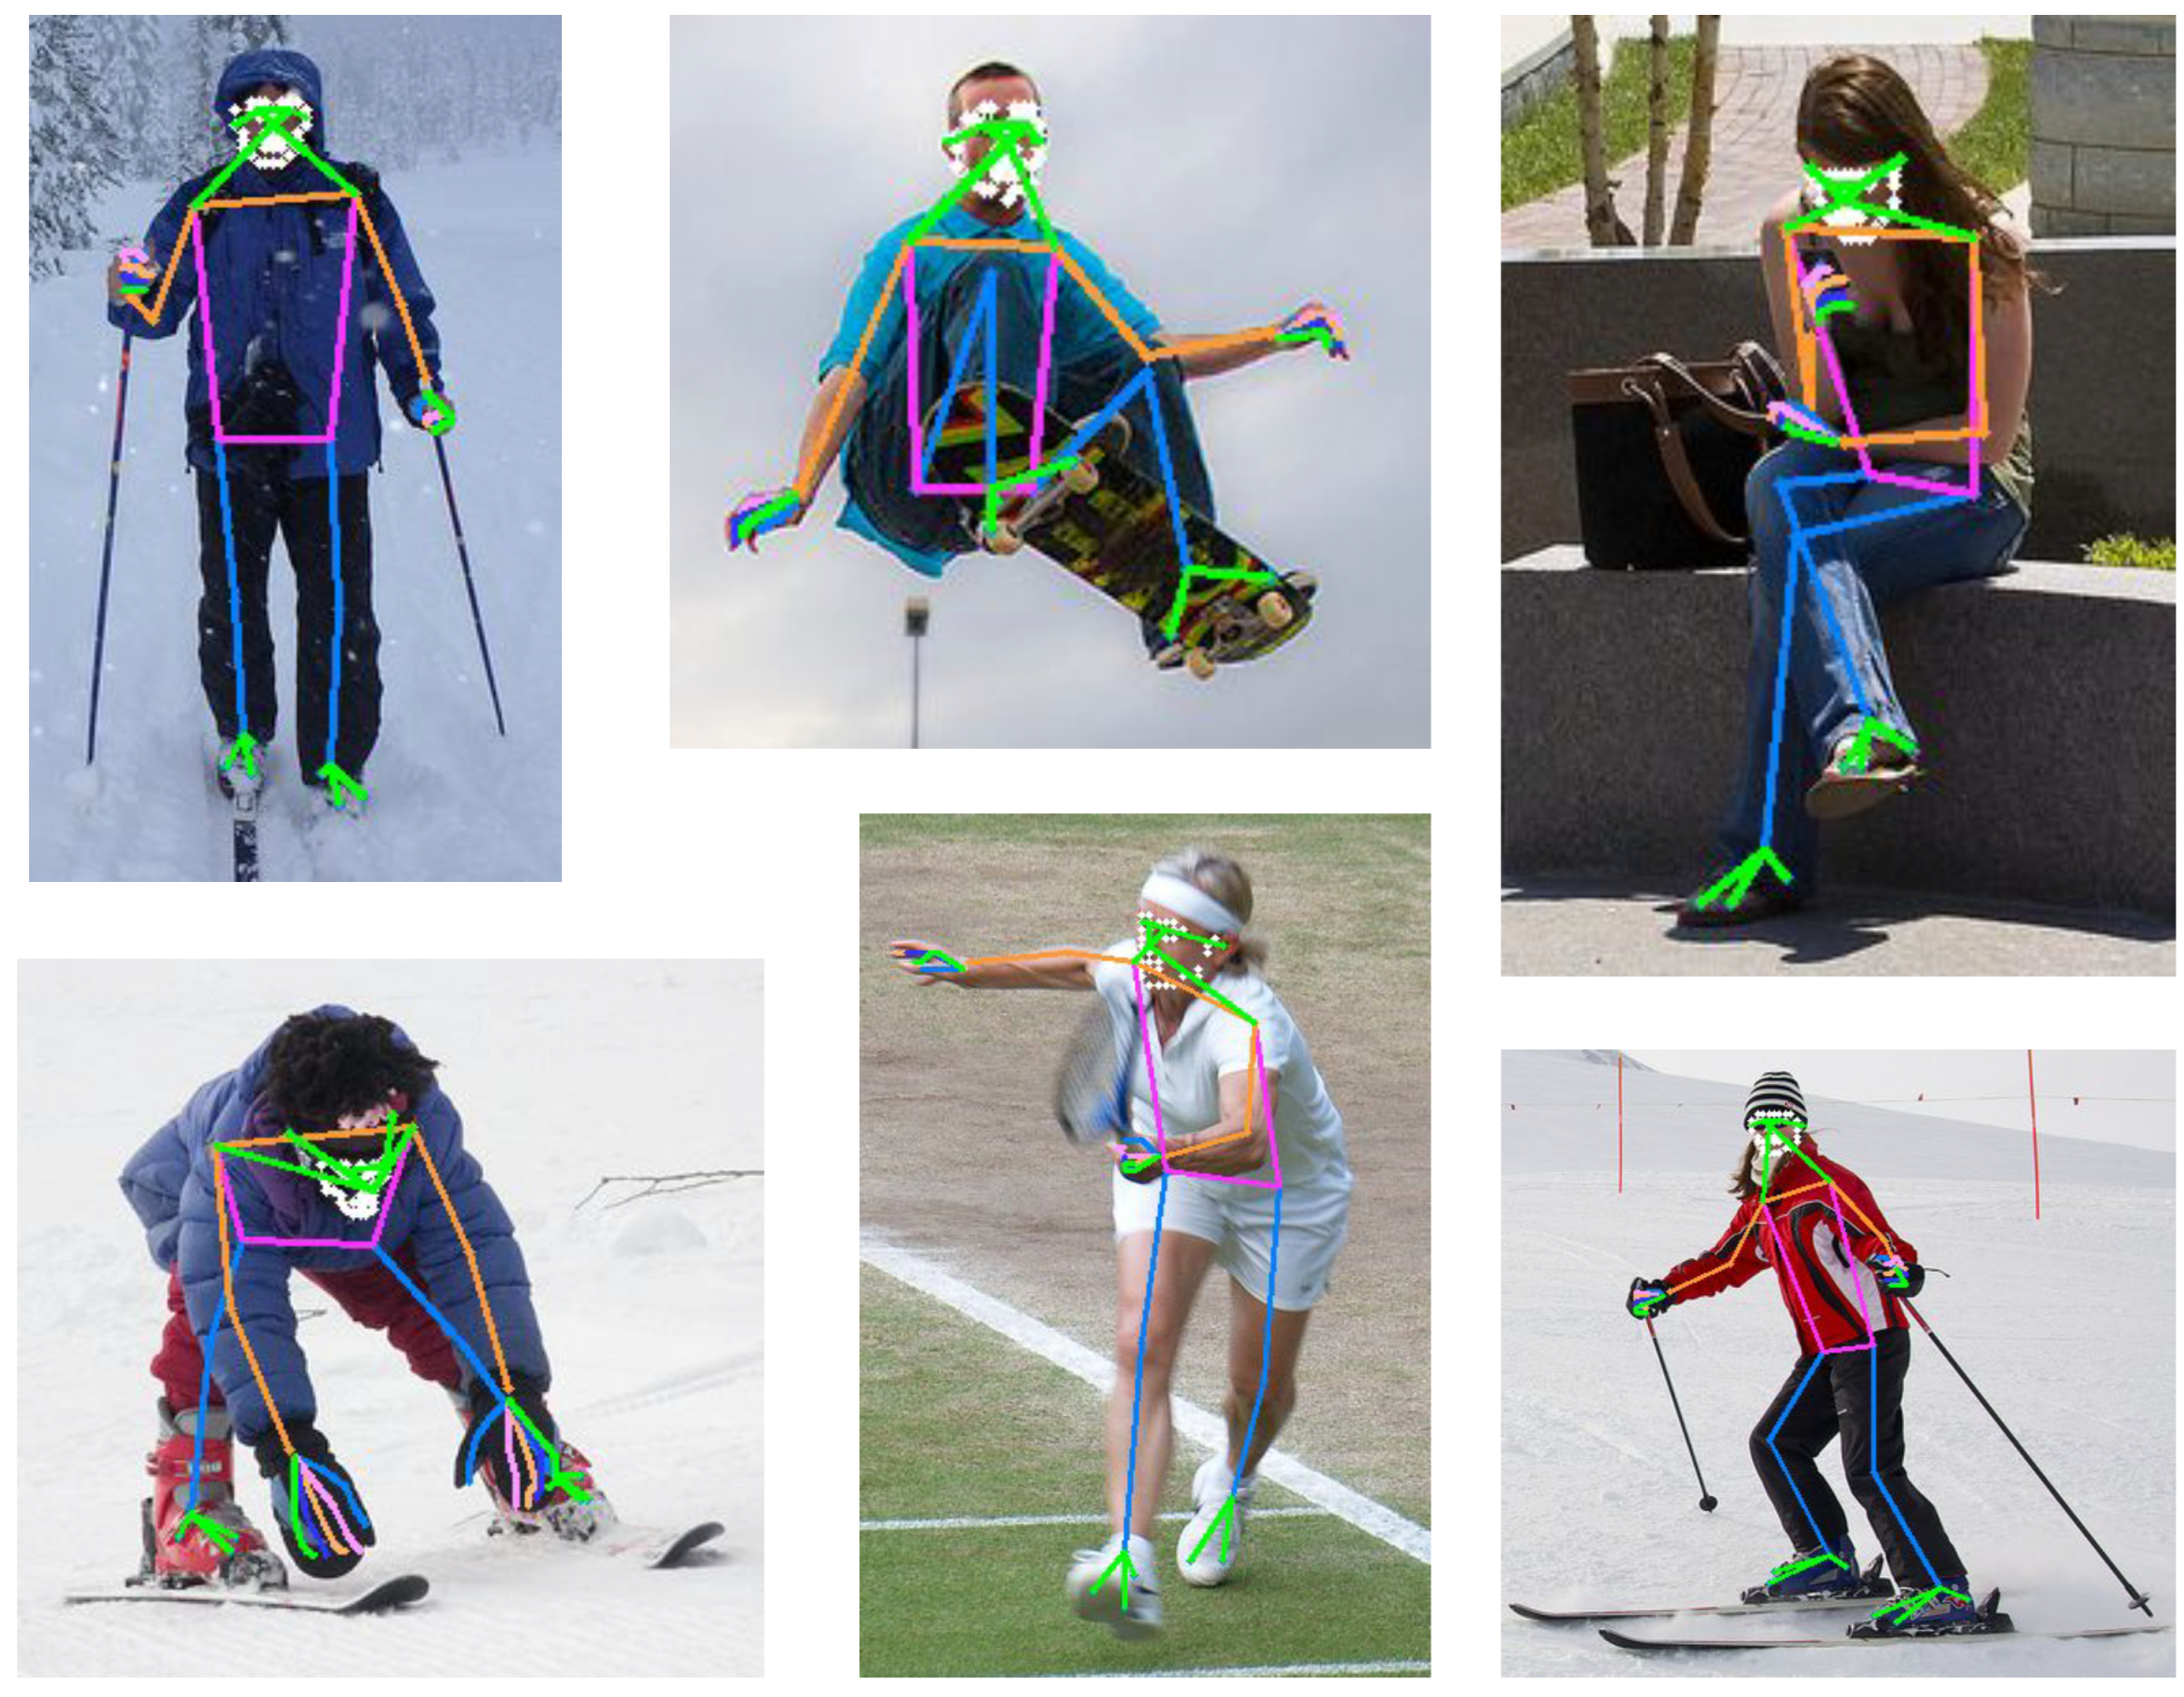
\includegraphics[width=0.7\textwidth]{coco.jpg}
    \caption{COCO-WholeBody Dataset for Evaluation.}
\end{figure}

\textbf{COCO-WholeBody Dataset Processing}\\[5pt]
\hspace*{1.5em}- \textbf{Download the Dataset:} The dataset can be downloaded from the GitHub link \cite{jin2020github}.\\[5pt]
\hspace*{1.5em}- \textbf{Annotation File Formats:} This dataset comes with annotation files in JSON formats. These annotation files contain information about the 2D joint positions for each image in detail about the coordinates of body joints in the dataset.\\[5pt]
\hspace*{1.5em}- \textbf{Data Augmentation:} The next step involves loading and parsing the annotation files. This process extracts the 2D joint positions for each image, which serve as ground truth data for model training and evaluation.\\[5pt]
\hspace*{1.5em}- \textbf{Filter out Unnecessary Data:} For this scenario, we accounted for the images with full body ground truth keypoints visible (all 17 keypoints) to make the comparison consistent across all keypoints and all models. We deemed images having 17 "num\_keypoints" annotation feature as valid and used another filter after that, taking every image with 17 "num\_keypoints" but also having multiple people in it (which means 1 image having multiple repetitive "image\_id" annotation feature) as invalid and will be removed. Result in a dataset with 82 images only.

\subsubsection{Friends' Landmarks Data}
\textbf{Friends' Landmarks Data} is a dataset created by me with the help of my friends and mates, a total of 18 people. It consists of video recordings and corresponding frame annotations focused on human poses during various simple activities. We use a part of the original dataset for evaluation purposes only.\\

\textbf{Key features of the Friends' Landmarks Data:}\\[5pt]
\hspace*{1.5em}- \textbf{Dataset size:} The dataset consists of 131 video recordings, with over 51,000 frames initially, totaling 1.53GB. After scanning and filtering, approximately 43,300 frames were deemed usable. Due to time limitations, 800 different frames were selected for this evaluation.\\[5pt]
\hspace*{1.5em}- \textbf{Types of activities:} The dataset includes simple movements like moving left or right one space, jumping in place, and crouching in place (for Subway Surfers); and hand activities such as waving while standing still (for Fruit Ninja and Hole in the Wall type games).\\[5pt]
\hspace*{1.5em}- \textbf{Annotations:} The dataset includes keypoint annotations with 13 different landmarks of the body: "nose", "left\_hand", "left\_elbow", "left\_shoulder", "right\_shoulder", "right\_elbow", "right\_hand", "left\_hip", "right\_hip", "left\_knee", "left\_foot", "right\_knee", "right\_foot". All 2,500 images are annotated for evaluation purposes.\\[5pt]
\hspace*{1.5em}- \textbf{Diversity:} The dataset contains images of people of different ages, genders, and body types. Most participants are aged 20-21, with two younger participants (ages 7 and 11). The group includes one girl aged 11, one female friend, and the rest are boys. The body types vary, with participants having a BMI ranging from under 15 to over 30. While the human body structure is similar, this diversity ensures a wide representation of human poses.\\[5pt]
\hspace*{1.5em}- \textbf{Usage:} The data was used for evaluation purposes, more specifically to evaluate the percentage of correct keypoints (PCK) and the accuracy of the models.\\

\textbf{Friends' Landmarks Data Processing}\\[5pt]
\hspace*{1.5em}- \textbf{Extract the frames: }The raw data includes videos in MP4 format. Then the video were extracted to be hundreds of frames in JPG format.\\[5pt]
\hspace*{1.5em}- \textbf{Annotate the landmarks: }The raw frames then got landmarks annotated using OpenCV like in the Figure below. 
The processed images are in JPG format, with keypoint annotations stored in TXT files.\\[5pt]
\begin{figure}[ht]
    \centering
    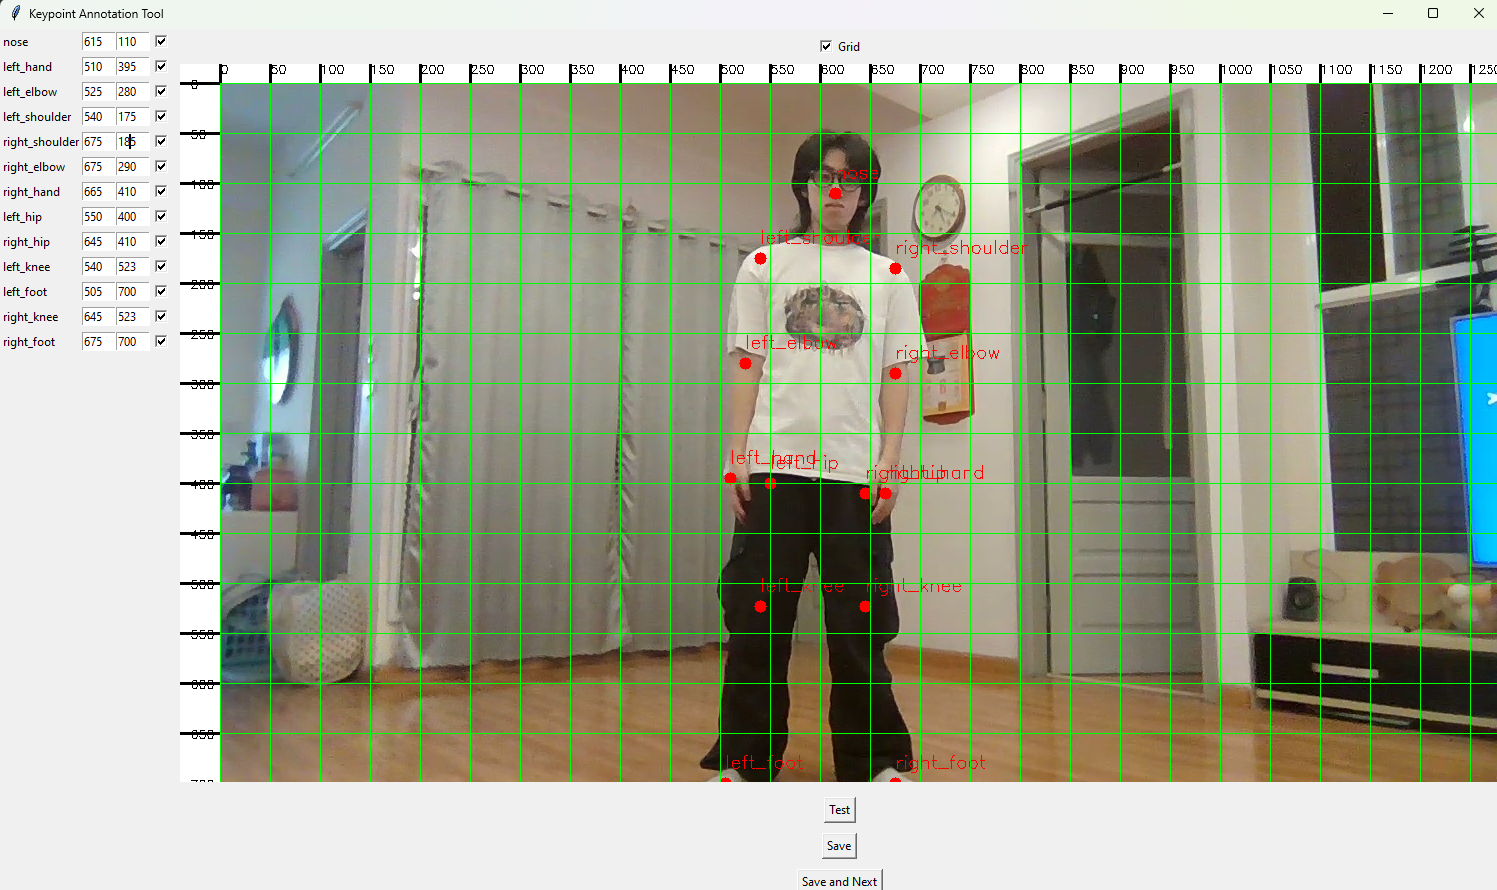
\includegraphics[width=1\textwidth]{friend1.png}
    \caption{Friends' Landmarks Data Annotating Process.}
\end{figure}

\begin{figure}[ht]
    \centering
    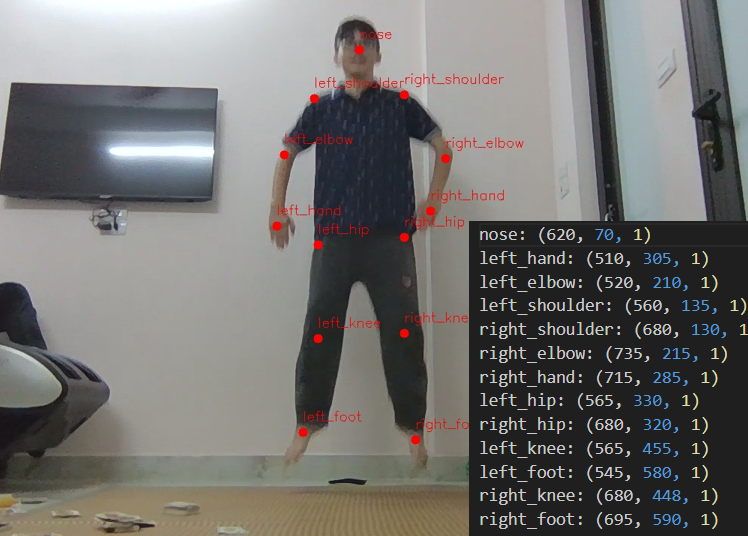
\includegraphics[width=0.45\textwidth]{friend3.png}
    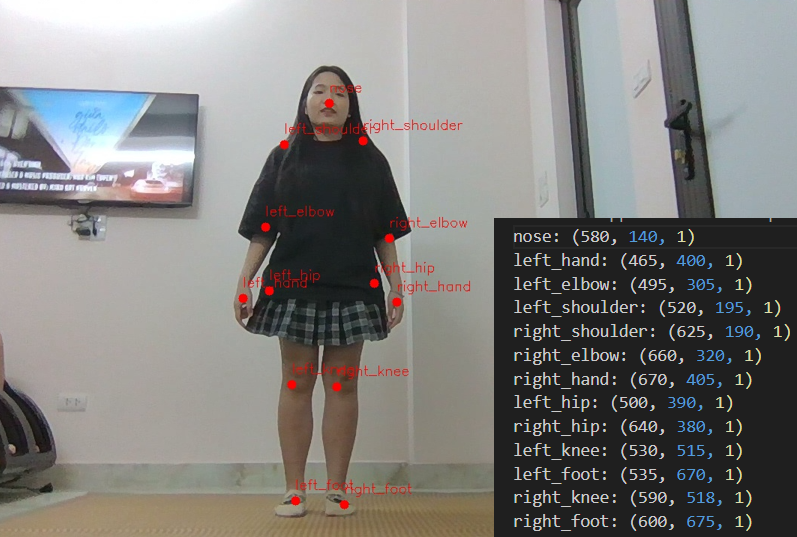
\includegraphics[width=0.5\textwidth]{friend4.png}
    \caption{Friends' Landmarks Dataset for Evaluation.}
\end{figure}

\clearpage
\subsection{Evaluation}

\subsubsection{Percentage of Correct Keypoints (PCK)}

\hspace*{1.5em}\textbf{Objective:} PCK is to evaluate the accuracy of predicted keypoints compared to the ground truth keypoints, how well can the model perform in different environments, and the distance of the person to the device’s webcam.\\

\textbf{Methodology:} To calculate how many correctly predicted keypoints over all keypoints. The detected keypoint is considered correct when the distance between the predicted location and the ground truth location is within a certain threshold. For this case, if the distance is lower than 0.05 of the torso distance, it is considered correct and wrong otherwise \cite{chung2022}.\\

\textbf{Distance between predicted keypoints and ground truth keypoints:}
\[
    d = \sqrt{(x_1 - x_2)^2 + (y_1 - y_2)^2}
\]
- \(x_1, y_1\): x,y coordinate of a ground truth keypoint\\
- \(x_2, y_2\): x,y coordinate of a predicted keypoint\\

\textbf{Diameter of the torso:}
\[
    d_{ts} = \sqrt{(x_{ls} - x_{rh})^2 + (y_{ls} - y_{rh})^2}
\]
- \(x_{ls}, y_{ls}\): x,y coordinate of the left shoulder keypoint\\
- \(x_{rh}, y_{rh}\): x,y coordinate of the right hip keypoint\\

\textbf{Percentage of Correct Keypoints:}
\[
    \frac{\sum_{i=1}^{n} \mathrm{bool}(d_i < 0.05 \cdot d_{ts})}{n}
\]
- If True: \(\text{bool}(d_i < 0.05 \cdot d_{ts}) = 1\)\\
- If False: \(\text{bool}(d_i < 0.05 \cdot d_{ts}) = 0\)\\
- \(n\): number of ground truth keypoints
\begin{figure}[ht]
    \centering
    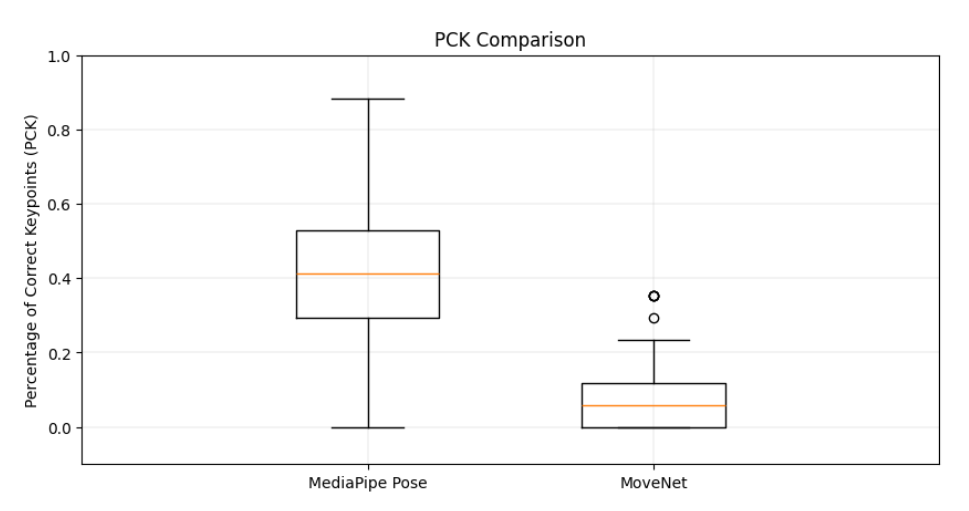
\includegraphics[width=0.8\textwidth]{pck.png}
    \caption{PCK Comparison between MediaPipe Pose and MoveNet.}
\end{figure}
\begin{table}[h]
    \centering
    \caption{Number of Images Recognized by Each Model for Specific PCK Ranges.}
    \begin{adjustbox}{width=\textwidth}
    \begin{tabular}{|c|c|c|c|c|c|}
        \hline
        & \textbf{PCK = 0} & \textbf{0$<$PCK$\le$0.25} & \textbf{0.25$<$PCK$\le$0.5} & \textbf{0.5$<$PCK$\le$0.75} & \textbf{0.75$<$PCK$\le$1} \\
        \hline
        \textbf{MediaPipe Pose} & 55 & 55 & 490 & 179 & 38 \\
        \hline
        \textbf{MoveNet} & 306 & 408 & 46 & 0 & 0 \\
        \hline
    \end{tabular}
    \end{adjustbox}
\end{table}
    
\textbf{Observation:} MediaPipe Pose achieved decent performance because it had the highest number of images in the third and fourth groups (25–75\%), indicating that 25\% to 75\% of the detected keypoints from 803 images were correctly matched with the ground truth. In contrast, MoveNet was found to have the poorest performance because it only had images in the first to third groups (0–50\%). In a total of 817 images, less than 50\% of the detected keypoints were correctly matched with the ground truth.


\subsubsection{Accuracy}

\hspace*{1.5em}\textbf{Objective:} We came up with this evaluation method based on PCK@0.2 to further understand the performance of both models, specifically on how accurately each keypoint was detected.\\

\textbf{Methodology:} To calculate how accurate the detected keypoint is compared to the ground truth keypoint. We take 1 minus the distance between the predicted location and the ground truth location over 0.2 of the torso distance. The result is the percentage of accuracy. If it is negative, we consider it to be 0\%. After that, we calculate the mean of every keypoint across the whole dataset \cite{chung2022}.\\

\textbf{Accuracy of every predicted keypoint given 0.2 of torso diameter as denominator:}
\[
    \displaystyle
    acc = 1 - \frac{d}{0.2 \cdot d_{ts}}
    \quad
    \displaystyle
    acc = \begin{cases}
        acc & \text{if } acc > 0    \\
        0   & \text{if } acc \leq 0
    \end{cases}
\]
- \(d\): Distance between predicted keypoints and ground truth keypoints\\
- \(d_{ts}\): Diameter of the torso\\

\textbf{Mean of every keypoint across the whole dataset:}
\[
    \displaystyle
    \text{mean\_acc}_i = \frac{\sum_{j=1}^{n} acc_{i,j}}{n}
\]
- \(i\): keypoint index\\
- \(j\): image index\\
- \(n\): number of images in the dataset\\

\begin{figure}[ht]
    \centering
    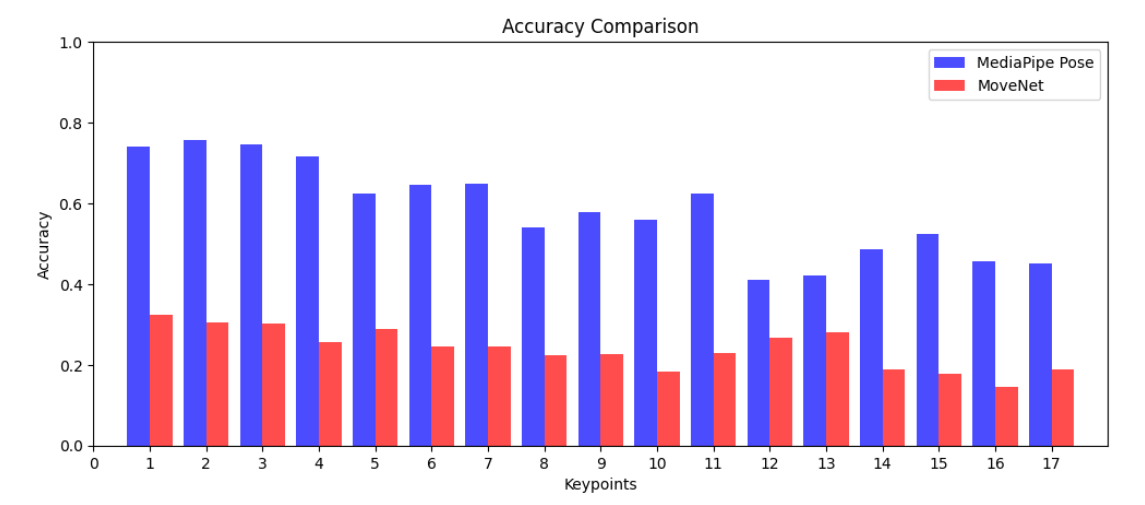
\includegraphics[width=1\textwidth]{accucom.png}
    \caption{Keypoint Detection Accuracy Comparison between MediaPipe Pose and MoveNet.}
\end{figure}

\textbf{Observation:} MediaPipe Pose consistently shows higher accuracy across nearly all keypoints compared to MoveNet (45\% to 75\% accuracy for MediaPipe compared to 14\% to 32\% accuracy for MoveNet). This indicates that MoveNet has difficulty predicting keypoints on diverse datasets (since it is recommended to use MoveNet on a single person who is 3ft ~ 6ft away from the device’s webcam)

\subsubsection{Precision}

\hspace*{1.5em}\textbf{Objective:} Precision is to evaluate the consistency of the models on their predictions, observing the predicted keypoints for any noticeable fluctuation, whether they are decently stable or rapidly volatile on video and real-time data.\\

\textbf{Methodology:} To calculate how precise or consistent the predicted keypoint is. We take a video of a visibly almost stationary human torso (in this case 472 frames, 640x480 resolution), get an array of the locations of the center point (average of 4 keypoints: left/right shoulder and left/right hip), and calculate the standard deviation of the array \cite{chung2022}.\\

- \textbf{Predicted center point location based on the 4 keypoints of the observed torso:}
\[
    \text{center} = \frac{k_{ls} + k_{rs} + \frac{k_{lh} + k_{rh}}{2}}{3}
\]
- \(k_{ls}, k_{rs}, k_{lh}, k_{rh}\): keypoint location of left shoulder, right shoulder, left hip, right hip respectively.\\

- \textbf{Standard deviation of the x-axis:}
\[
    \text{std}_x = \sqrt{\frac{\sum_{i=1}^{n} (x_i - \bar{x})^2}{n}}
\]
- \(x_i\): x coordinate of a predicted center point at i frame\\
- \(\bar{x}\): mean of the x coordinate of predicted center points across all frames\\
- \(n\): number of frames in the input video\\

- \textbf{Standard deviation of the y-axis:}
\[
    \text{std}_y = \sqrt{\frac{\sum_{i=1}^{n} (y_i - \bar{y})^2}{n}}
\]
- \(y_i\): y coordinate of a predicted center point at i frame\\
- \(\bar{y}\): mean of y coordinate of predicted center points across all frames
\begin{table}[h]
    \centering
    \caption{Number of Images Recognized by Each Model for Specific PCK Ranges.}
    \begin{tabular}{|c|c|c|}
        \hline
        & \textbf{MediaPipe Pose} & \textbf{MoveNet}\\
        \hline
        \textbf{MediaPipe Pose} & 55 & 55  \\
        \hline
        \textbf{MoveNet} & 306 & 408  \\
        \hline
    \end{tabular}
\end{table}

\FloatBarrier

\begin{figure}[ht]
    \centering
    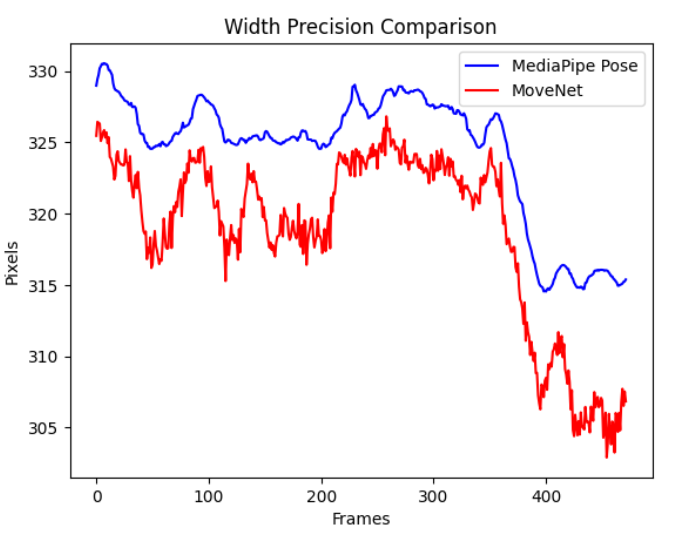
\includegraphics[width=0.5\textwidth]{prew.png}
    \caption{Width Precision Comparison between MediaPipe Pose and MoveNet.}
\end{figure}

\FloatBarrier

\begin{figure}[ht]
    \centering
    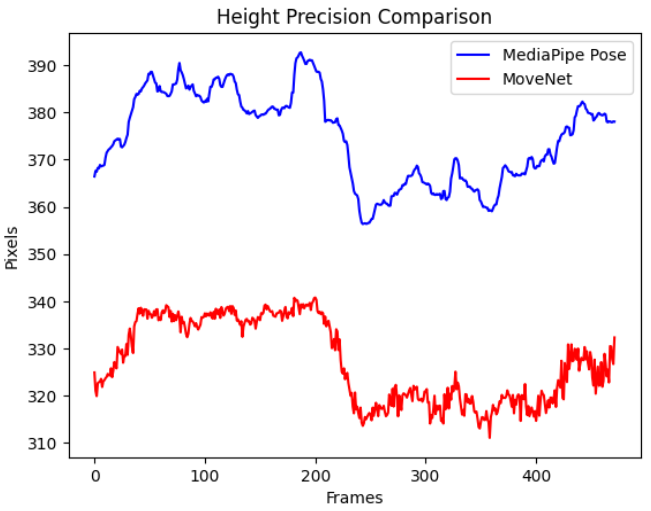
\includegraphics[width=0.5\textwidth]{preh.png}
    \caption{Height Precision Comparison between MediaPipe Pose and MoveNet.}
\end{figure}

\FloatBarrier

\textbf{Observation:} The chart shows fluctuations in the predicted pixels for both models, MediaPipe’s predictions seem to be more stable with less variation, whereas MoveNet shows more volatility but is still decently stable for our project. While MediaPipe can perform well in various situations such as close to mid-range from the user to their device’s webcam, MoveNet struggles in close-range scenarios, but this problem is very niche in our project. We can also observe MoveNet’s lack of accuracy from the 2 graphs above \cite{chung2022}.

\subsubsection{FPS and Processing Time/Delay}

\hspace*{1.5em}\textbf{Objective:} To estimate the frame per second (FPS) and evaluate how smoothly the model performs on real-time data and to calculate the delay between 2 frames, which is also the delay time between the user’s action and the game’s output action.\\

\textbf{Methodology:} To calculate how many frames the model can process in 1 second and the time needed to process between 2 frames, we need to take the overall frames of the input video data divided by the overall time needed to process the video to get the FPS, then take 1 divided by FPS to get the processing time between 2 frames.\\

- \textbf{FPS:}
\[
    \text{FPS} = \frac{\text{overall frames of a video}}{\text{overall processing time needed}}
\]

- \textbf{Processing time/delay:}
\[
    \text{Processing time/delay} = \frac{1}{\text{FPS}}
\]

\begin{table}[h]
    \centering
    \caption{FPS and Delay Comparison between MediaPipe Pose and MoveNet.}
    \begin{tabular}{|l|c|c|}
    \hline
     & \textbf{MediaPipe Pose} & \textbf{MoveNet} \\
     \hline
    \textbf{FPS} & 29 & 49 \\
    \hline
    \textbf{Delay} & 34.37153414144355 (ms) & 20.359124167490812 (ms) \\
    \hline    
    \end{tabular}
    \end{table}
    
    \subsubsection{Final Results}
    We conclude the pros/cons:
    
    \begin{table}[h]
    \centering
    \caption{Pros and Cons of MediaPipe Pose and MoveNet.}
    \begin{adjustbox}{width=\textwidth}
    \begin{tabular}{|l|p{0.45\textwidth}|p{0.45\textwidth}|}
    \hline
     & \textbf{MediaPipe Pose} & \textbf{MoveNet} \\
     \hline
    \textbf{Pros} & 
    - The models come with the package that can easily be installed and imported, there are API codes that already have built-in modules to predict, and draw keypoints, draw edges \newline
    → Beginner-friendly, very suitable for fast testing. \newline
    - The prediction range can go outside of the frame which makes the center point very consistent and accurate. & 
    - A fast and lightweight model ensuring minimum delay (faster than MediaPipe by 68.8\%) while having moderate accuracy and decent stability at mid-range. \newline
    → Less delay and better gaming experience (the most important factor for our project). \\
    \hline
    \textbf{Cons} & 
    - Faring slower than MoveNet (more time needed to process) results in more delay. \newline
    - Does not support transfer learning or fine-tuning. & 
    - Limited range of prediction [0,1] which makes the center point inconsistent when crouching because lower parts are bounded by the camera frame (only happens when standing too close to play). \newline
    - Does not support transfer learning or fine-tuning. \\
    \hline
    \end{tabular}
    \end{adjustbox}
    \end{table}
\clearpage

\section{GAME DESIGN}
\subsection{Model Implementation Design}

\begin{figure}[ht]
    \centering
    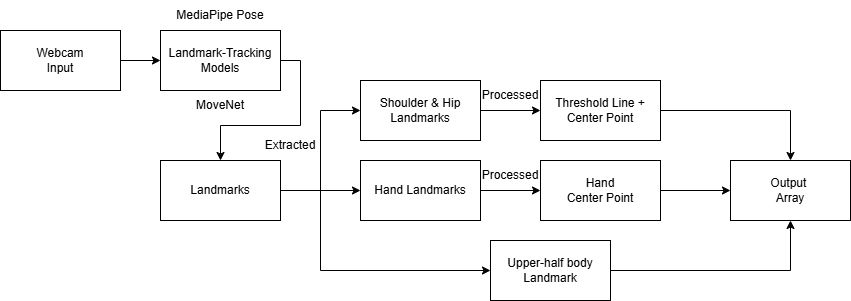
\includegraphics[width=1\textwidth]{ModelIm.drawio.png}
    \caption{Model Implementation Pipeline.}
\end{figure}

The process begins by initializing a video capture object using OpenCV. This library accesses the webcam, allowing us to capture live video frames. The captured frames are continuously fed into the system, providing real-time data for processing. \\

Next, the code sets up the landmark-tracking models from the models, specifically the Pose and Hands solutions. These models are initialized with confidence thresholds to ensure they provide accurate and reliable landmark detection. The Pose model is responsible for identifying key points on the body, such as the shoulders and hips. The Hands model focuses on detecting and tracking the hand landmarks, including key points like the wrists, thumbs, and fingertips.\\

Each frame captured from the webcam is converted from BGR to RGB since the MediaPipe models work with RGB images. The Pose model processes these RGB frames to identify and extract landmarks. These landmarks are the coordinates of key points on the body, which are then used for further calculations.
The same goes for the Hands model, which processes the frames to extract landmarks specific to the hands. This involves detecting the positions of the wrist, thumb, index finger, middle finger, ring finger, and pinky.\\

\begin{figure}[ht]
    \centering
    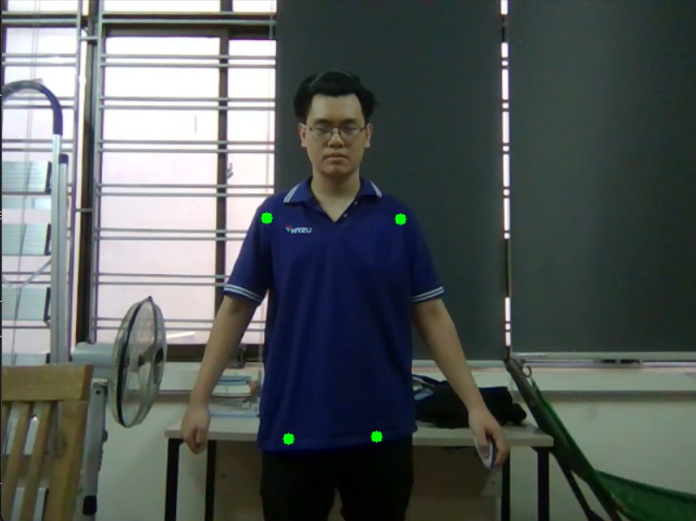
\includegraphics[width=0.4\textwidth]{pose1.png}
    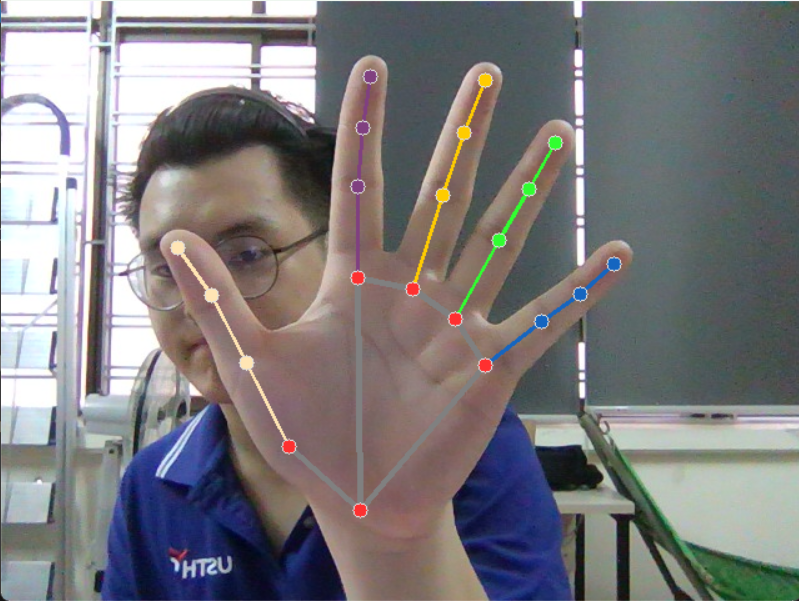
\includegraphics[width=0.4\textwidth]{hand3.png}
    \caption{Original Landmark Position (Left: Shoulder \& Hip; Right: Hand).}
\end{figure}

Once the landmarks are extracted, the code calculates the center points of both the body and the hands. For the body, it computes the average position of the shoulders and hips to find the body’s center. This center point helps in understanding the overall position and orientation of the user.\\

For the hands, the code calculates the center point by averaging the positions of the wrist, index finger, and pinky. This hand center point is crucial for gesture recognition and tracking hand movements accurately.\\

The shoulder and hip landmarks undergo additional processing to derive meaningful metrics. This includes calculating distances, angles, and relative positions. These processed landmarks are essential for understanding the user's posture and movements. For instance, by tracking the movement of the shoulders and hips, the system can determine if the user is standing, sitting, or moving in a specific direction.\\

\begin{figure}[ht]
    \centering
    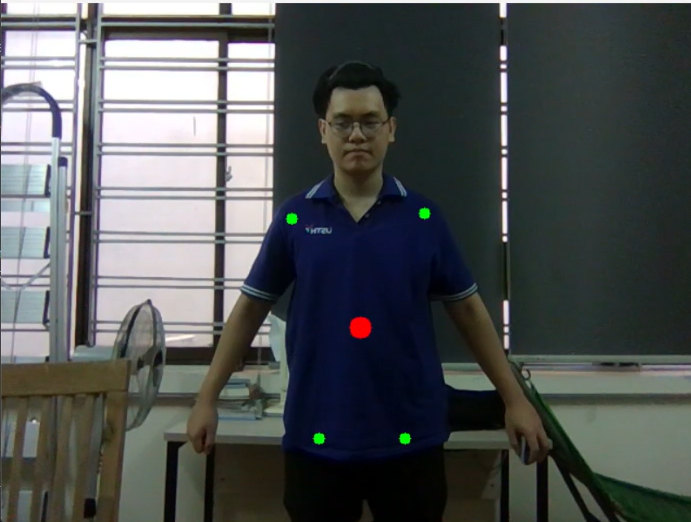
\includegraphics[width=0.4\textwidth]{pose2.png}
    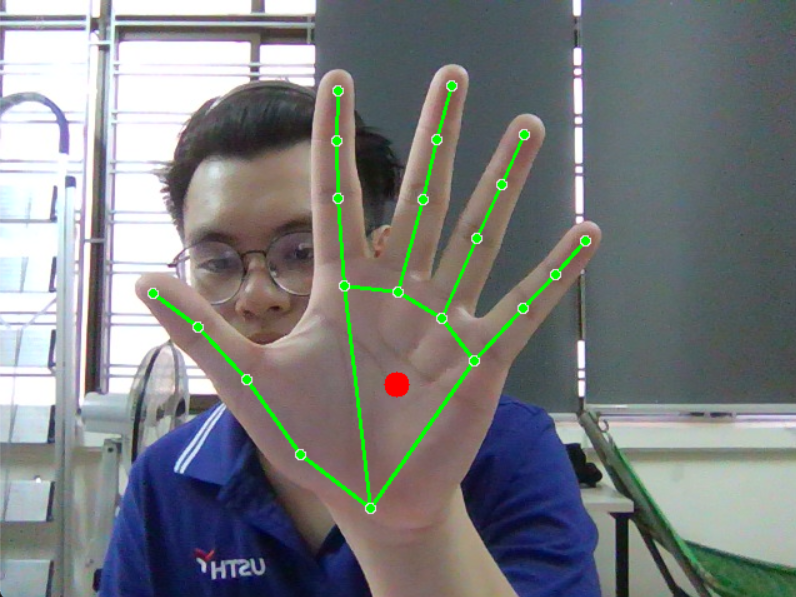
\includegraphics[width=0.4\textwidth]{hand2.png}
    \caption{Center Landmark (Left: Body; Right: Hand).}
\end{figure}

Threshold lines are established based on the processed shoulder and hip landmarks. These lines act as boundaries to detect significant movements such as clapping or moving left and right. By monitoring the position of the body’s center relative to these threshold lines, the system can detect when the user crosses these boundaries, triggering specific actions.\\

\begin{figure}[ht]
    \centering
    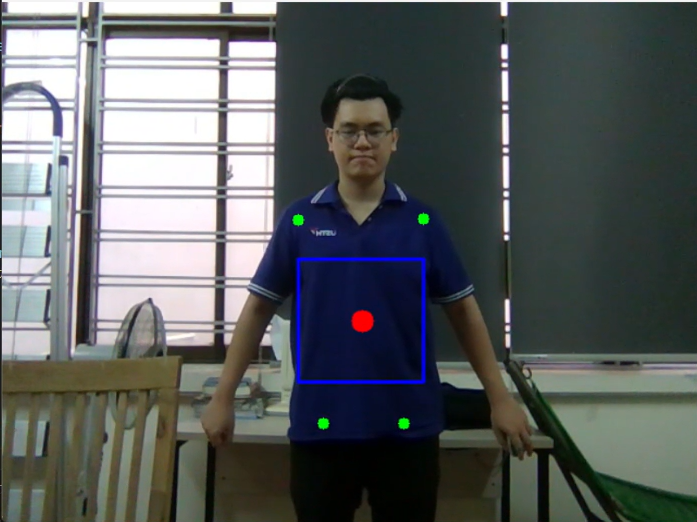
\includegraphics[width=0.4\textwidth]{pose3.png}
    \caption{Center Landmark with Threshold lines.}
\end{figure}

In addition to processing the shoulder and hip landmarks, the code also focuses on upper-half body landmarks. This includes tracking the positions of the nose and whole arms. These landmarks provide a more detailed understanding of the upper body’s movements.\\

\begin{figure}[ht]
    \centering
    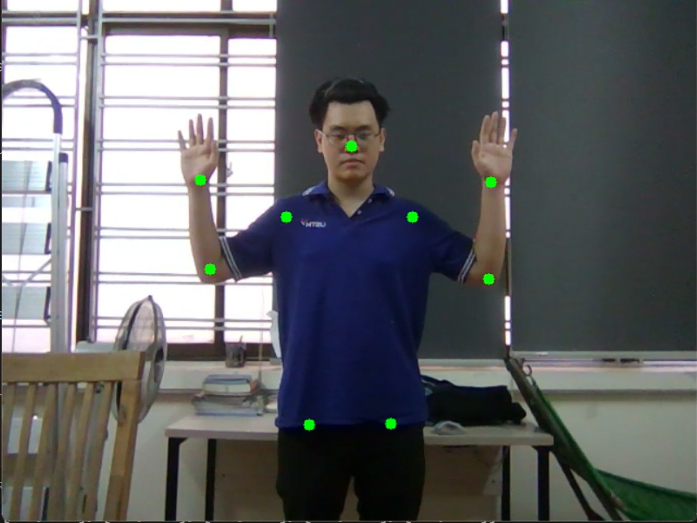
\includegraphics[width=0.4\textwidth]{pose4.png}
    \caption{Upper Body Landmark.}
\end{figure}

Finally, the results from all these calculations are combined into an output array. This array encapsulates the center points of the body and hands, the positions of various landmarks, and any detected movements or gestures. The output array is structured in a way that it can be easily interpreted and used by Socket later on.\\
\begin{figure}[ht]
    \centering
    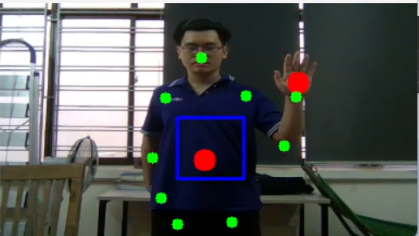
\includegraphics[width=0.4\textwidth]{all.png}
    \caption{All Body Landmarks Together.}
\end{figure}

\subsection{System Design and Analysis}
\subsubsection{System Requirement}
\hspace*{1.5em}\textbf{Minimum Requirement}\\[5pt]
-	GPU: Graphics card with OpenGL 3.0 or DirectX 9.0c support.\\
-	RAM: 4GB or higher.\\
-	Storage: 2GB of free disk space.\\
-	Display: 1280x720 resolution or higher.\\

\textbf{Recommended Requirement}\\[5pt]
-	GPU: Graphics card with support for OpenGL 4.x or DirectX 11.\\
-	RAM: 8GB or higher.\\
-	Storage: SD with at least 4GB of free disk space.\\
-	Display: 1920x1080 resolution or higher.

\subsubsection{Game Flow}
\begin{figure}[H]
    \centering
    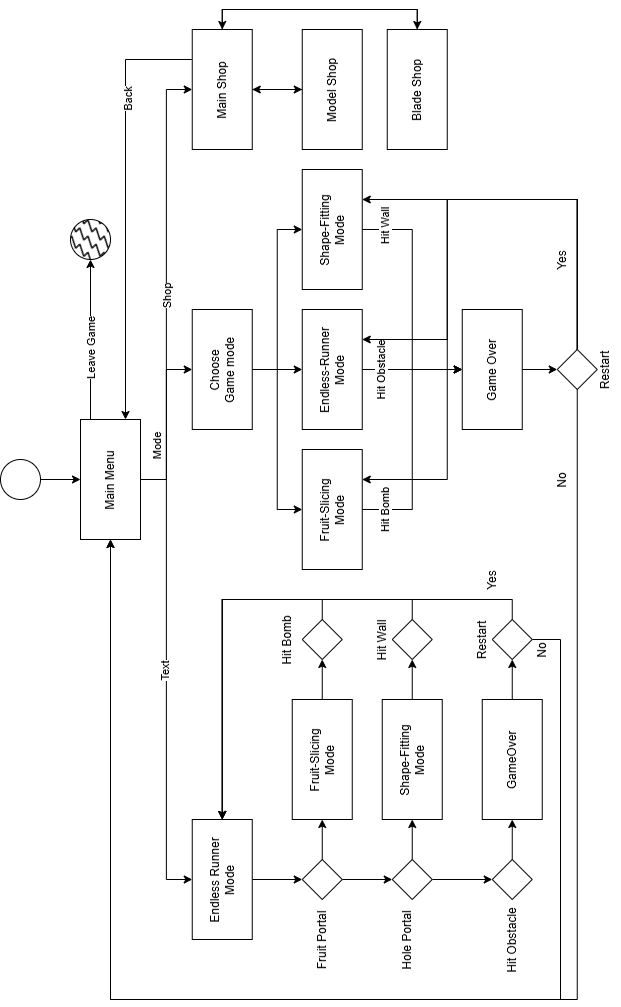
\includegraphics[width=0.8\textwidth]{flow4.drawio.png}
    \caption{Game Flow.}
\end{figure}
\clearpage

\subsection{Game Assets}
\hspace*{1.5em}There are so many assets in this game, from the Player model to the entire hallways with such small details like the door, the floor number... 
Unfortunately, because of the time constraint, not all of the assets of this game was originally created. 

\subsubsection{Player Model}
\hspace*{1.5em}After many attempts to create a Player model and rig it in order to put in the animation, it took about 3 weeks to create this model and fully animate it.\\
\begin{figure}[H]
    \centering
    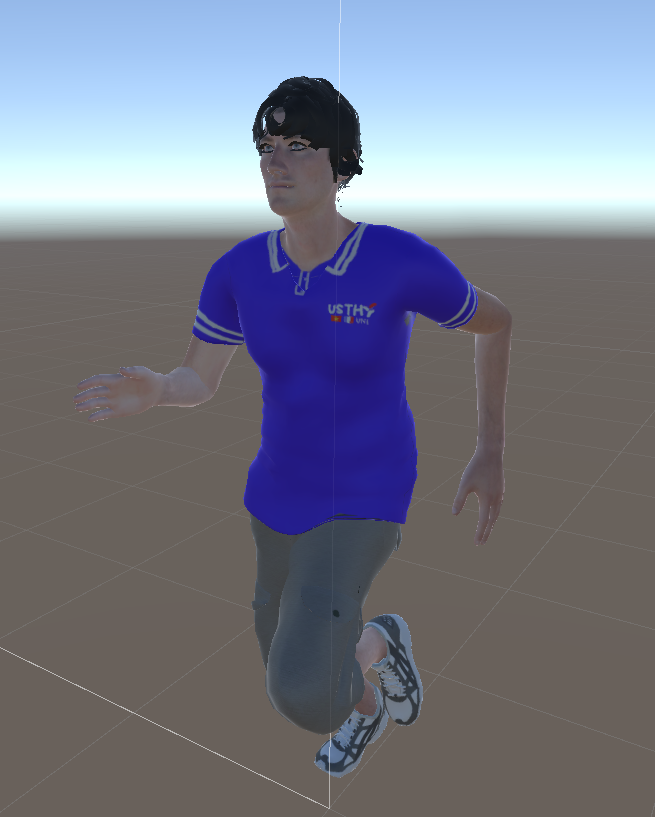
\includegraphics[width=0.4\textwidth]{front.png}
    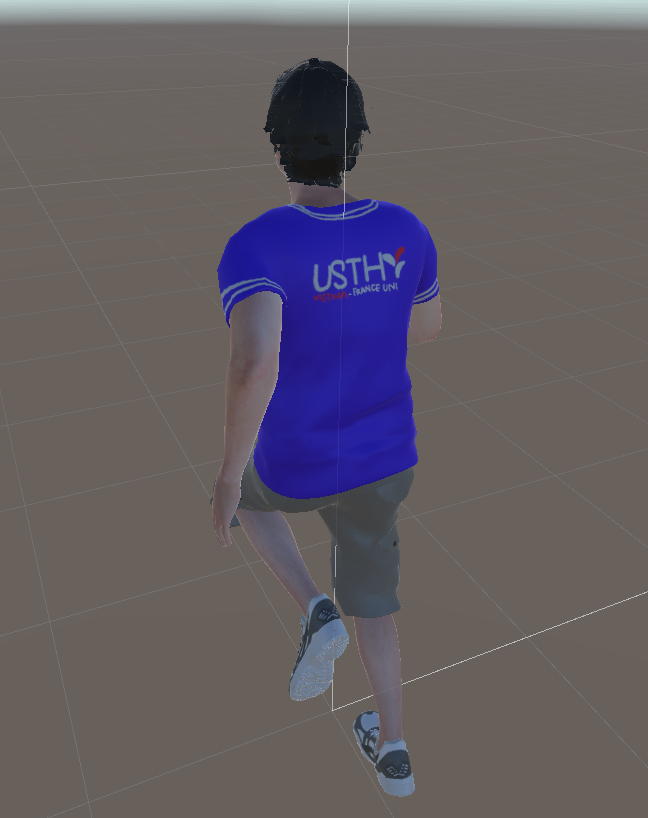
\includegraphics[width=0.4\textwidth]{back.png}
    \caption{Player Model.}
\end{figure}
With the animation from Mixamo, the model can now do Idle Stand, Run, Turn Left, Turn Right, Jump, Roll Over (Slide) and Fall Behind for the Endless-Running Game mode.

\clearpage
\subsubsection{Hallway Model}
Attempts were made to duplicate the USTH's 4th, 5th and 6th floor Hallway. There was a total of 5 hallways built: 2 In-between, and 1 for each floor of 4th, 5th and 6th.
\begin{figure}[H]
    \centering
    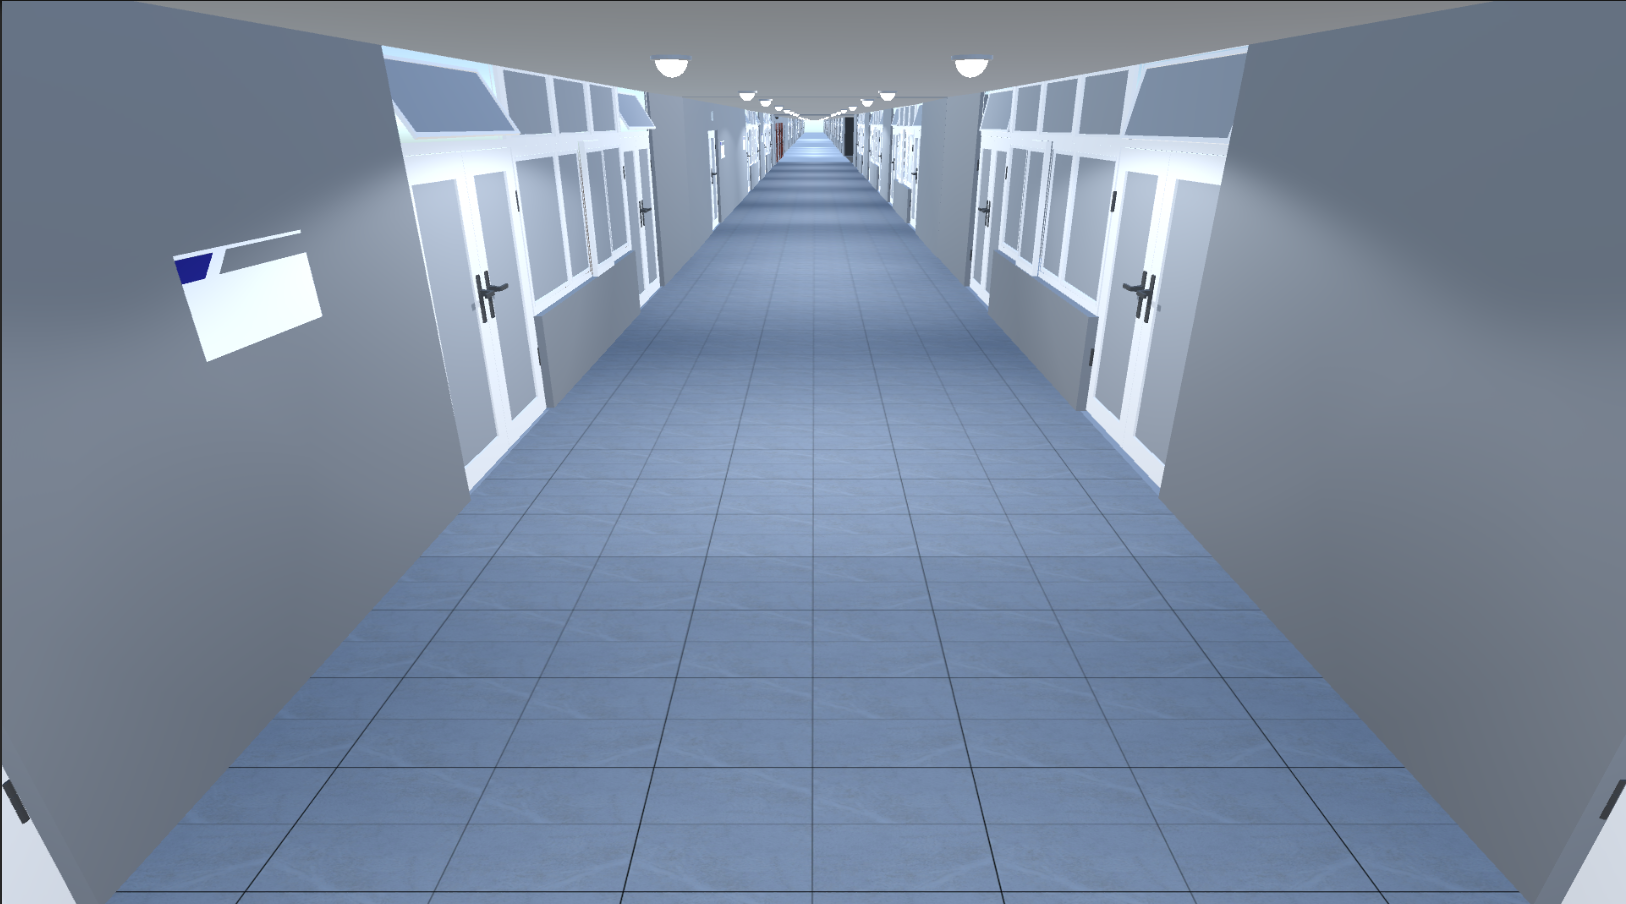
\includegraphics[width=0.54\textwidth]{f3.png}
    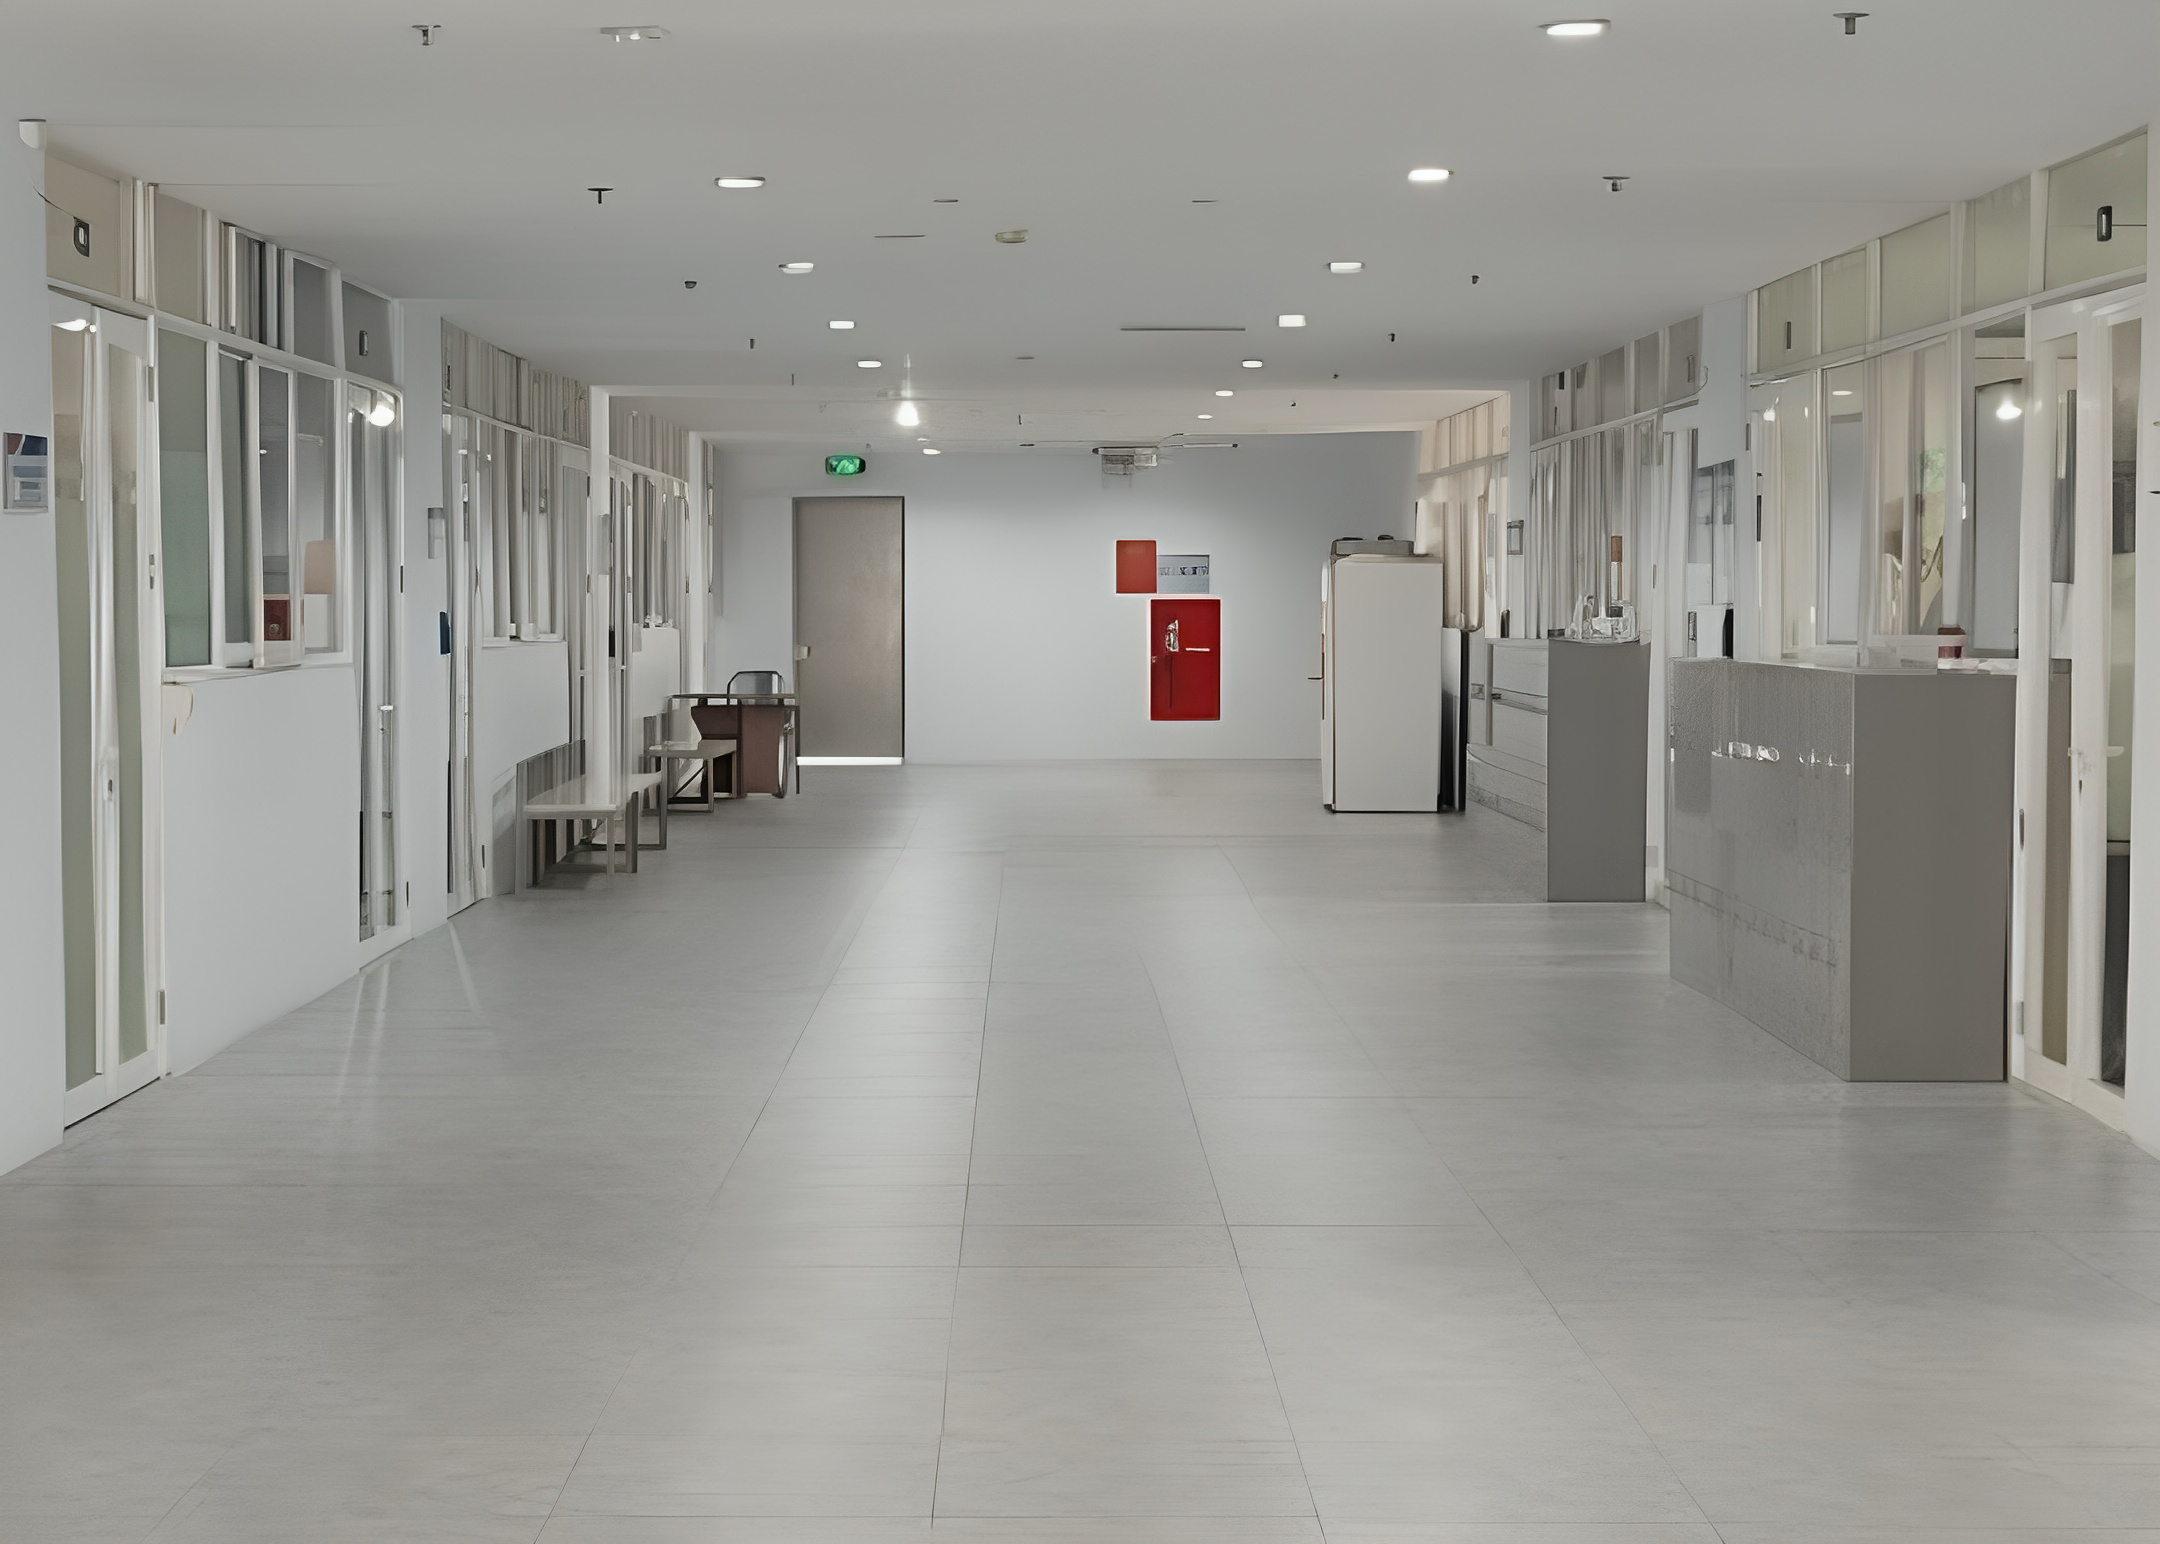
\includegraphics[width=0.44\textwidth]{hallway.png}
    \caption{In-between Hallways with Comparison.}
\end{figure}
\begin{figure}[H]
    \centering
    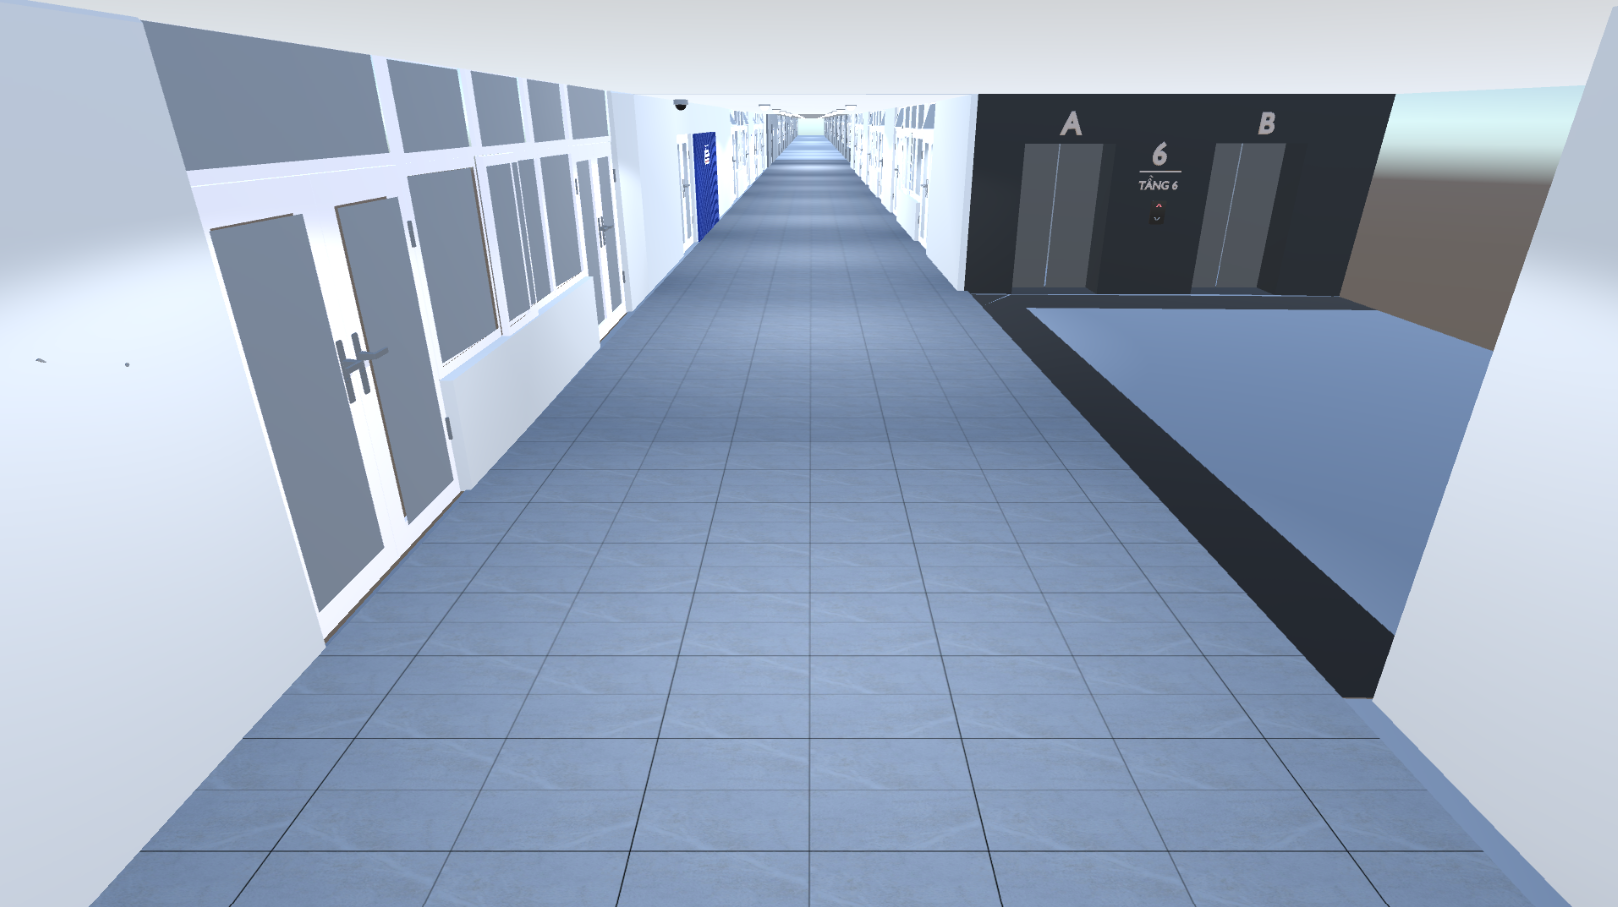
\includegraphics[width=0.54\textwidth]{f1.png}
    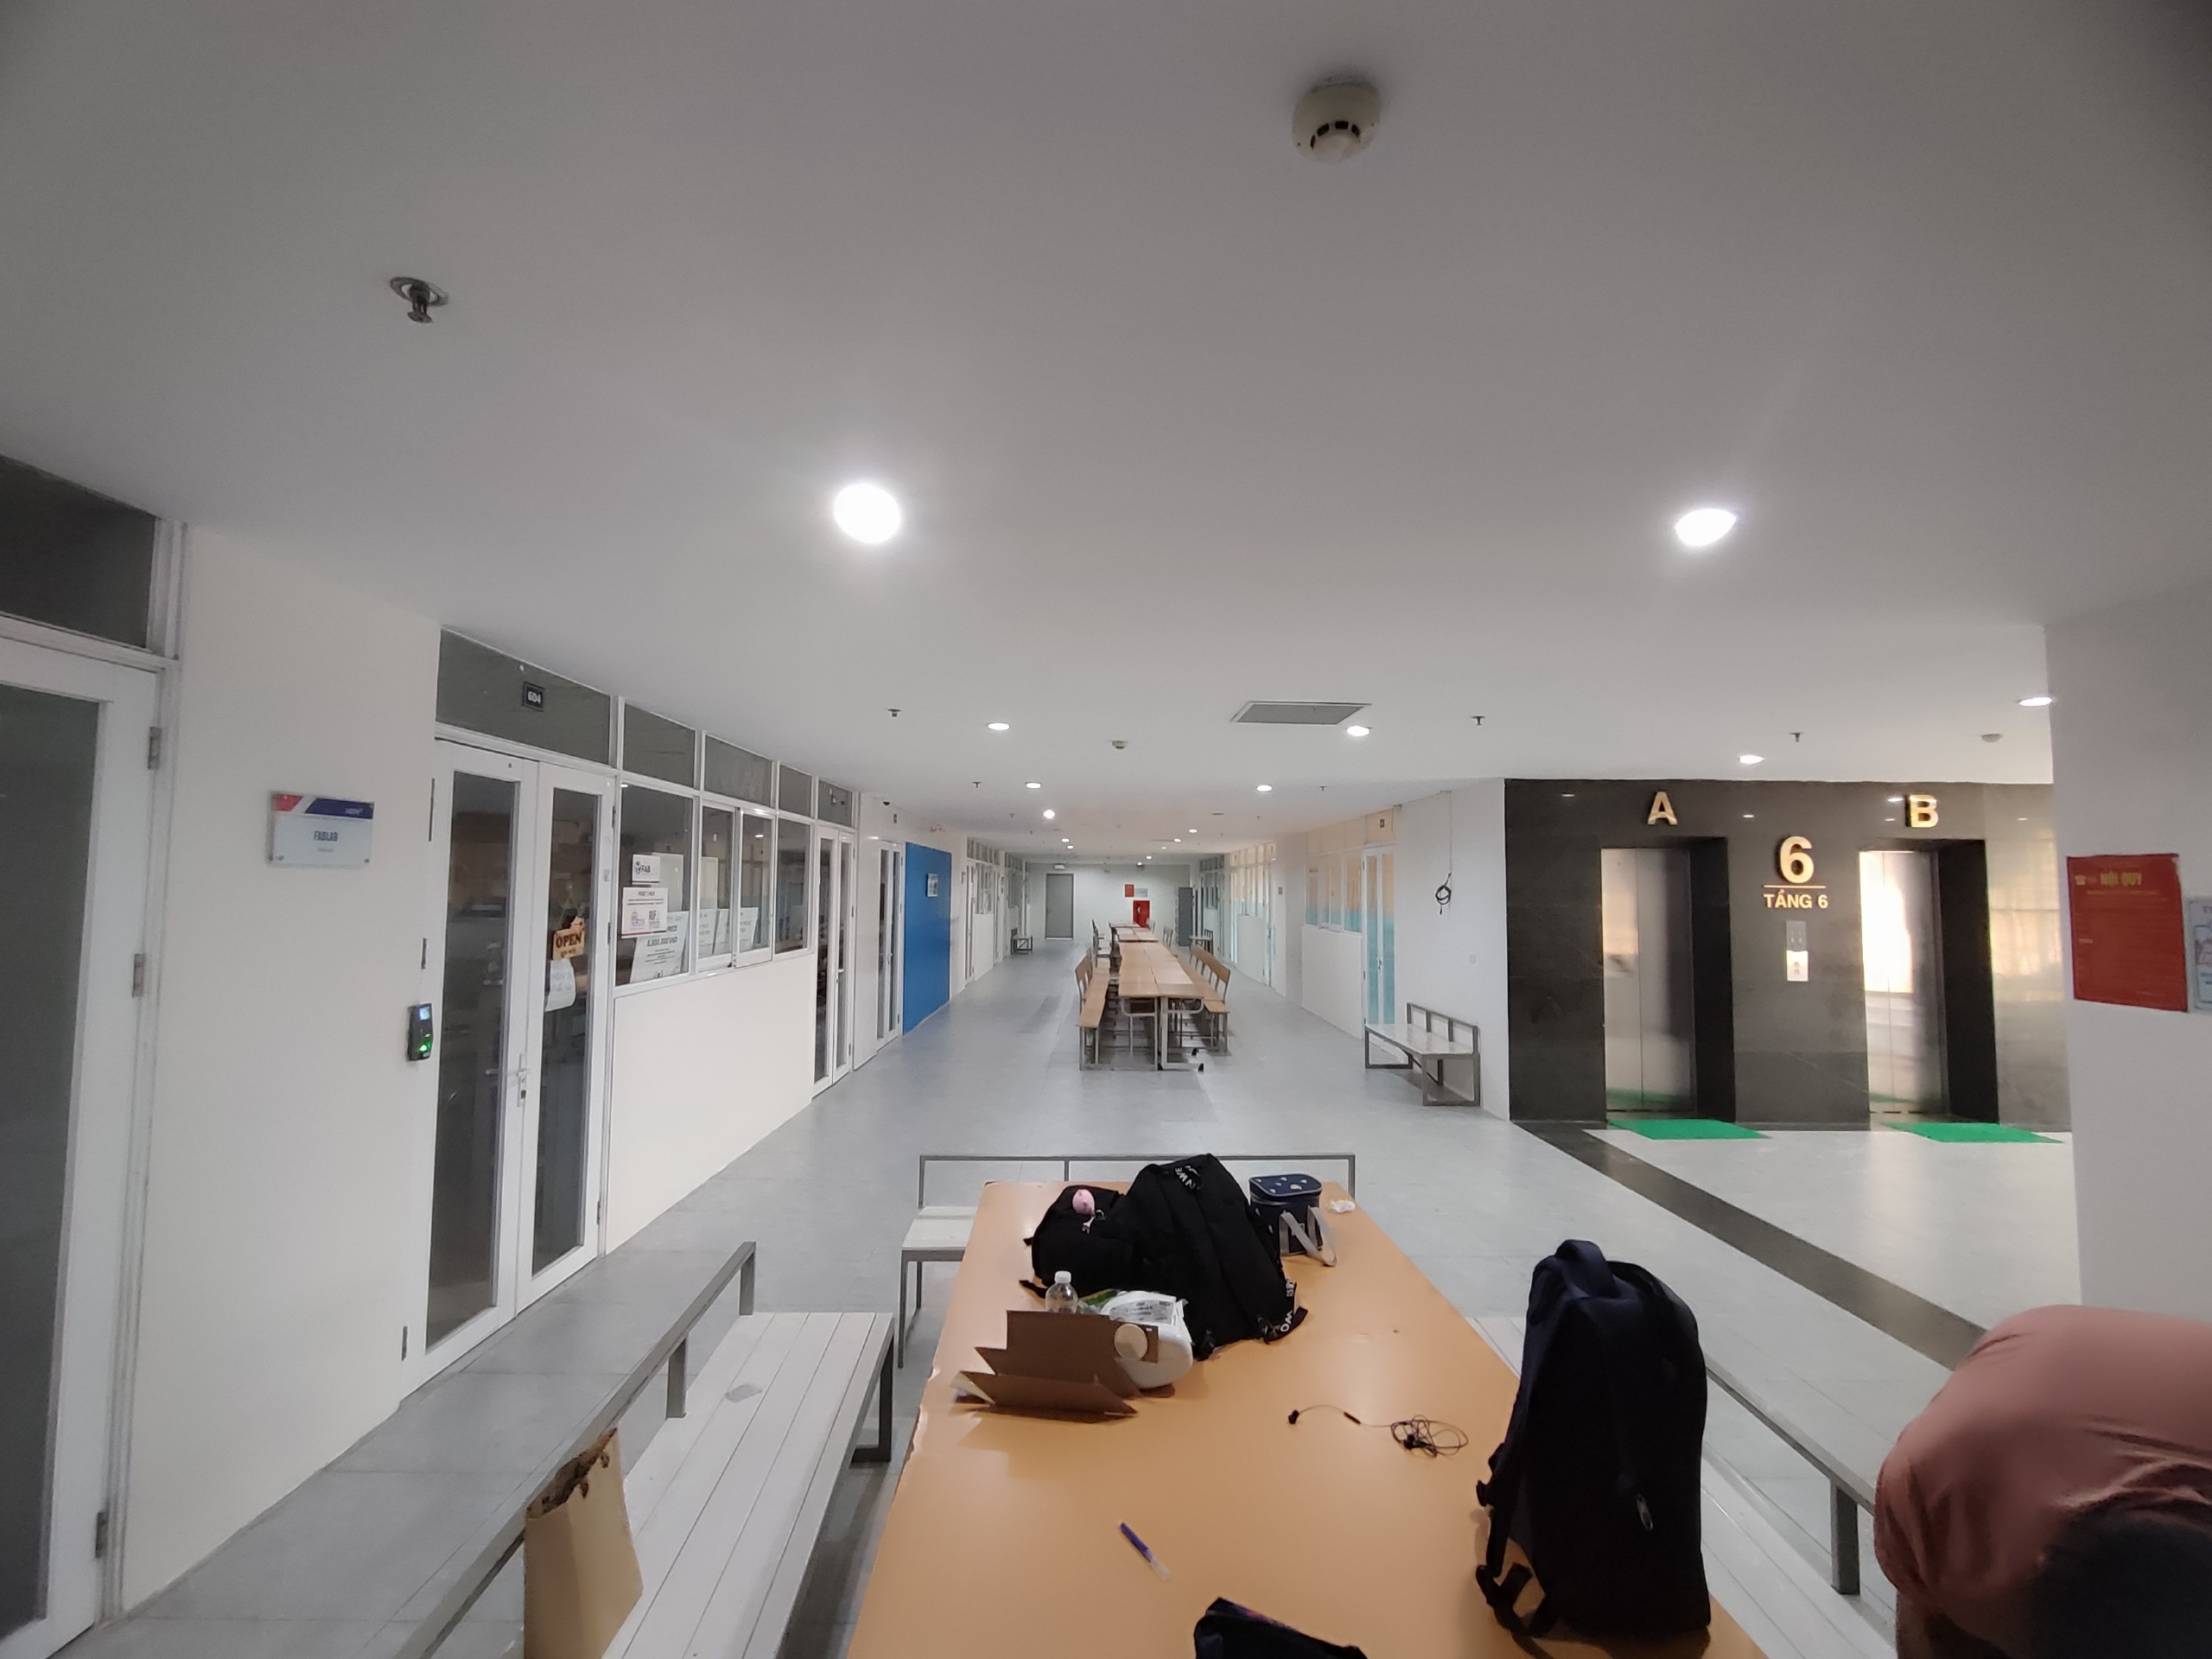
\includegraphics[width=0.44\textwidth]{t6.jpg}
    \caption{6th floor Hallways with Comparison.}
\end{figure}
\begin{figure}[H]
    \centering
    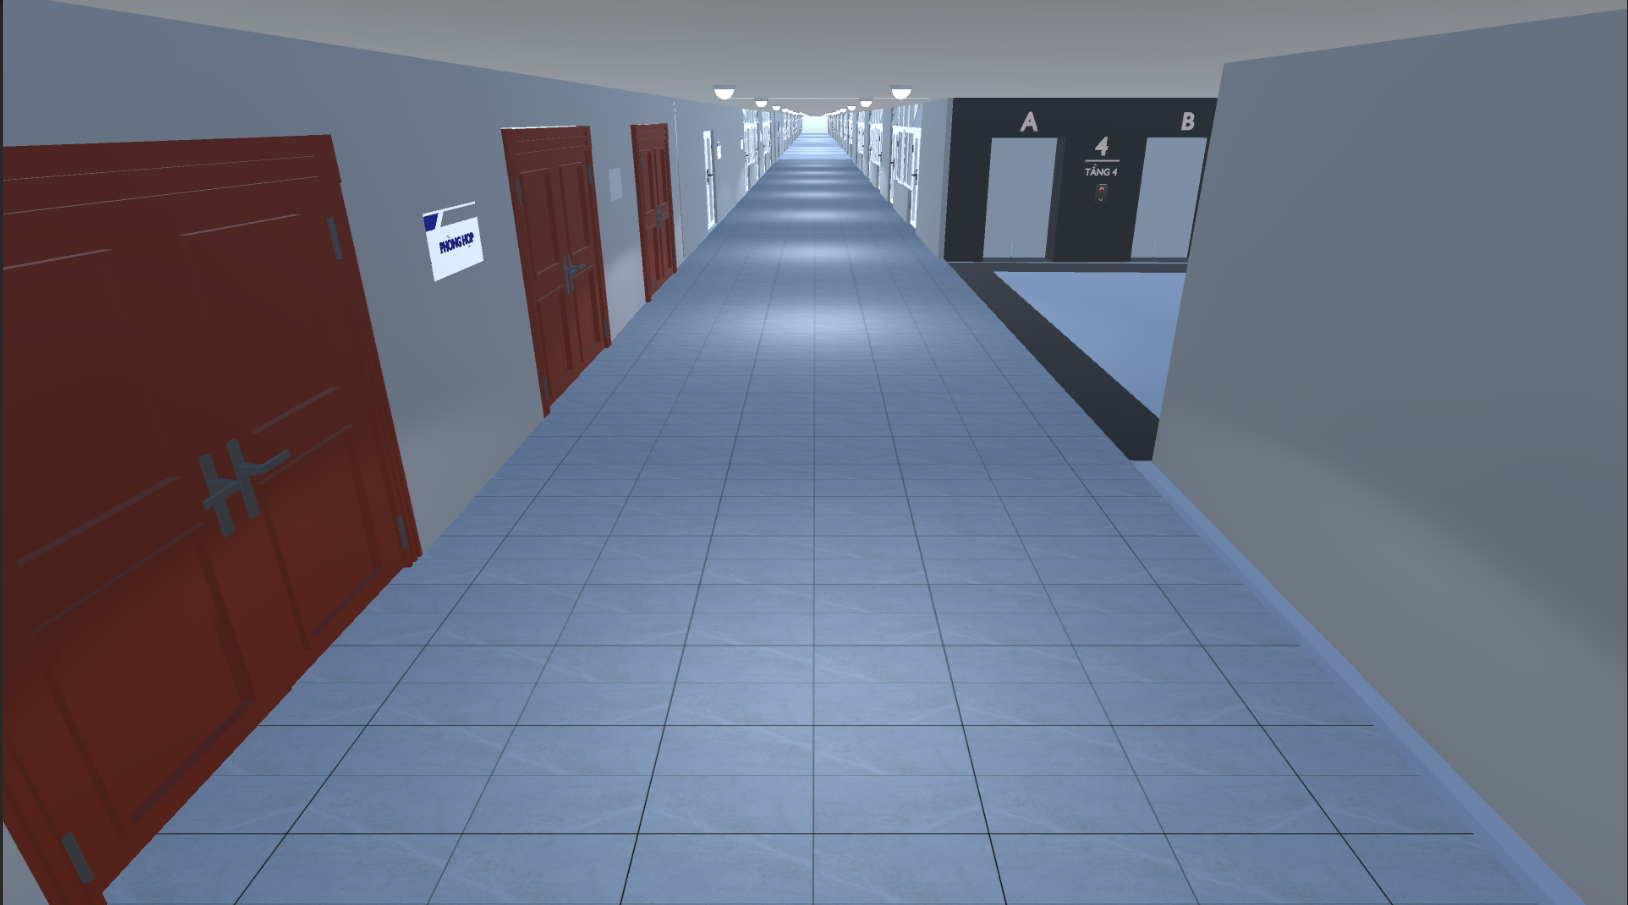
\includegraphics[width=0.54\textwidth]{f2.png}
    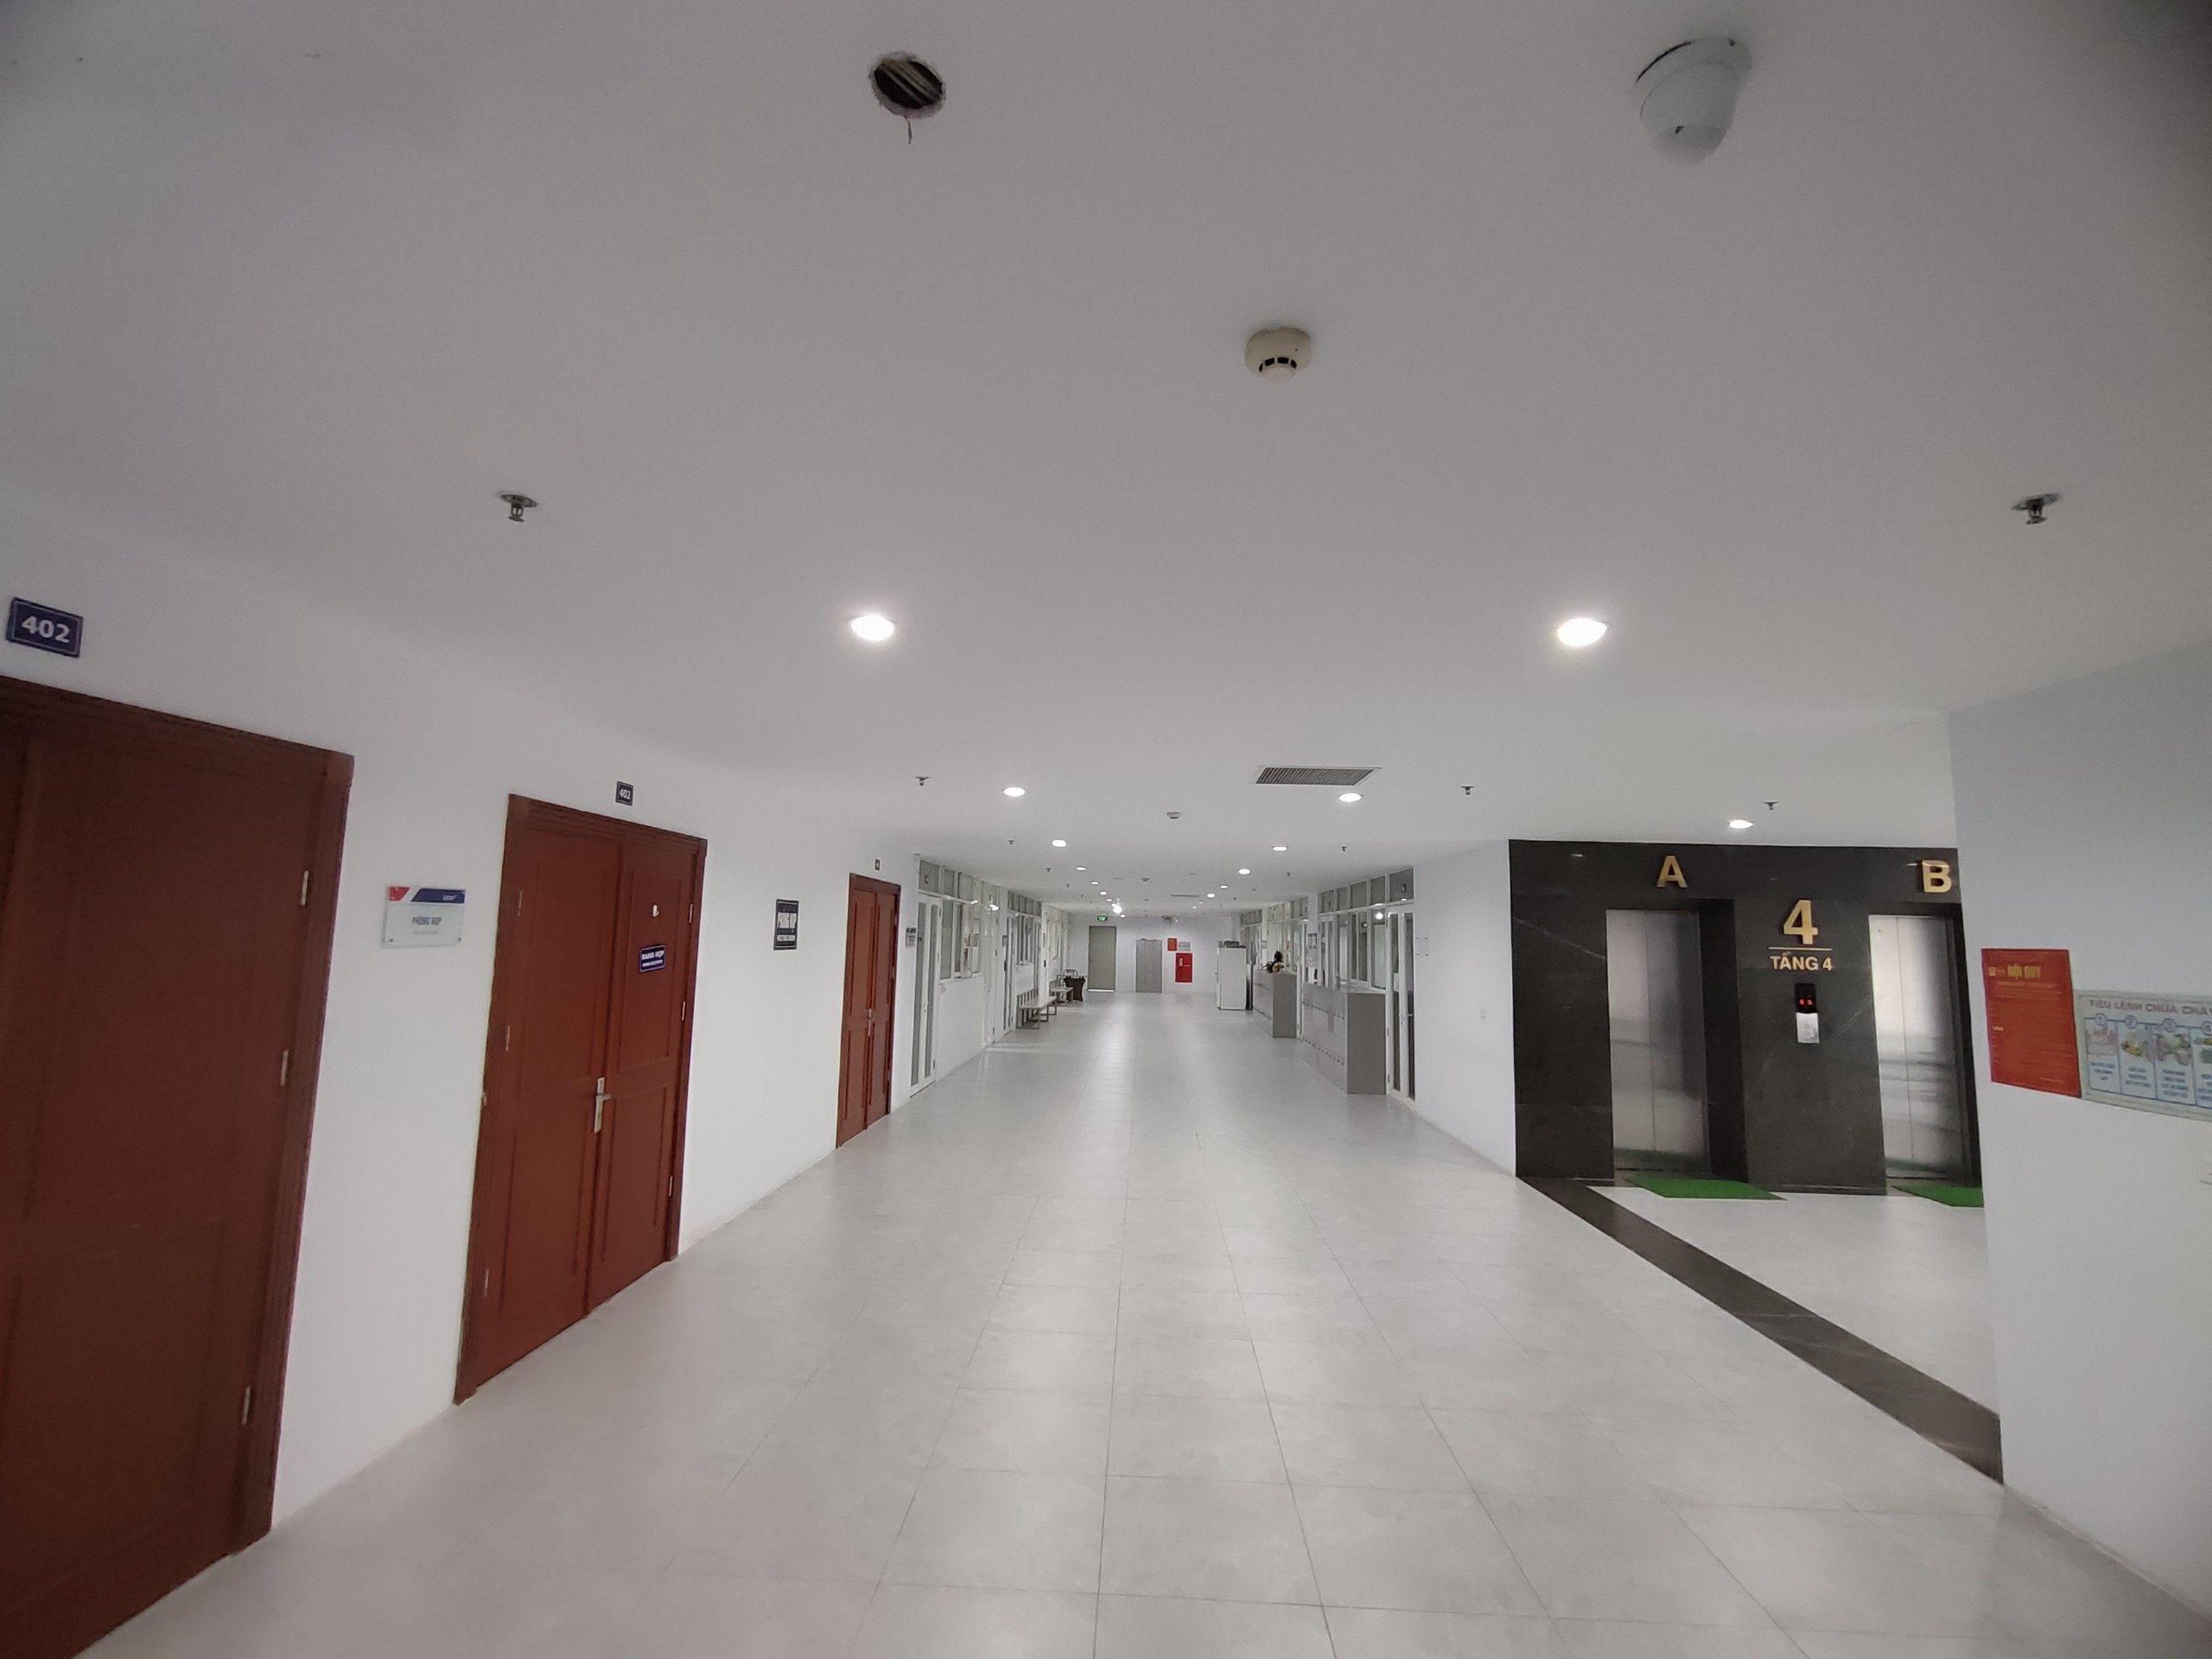
\includegraphics[width=0.44\textwidth]{t4.jpg}
    \caption{4th floor Hallways with Comparison.}
\end{figure}
\clearpage
\subsubsection{Object Model}
The objects of the University are also made in Blender so that the game could have more of the USTH-vibe.
\begin{figure}[H]
    \centering
    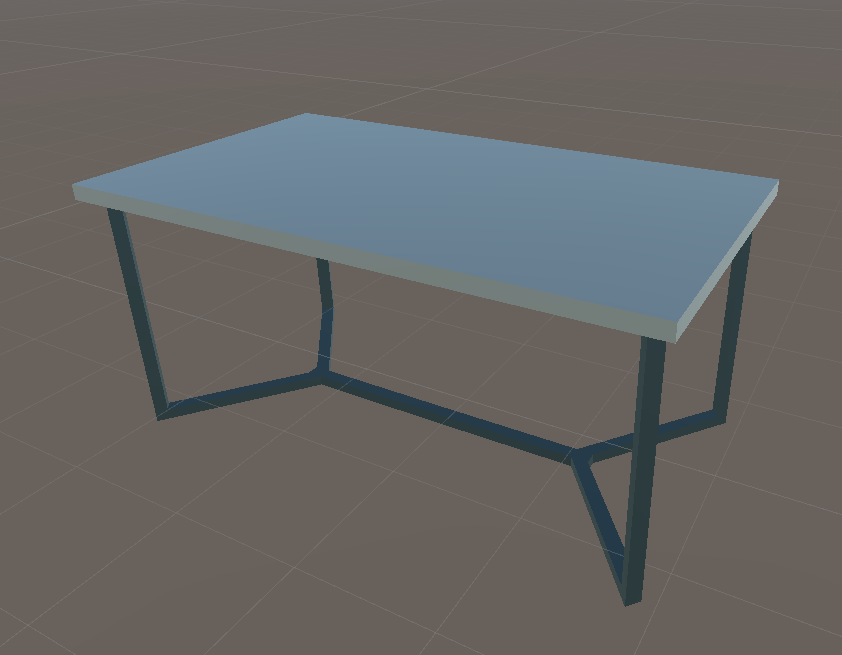
\includegraphics[width=0.49\textwidth]{o1.png}
    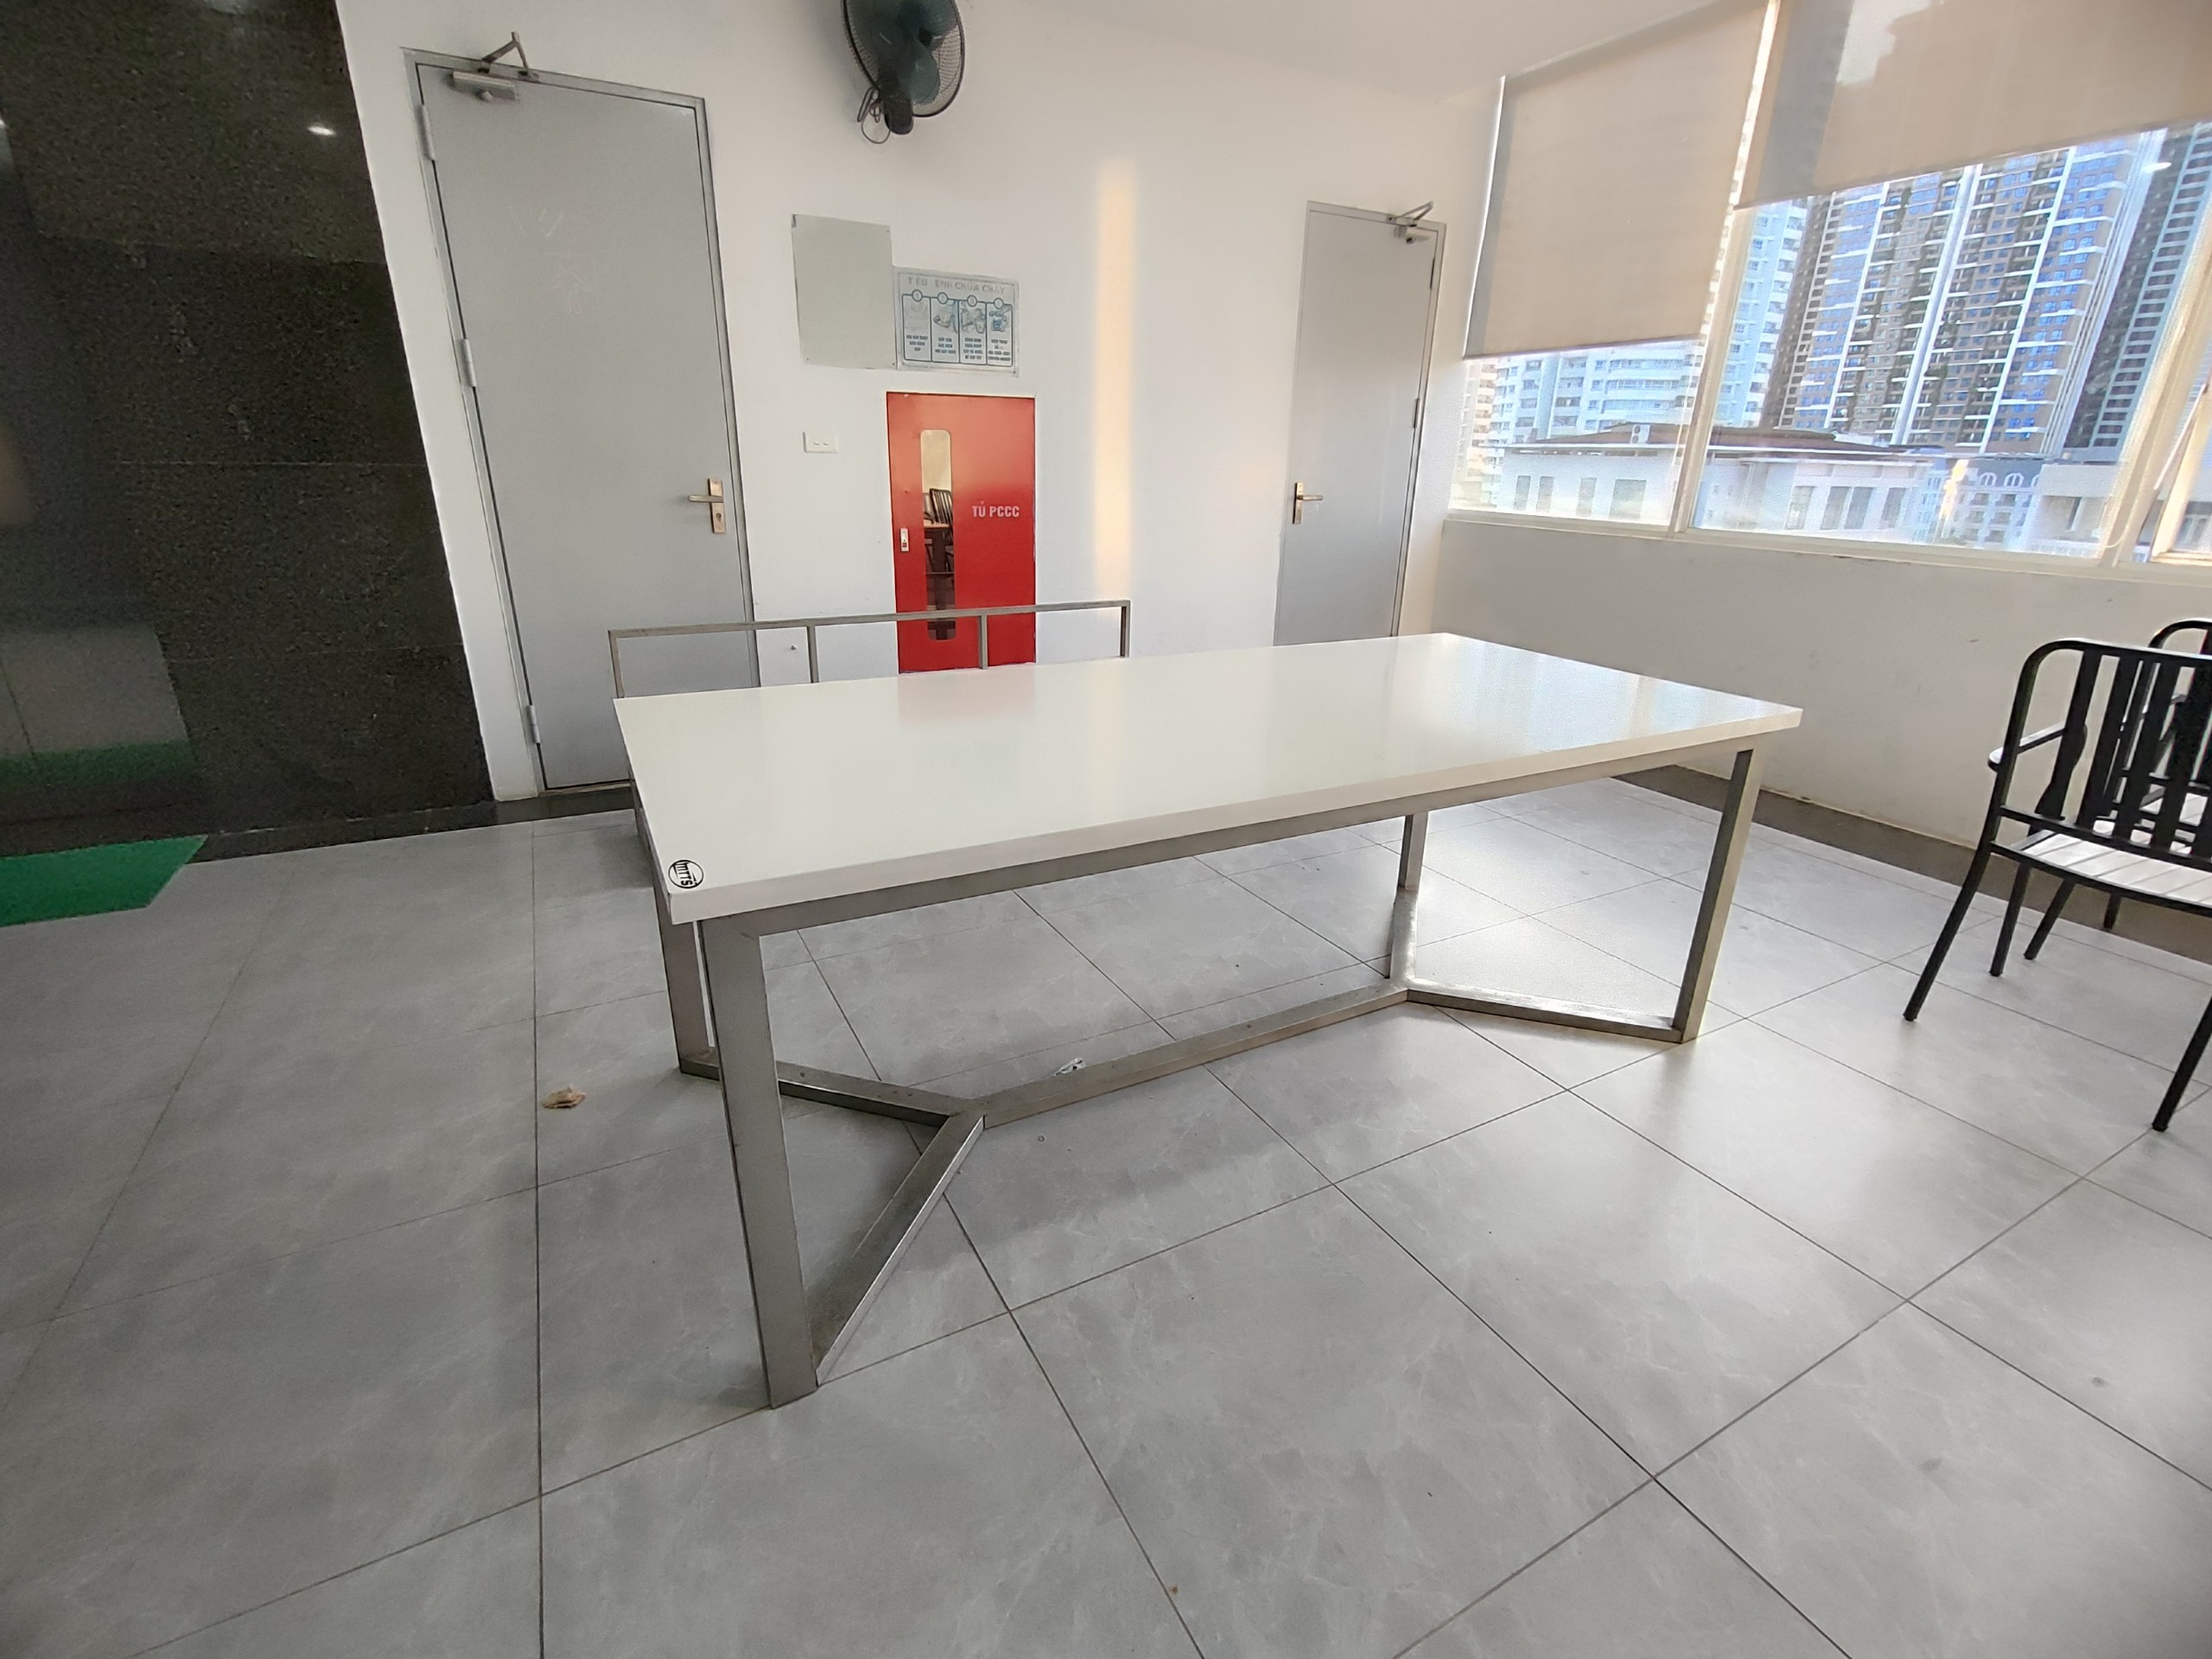
\includegraphics[width=0.49\textwidth]{ban.jpg}
    \caption{Big Table with Comparison.}
\end{figure}

\begin{figure}[H]
    \centering
    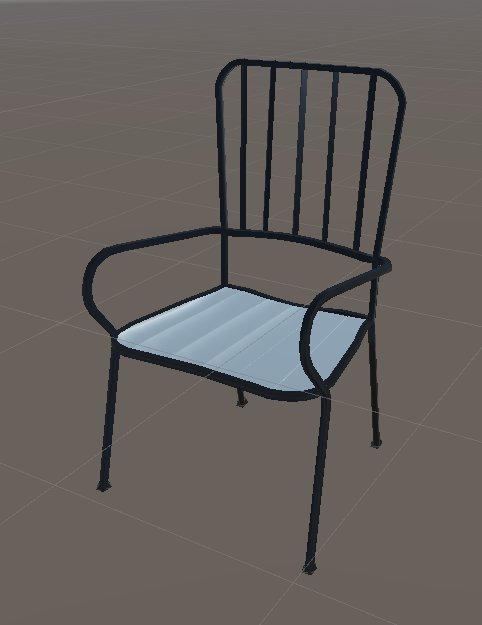
\includegraphics[width=0.49\textwidth]{o2.png}
    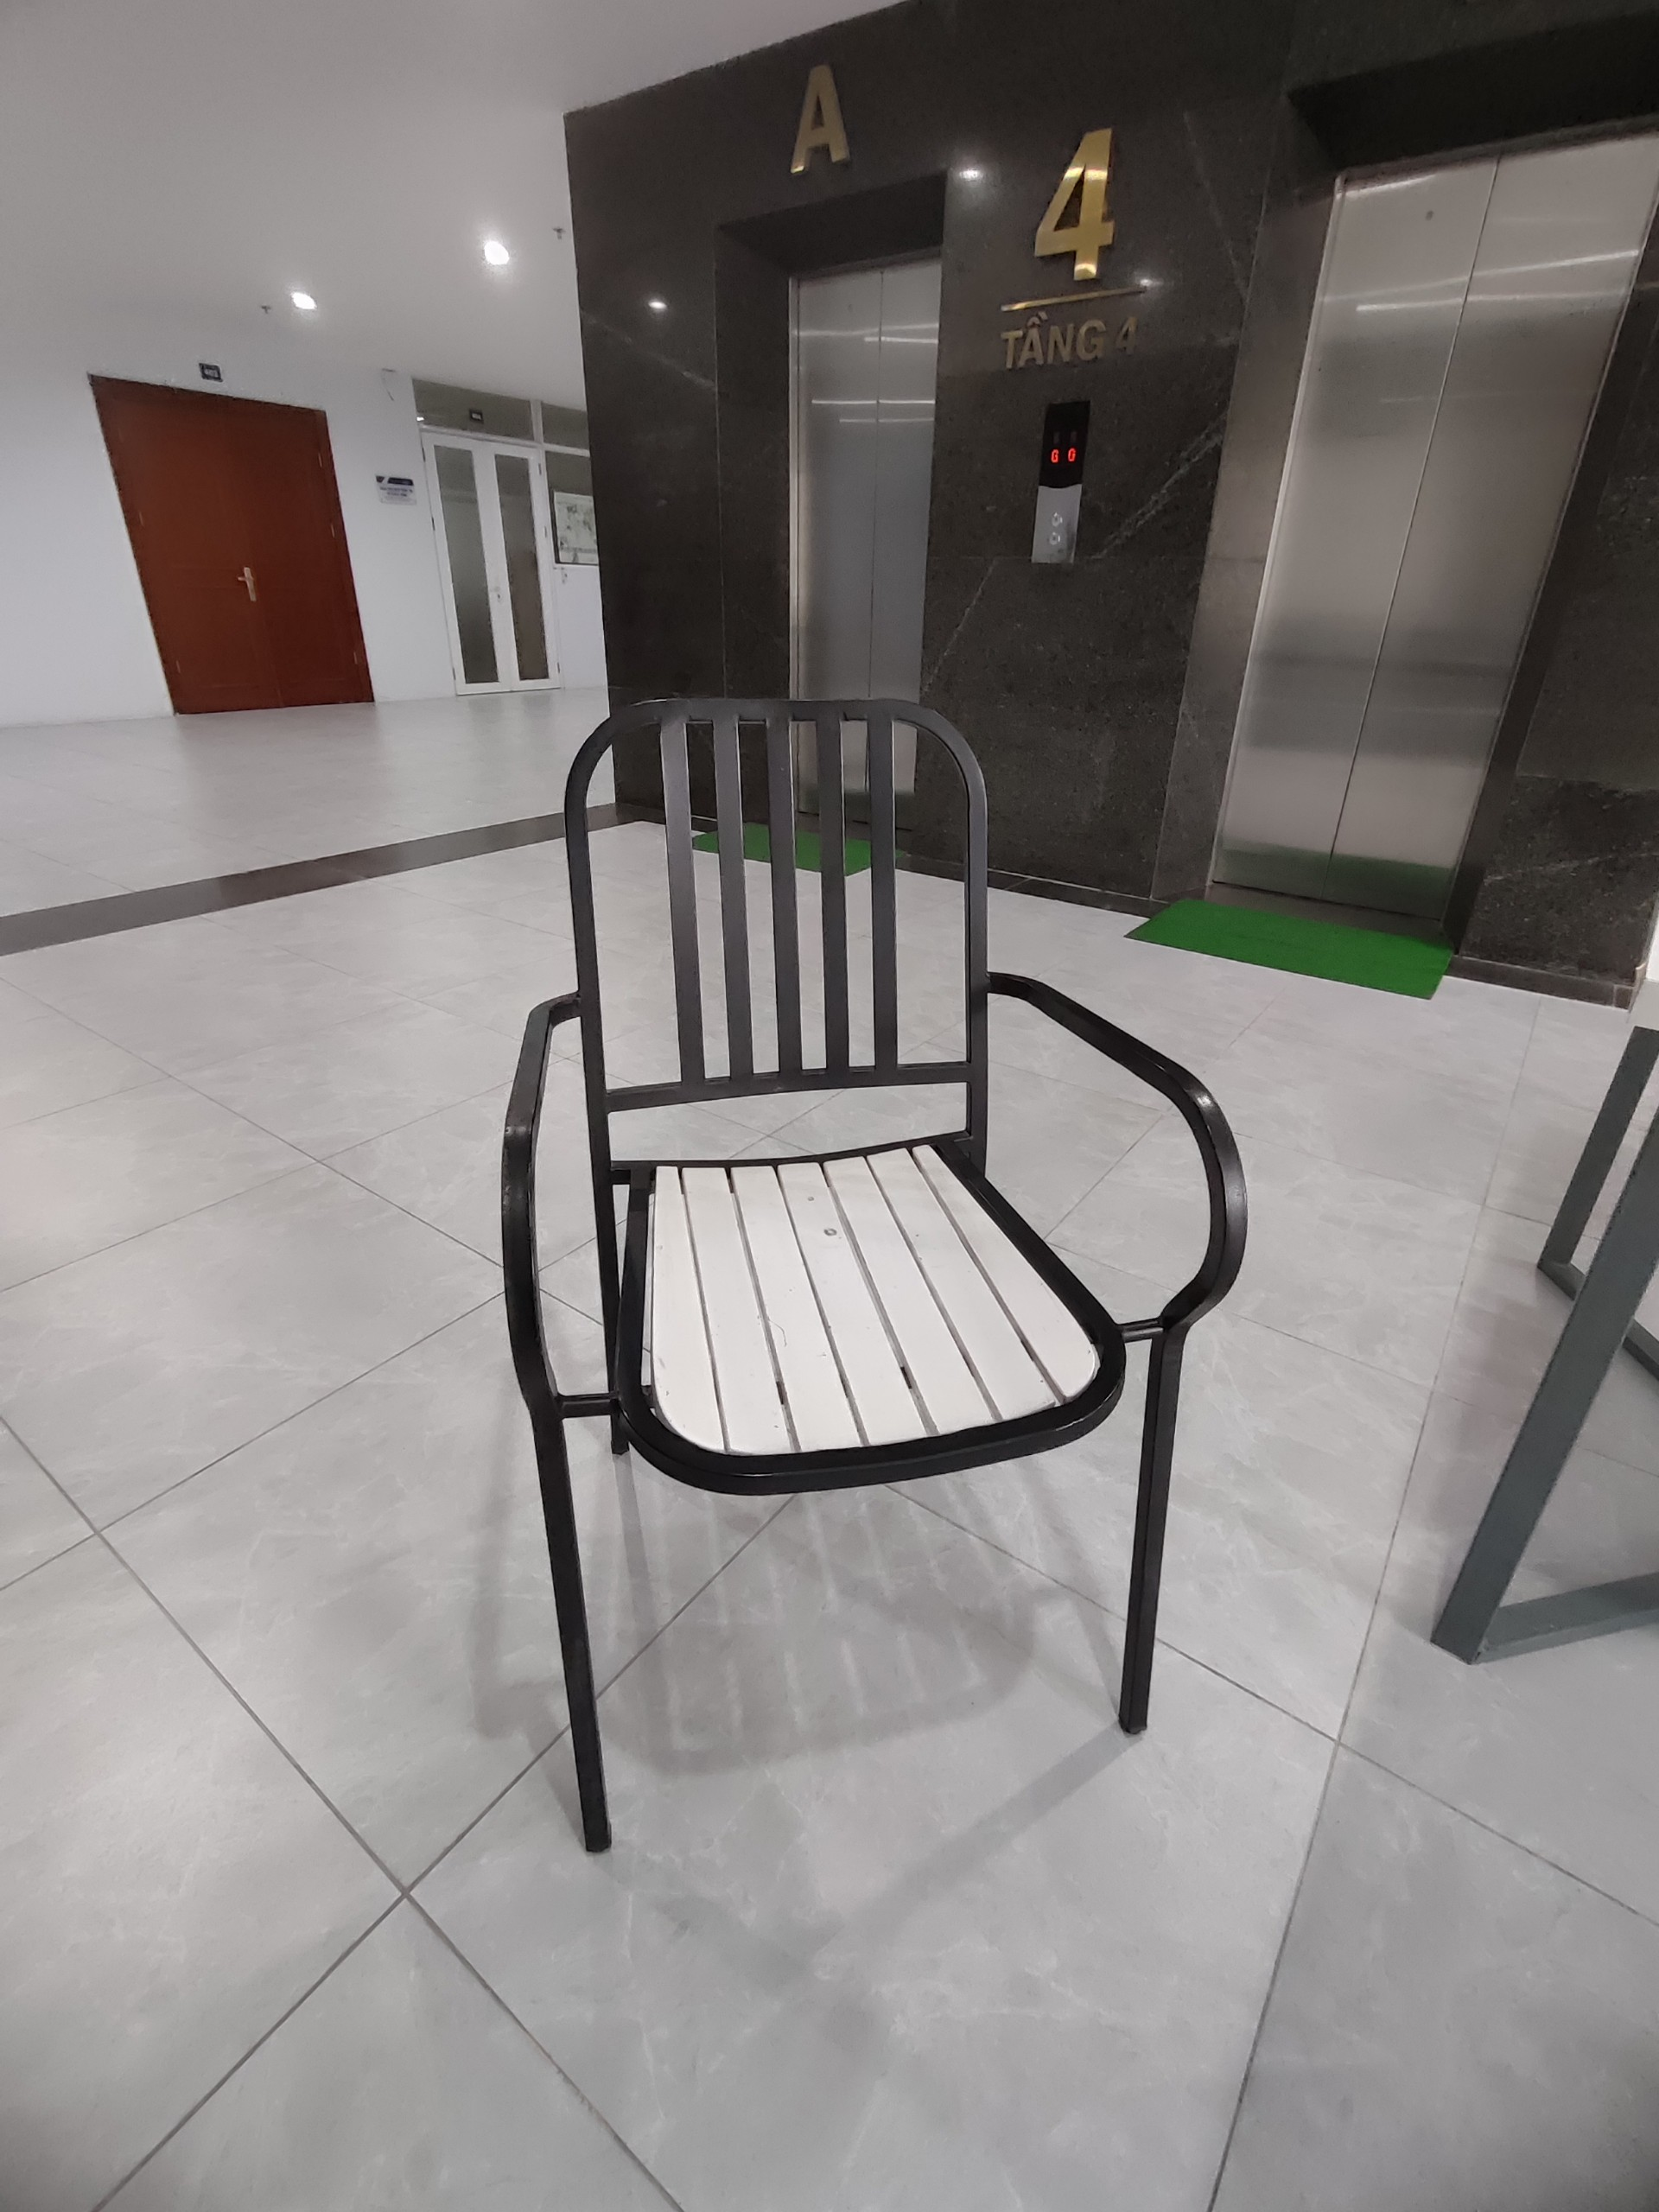
\includegraphics[width=0.49\textwidth]{4chan.jpg}
    \caption{Black Chair with Comparison.}
\end{figure}

\begin{figure}[H]
    \centering
    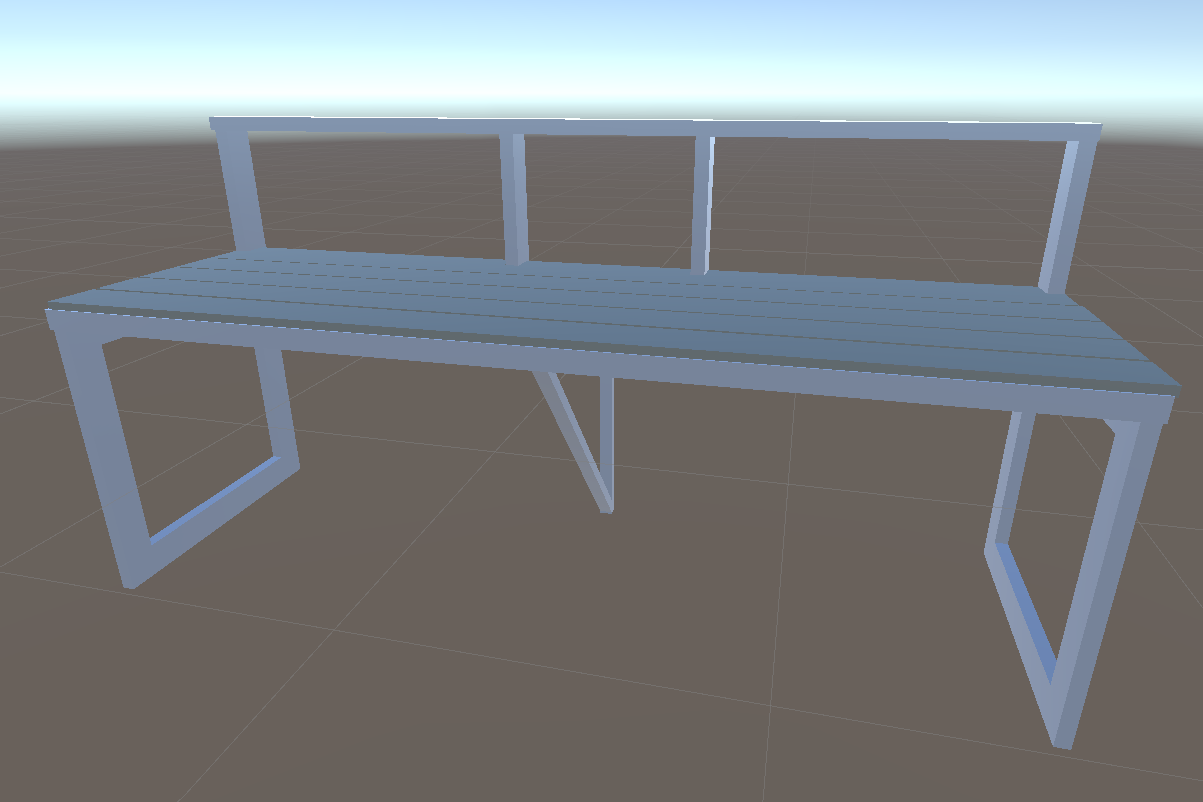
\includegraphics[width=0.49\textwidth]{o3.png}
    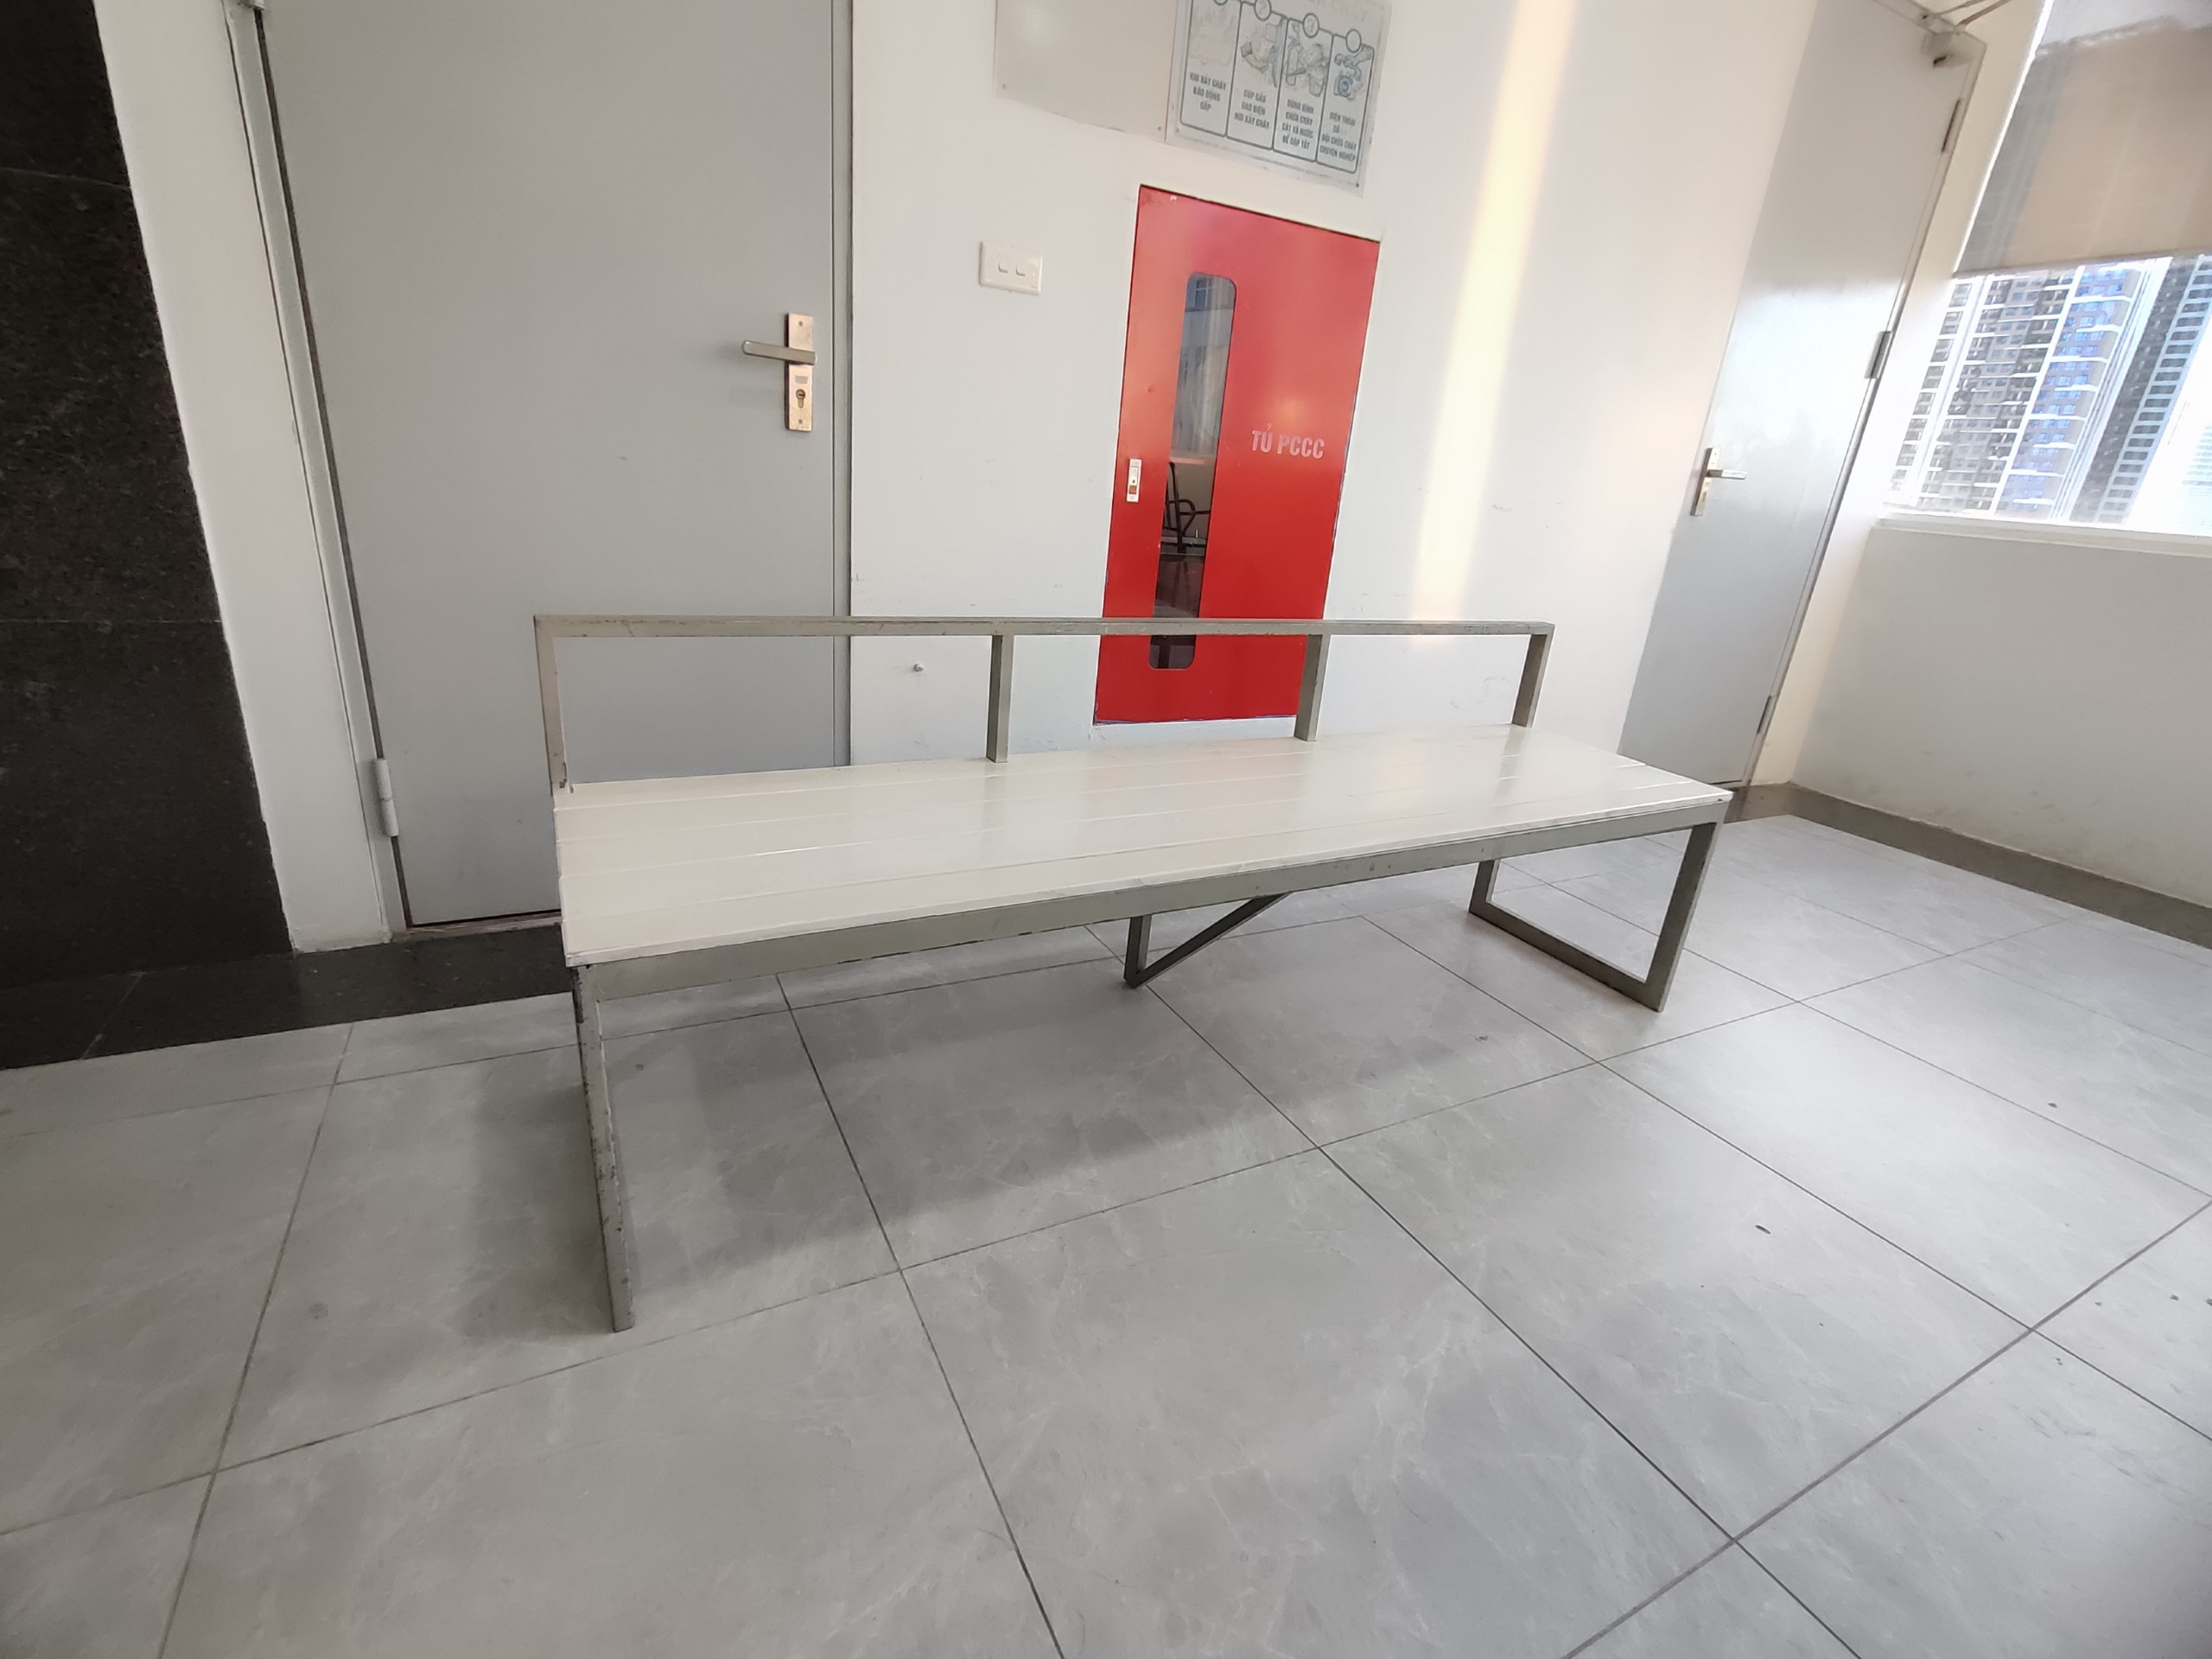
\includegraphics[width=0.49\textwidth]{ghe.jpg}
    \caption{Long Chair with Comparison.}
\end{figure}

\begin{figure}[H]
    \centering
    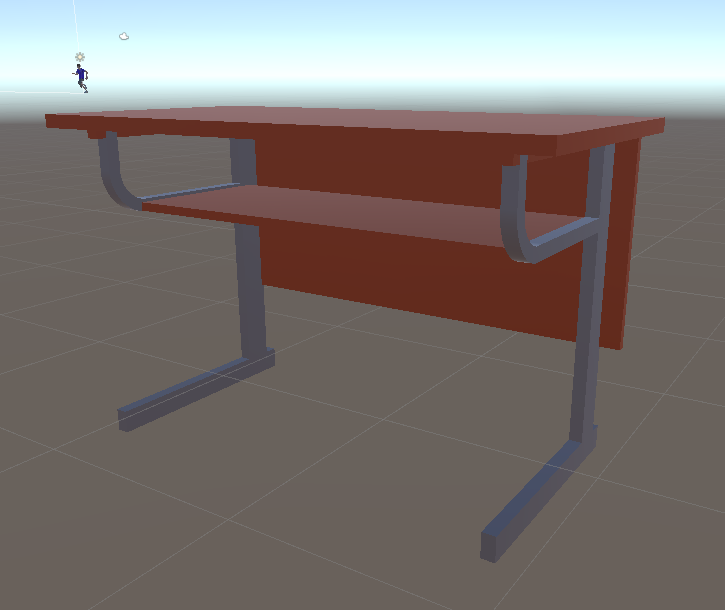
\includegraphics[width=0.49\textwidth]{o5.png}
    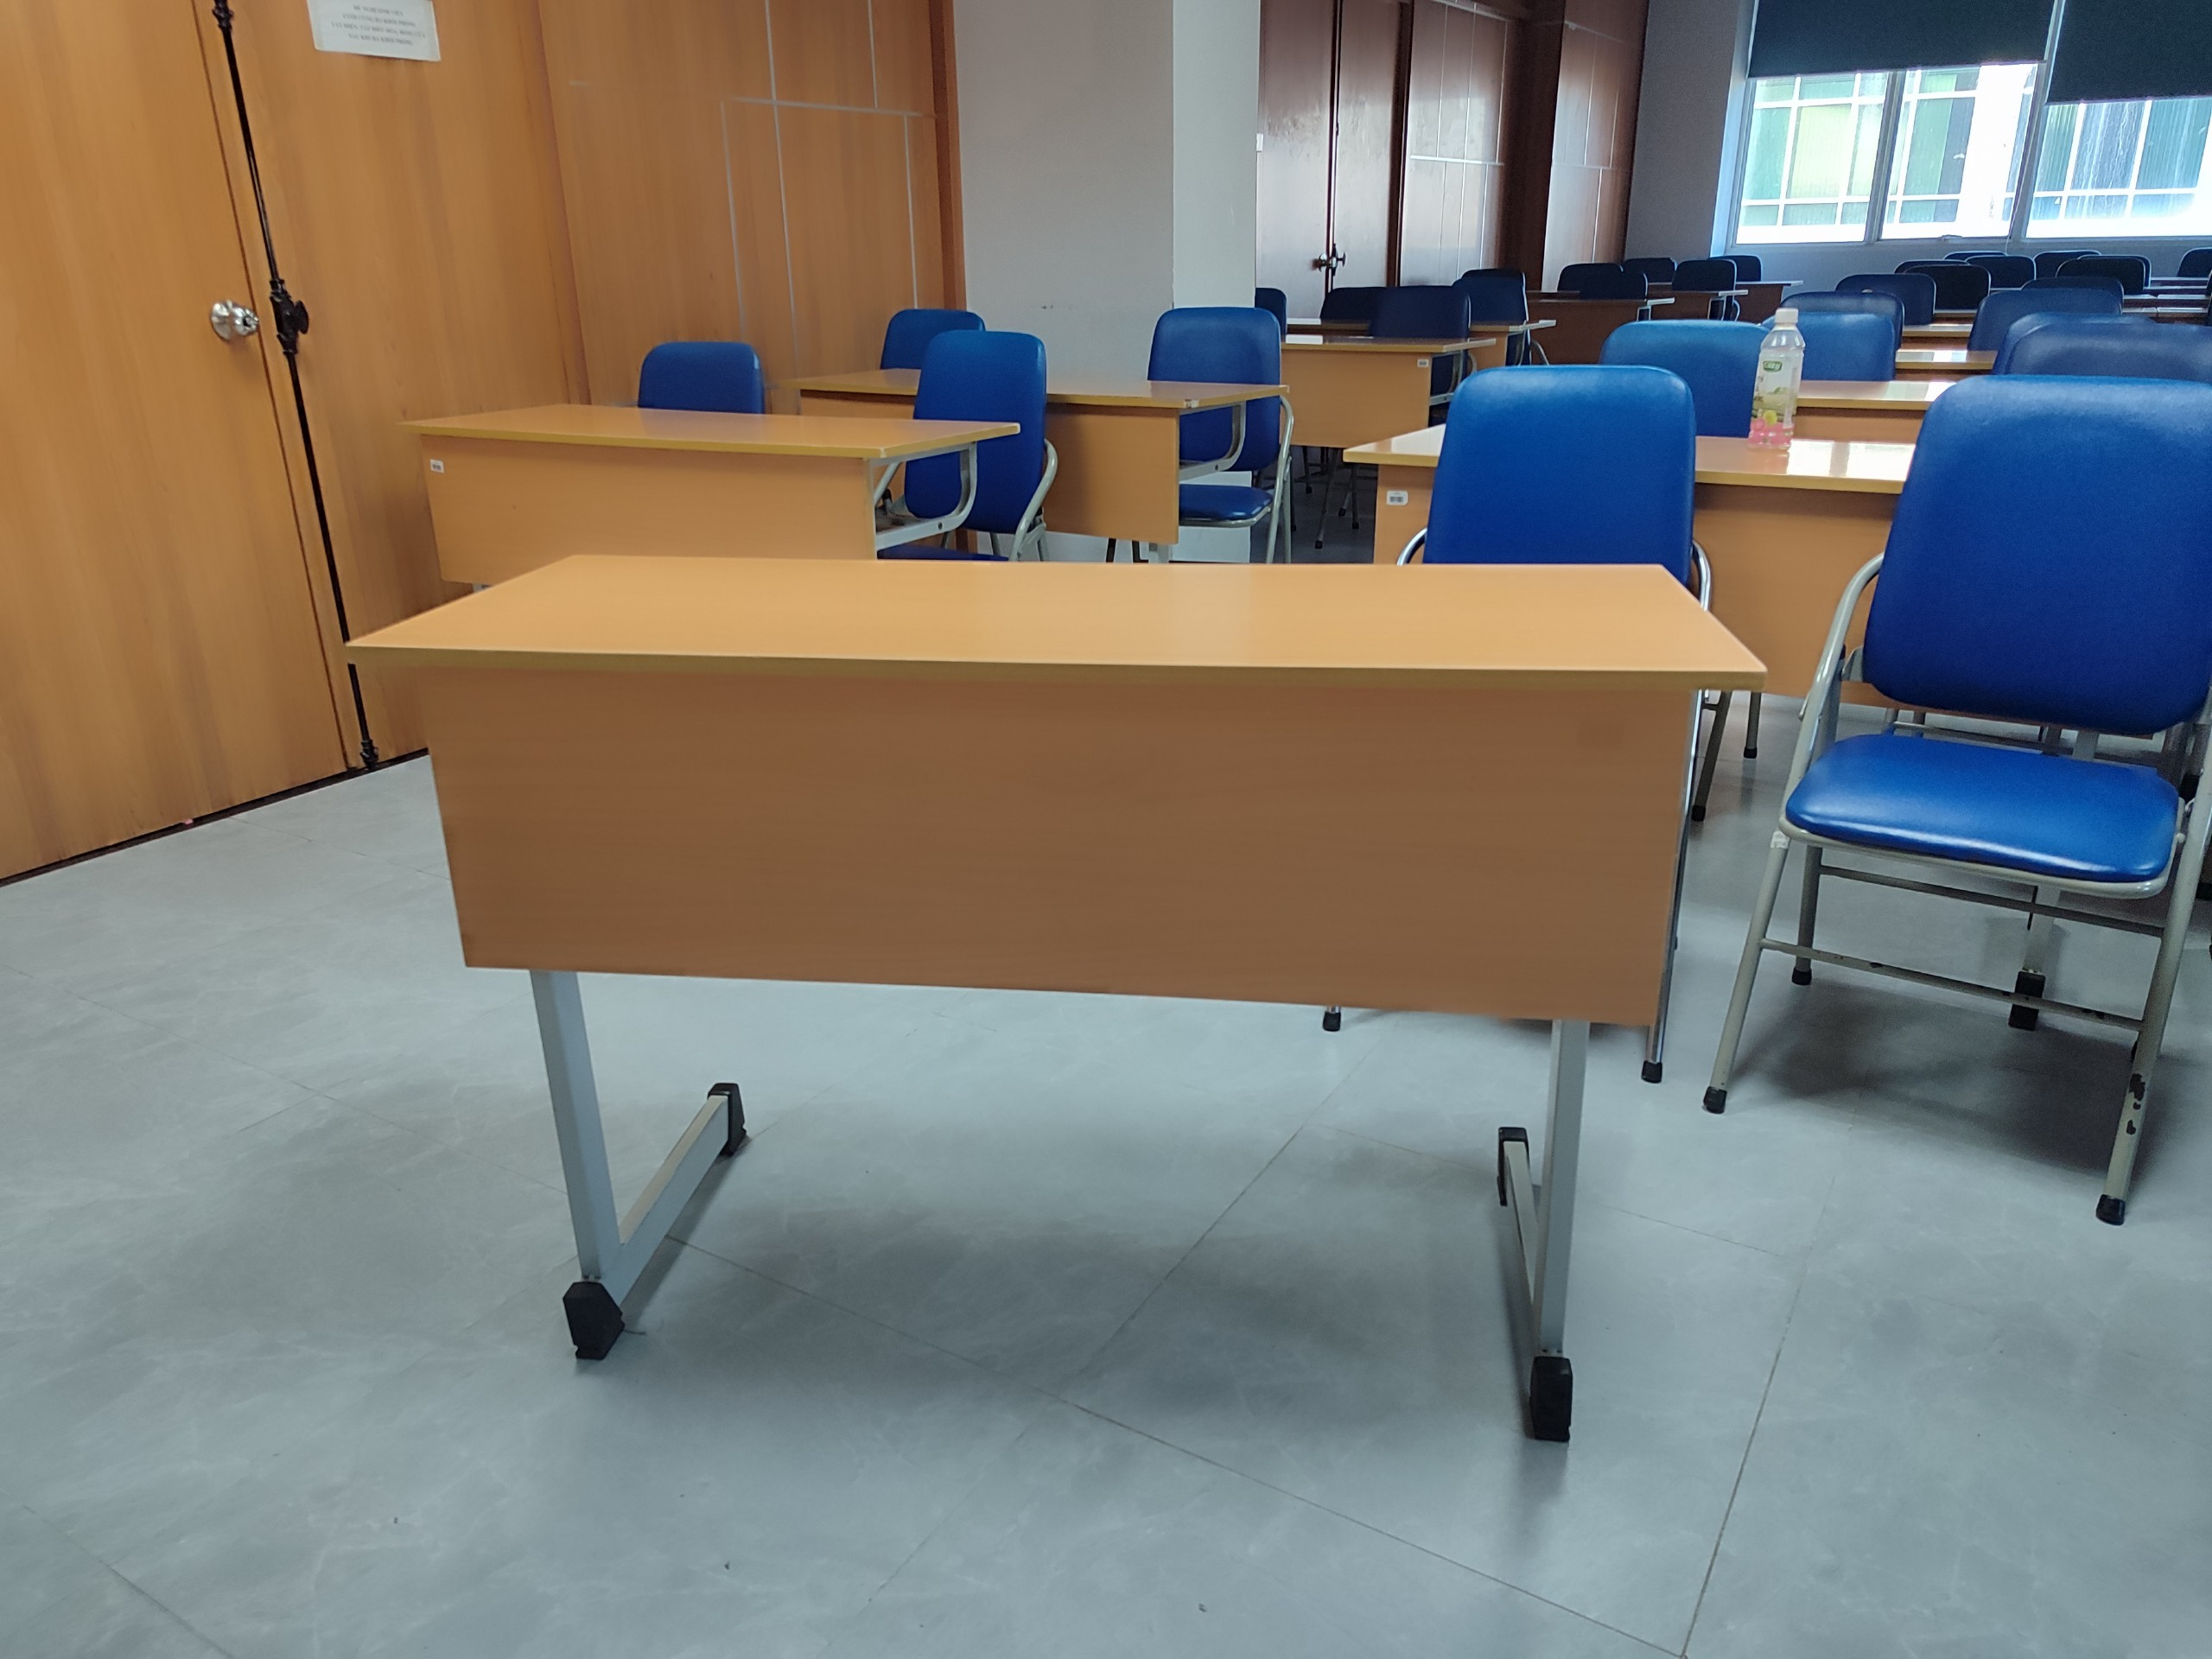
\includegraphics[width=0.49\textwidth]{go.jpg}
    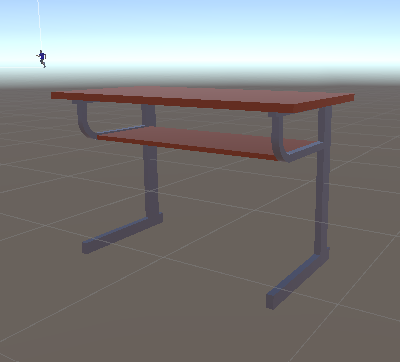
\includegraphics[width=0.49\textwidth]{o6.png}
    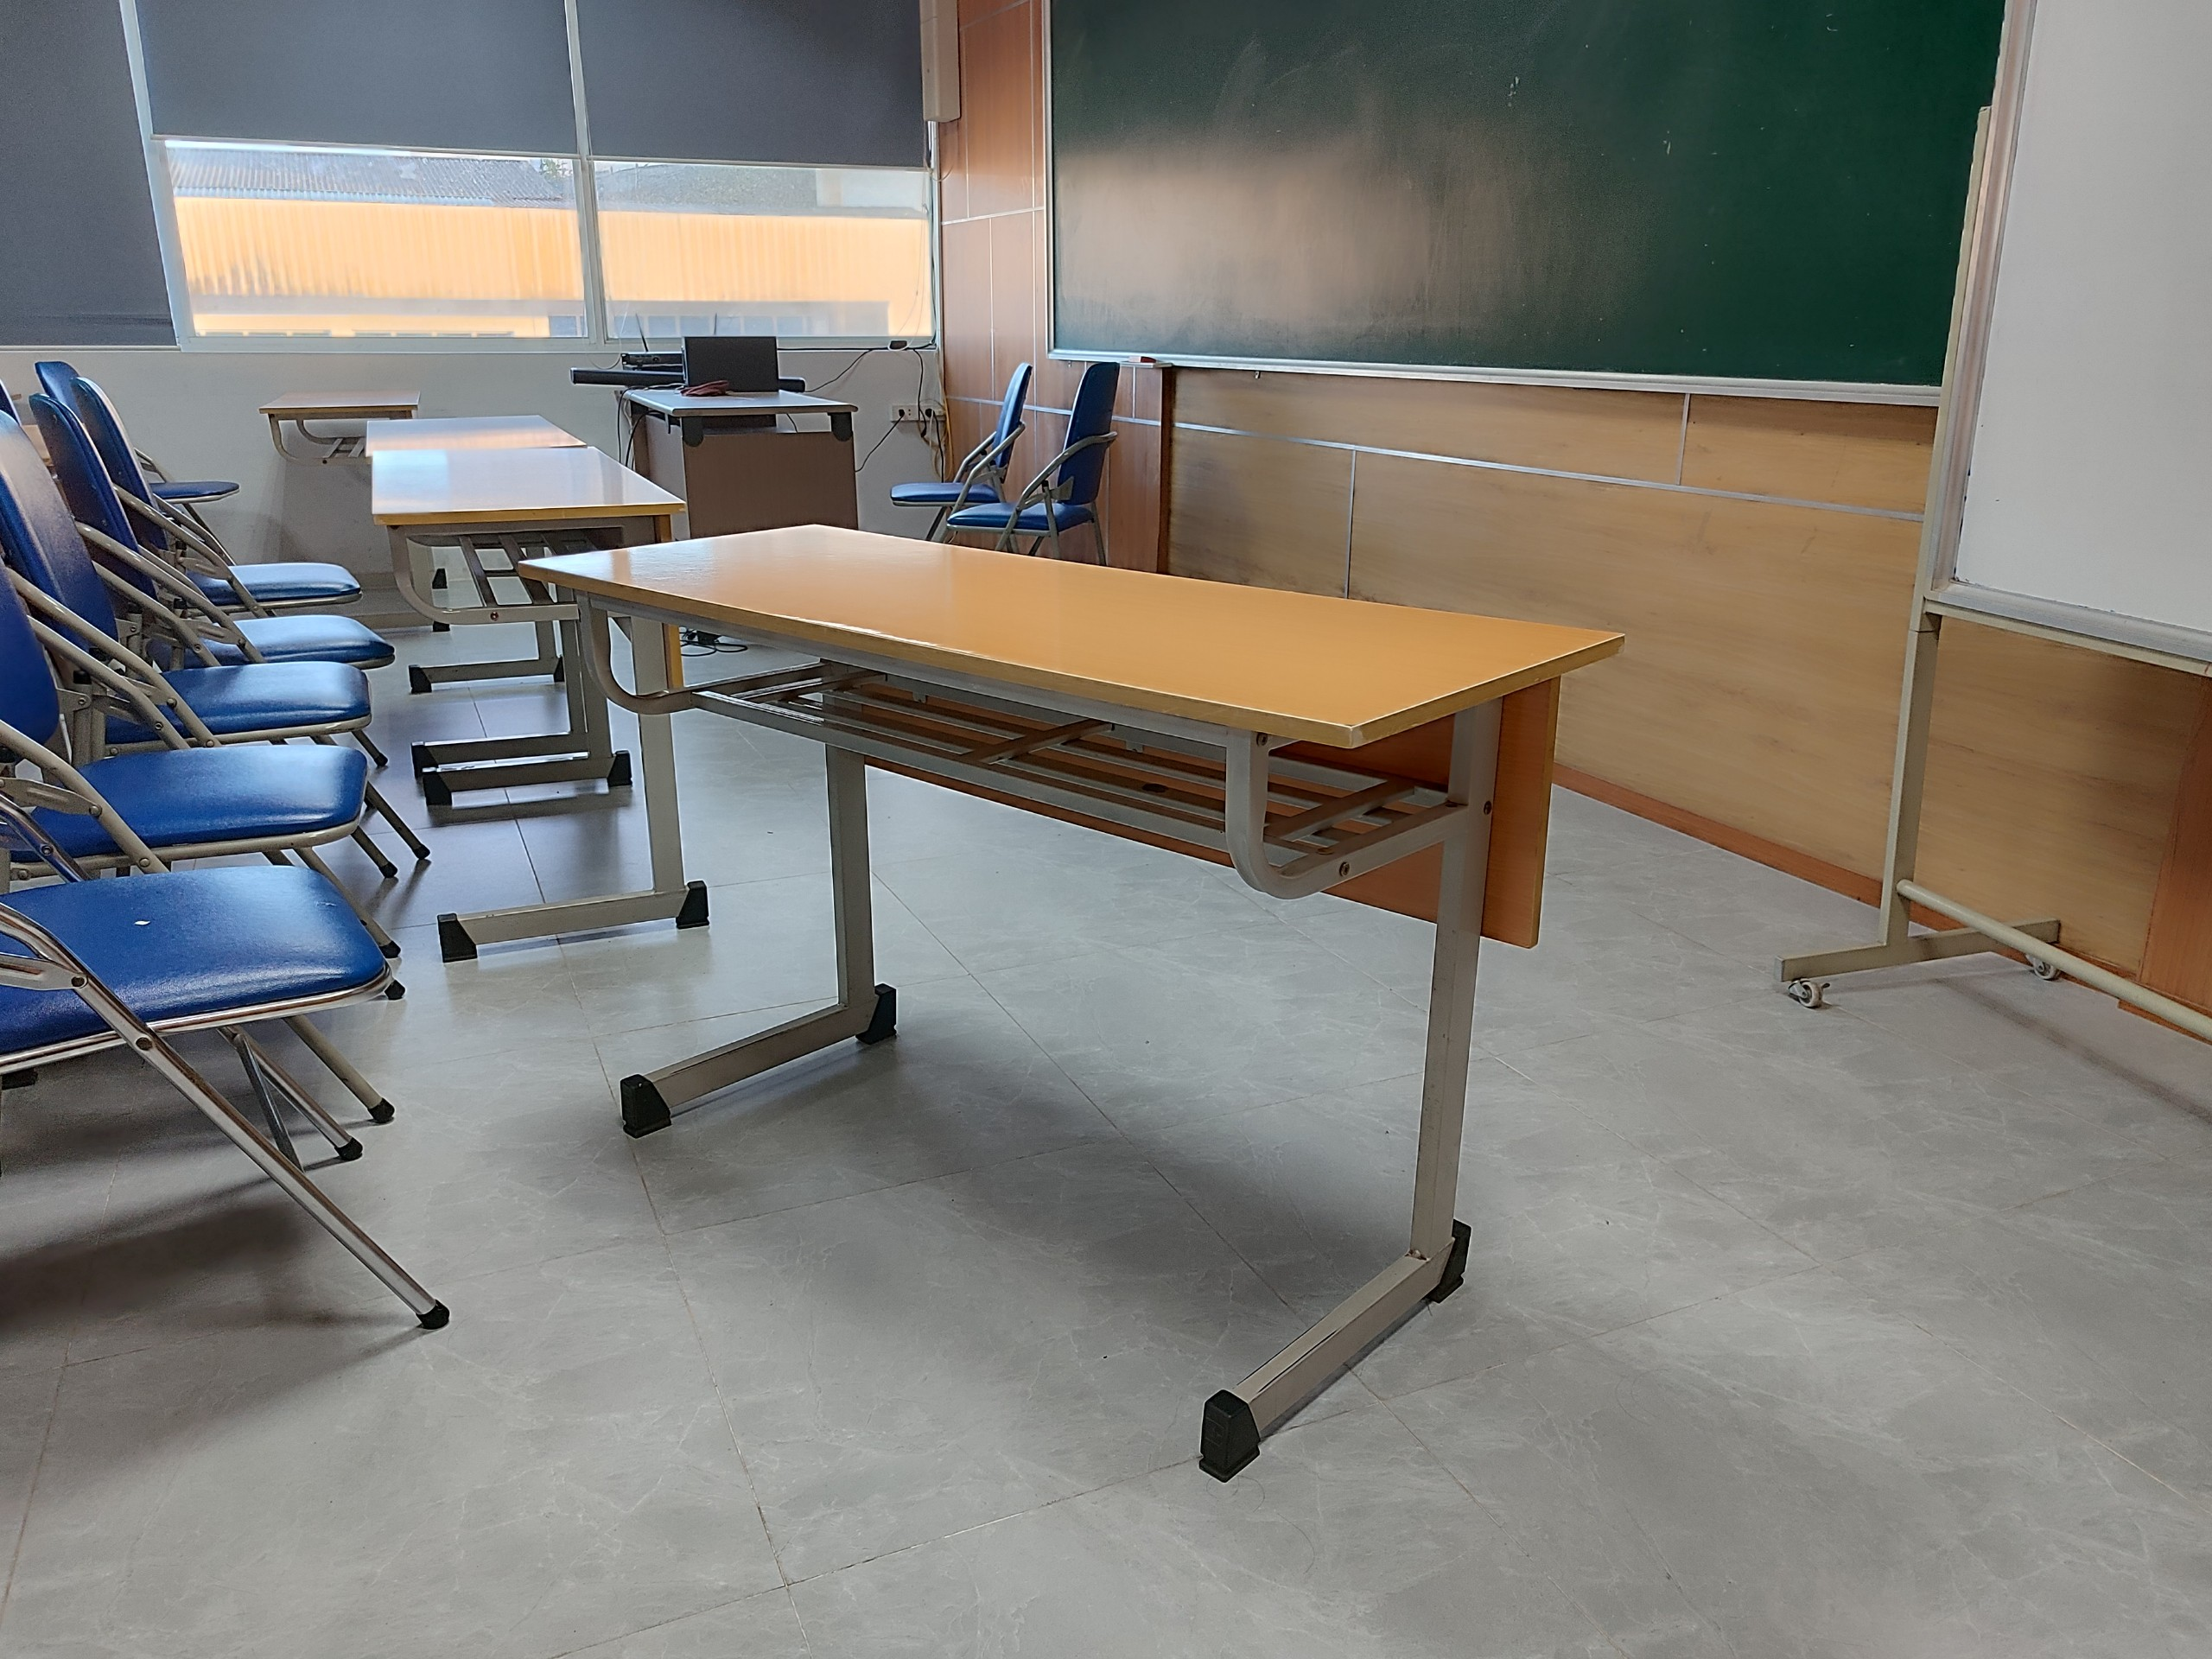
\includegraphics[width=0.49\textwidth]{go2.jpg}
    \caption{Wood Table with Comparison.}
\end{figure}

\subsection{Gameplay Design}
\subsubsection{The Main Menu}
\hspace*{1.5em} When the game is opened, the main menu will be the first thing to be seen.
Along with the features of the game displayed in the main menu, the player will also be seen at the top left corner of the screen. And all of the model features that were mentioned before are all here, including the Body Center Dot, the Upper Body Landmark Tracker, and the Hand Center Dot.\\

With this Main Menu scene, the player can use their hand to control the in-game cursor, which is the red square floating around the screen.
Then, in the background of the Main menu, the in-game player is running endlessly through the hallways.
There are 4 options in this first screen: "Start", "Modes", "Shop" and "Quit". To choose any button, use the hand to hover to cursor over the one that is wanted.\\

\begin{figure}[ht]
    \centering
    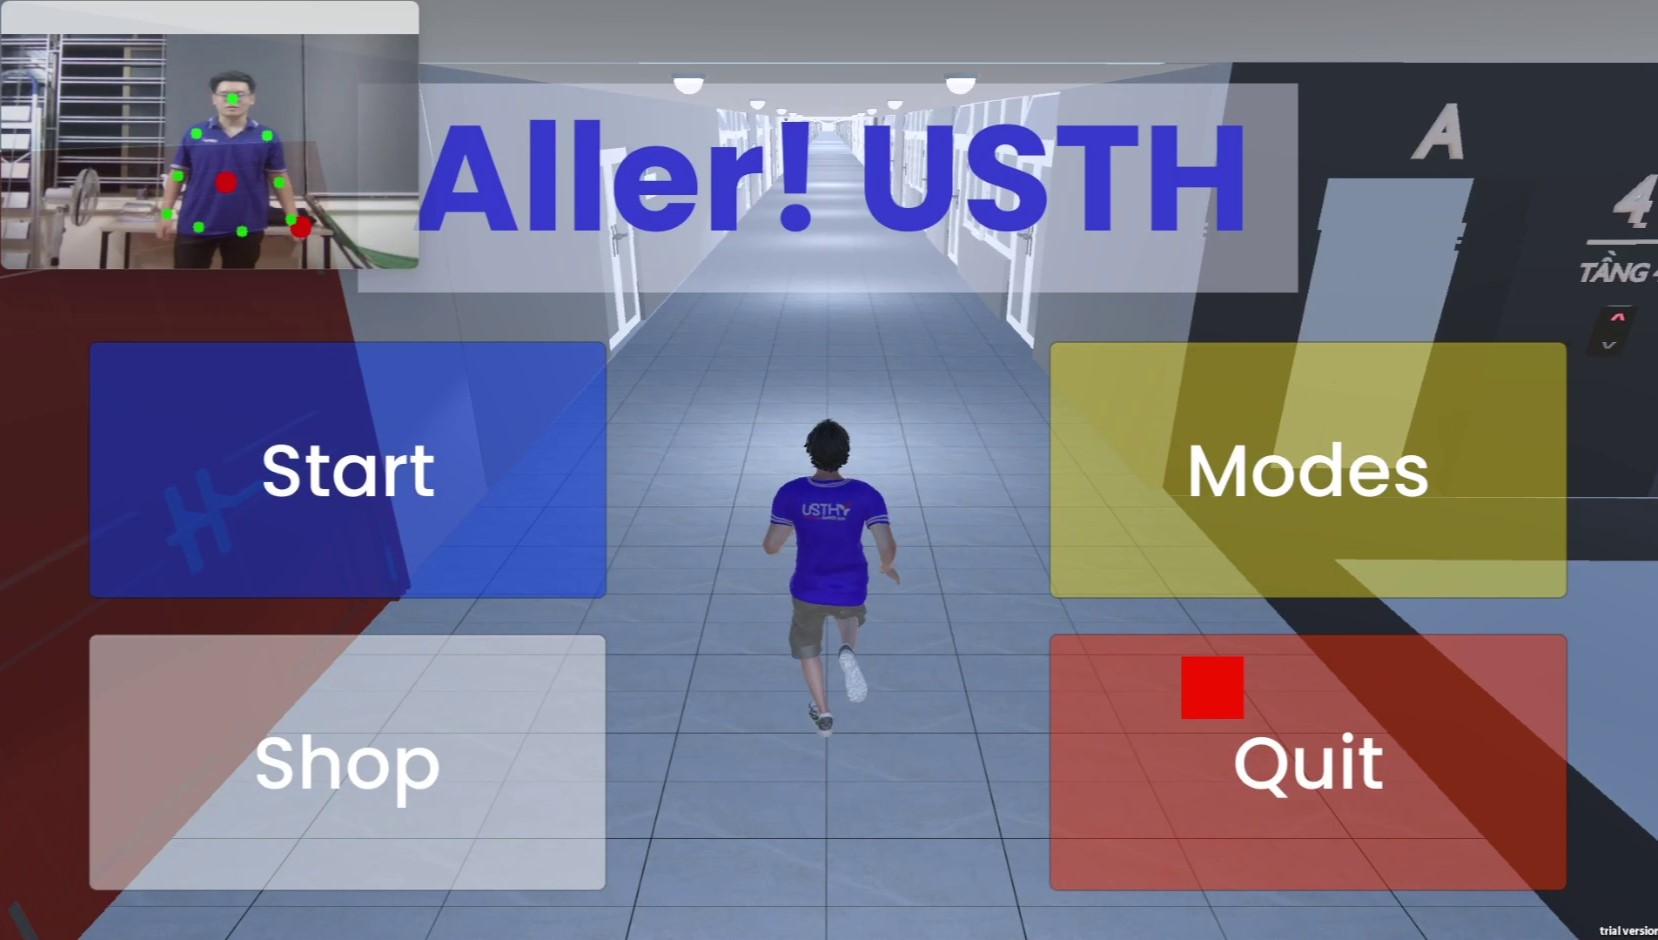
\includegraphics[width=0.7\textwidth]{game1.jpg}
    \caption{Main Menu Screen.}
\end{figure}

\subsubsection{Endless-Running Game Mode}
\hspace*{1.5em} When pressed Start at the Main menu, the player will enter the main game mode: Endless-Running. 
The objective of the game is to run as far as possible, to gain as much score as possible. 
But be careful, because on the way there will be objects placed randomly to make the player fall over and end the run.\\

The score of the game is tracked by the position of the player compares to where they started. The further the player go, the higher the score they earned.
But if the player touch any obstacles along the way, the score run will stop and the Game Over screen will pop-up to end the game.\\

To get through the obstacles, the player has to dodge them by move to the left, right, run over the obstacles or even roll/slide under them.
And to do those actions, this mode uses the dot and the threshold in the Body Center Tracking, so if the player's body center get through the threshold line, the game character will do the same action.\\

The coins are also obtainable so that they player can buy other models in the Shop. And there are a High Score system also.
Both of them are stored in the player's data directory PlayerPrefs, so they will be tracked when the player leaves the game.\\

The hallways and the lanes with obstacles work just like the Main Menu where they spawn infinitely until the game is over and randomly so that the game is not get boringly looped.

\begin{figure}[H]
    \centering
    \includegraphics[width=0.49\textwidth]{game2.jpg}
    \includegraphics[width=0.49\textwidth]{game4.jpg}
    \includegraphics[width=0.49\textwidth]{game5.jpg}
    \includegraphics[width=0.49\textwidth]{game6.jpg}
    \includegraphics[width=0.49\textwidth]{game7.jpg}
    \caption{Endless-Running Gameplay.}
\end{figure}

And when the Game Over screen is triggered, the player can turn back to using their hand to control the cursor to choose options.

\begin{figure}[H]
    \centering
    \includegraphics[width=0.65\textwidth]{game8.jpg}
    \caption{Game Over Screen.}
\end{figure}

\subsubsection{Object-Slicing Game Mode}
\hspace*{1.5em} If lucky in the main game, the player has the chance to meet a fruit portal on the way which lead to this game mode: Object-Slicing Game Mode (Inspired by Fruit Ninja).\\

The background is from one of the hallways, and the sign said "Laboratory For Materials Characterization" but the time constraint to work on these models is limited so I took the Fruit design tutorial online and made it here.\\

The Fruit Slicer (Blade) uses the Hand Center Tracker as the cursor to follow along. So the player will use the movement of the hand to control the cursor moving around the screen, touch the fruit to score points and avoid hitting the bomb.\\

Each fruit has a different collider shape, with some really big like a watermelon but end up giving less points, and some really small like a pear or an apple, but more rewarding when sliced through.\\

Occasionally, some bomb will appear to distract the player, and if hit, the player will be sent back to the main game Endless Running game mode, and the total score will be added there also.

\begin{figure}[h]
    \centering
    \includegraphics[width=0.85\textwidth]{game3.jpg}
    \caption{Object-Slicing Gameplay.}
\end{figure}

\clearpage
\subsubsection{Shape-Fitting Game Mode}
\hspace*{1.5em} If lucky in the main game, the player has the chance to meet a hole portal on the way which lead to this game mode: Shape-Fitting Game Mode (Inspired by Hole in the Walls).\\

In the same hallway, there are walls that are incoming, and the objective is to pass as many wall as the player can without touching any of them.\\

This game mode uses the Upper Body tracker, so the model made from the lines and dots on the screen can be control by the player moving in real life.\\

Only the Upper Body be tracked in the game mode because hardly people can move away from the camera enough so that it could track their knees and feet without making it too hard for the player to see the actural screen.
And also the model in Blender is not attracted to this game character because the game mechanic to add landmarks to the rigged animation is weird and somehow does not support this for some reason.\\

The game design is simple: Get through the shape in the wall, earn point; touch the wall, game over and get back to the main Endless-Running game mode. And the walls will move faster and spawn quicker the more walls the player get through, to level up the difficulty.\\

\begin{figure}[h]
    \centering
    \includegraphics[width=0.85\textwidth]{game13.jpg}
    \caption{Shape-Fitting Gameplay.}
\end{figure}

\clearpage
\subsubsection{Other Game Aspects}
\hspace*{1.5em} If the player does not want to play multiple game in one like that, they can control the cursor by their hand in the Main Menu screen and chooses Modes instead of Start. In that way, the Modes screen will appear with these choices.\\

The Endless-Running Mode will still send the player to the Endless-Running game, but this time no more Portal will spawned so that they can peacefully run in this mode. The Highscore System will be different for this, but the Coins will still add up.\\

The Fruit-Slicing Mode and the Shape-Fitting Mode will be the same, you will start the game mode as soon as you hover the button. And when the Game Over screen is triggered when the player hits the bomb or touches the wall, it will have the Game Over screen like at the end of the Endless-Running mode.
\begin{figure}[h]
    \centering
    \includegraphics[width=0.49\textwidth]{game11.jpg}
    \includegraphics[width=0.49\textwidth]{game12.jpg}
    \caption{Choose Game Mode.}
\end{figure}

The Shop scene will appear when hover on the Shop button on the Main menu or on the Game Over screen.\\

The shop also make use of the Hand Center tracker as the cursor. Unfortunately, the Shop screen is not really finished yet, so here is a glimpse of Shop content.

\begin{figure}[h]
    \centering
    \includegraphics[width=0.49\textwidth]{game9.jpg}
    \includegraphics[width=0.49\textwidth]{game10.jpg}
    \caption{Shop Screen.}
\end{figure}


\clearpage

\section{TESTING / EXPERIMENTAL VALIDATION}
\subsection{Experimental Validation}

This section presents the experimental validation for the Aller! USTH game, focusing on the effectiveness and responsiveness of two major pose detection technologies: MediaPipe Pose and MoveNet. The results are crucial in understanding how these technologies perform under different environmental settings, which directly impacts the game's responsiveness and user experience.

\subsubsection{Distance Sensitivity Analysis}

These tables compare the performance of the two technologies in terms of their ability to detect movements at various distances. The 'Unable to detect' row indicates the distances at which each technology fails to detect the player, while 'Unstable detection' highlights ranges where detection is possible but not consistently reliable.

\begin{table}[h]
    \centering
    \caption{Distance Sensitivity Analysis for Aller! USTH.}
    \begin{tabular}{|c|c|c|}
        \hline
        \textbf{Condition} & \textbf{MediaPipe Pose} & \textbf{MoveNet} \\
        \hline
        \multicolumn{3}{|c|}{\textbf{0.26m Camera Height, 110°-120° Laptop Lid}} \\
        \hline
        Unable to detect   & $<$0.52m or $>$21.3m & $<$0.48m or $>$18.6m \\
        \hline
        Unstable detection & 0.52m-0.7m or 20.6m-21.3m & 0.48m-0.84m or 17.9m-18.6m \\
        \hline
        \multicolumn{3}{|c|}{\textbf{0.75m Camera Height, 90°-95° Laptop Lid}} \\
        \hline
        Unable to detect   & $<$0.42m or $>$21.3m & $<$0.36m or $>$18.6m \\
        \hline
        Unstable detection & 0.42m-0.5m or 20.6m-21.3m & 0.36m-0.68m or 17.9m-18.6m \\
        \hline
    \end{tabular}
\end{table}

\subsubsection{Response Time Evaluation}

This table provides insights into the latency involved in detecting specific movements, which is fundamental for real-time interaction in the Aller! USTH game. Shorter response times are indicative of a more fluid and responsive gaming experience.\\

\textbf{Computer configurations used for the response time evaluation:}\\ 
\begin{table}[h]
    \begin{tabular}{lll}
    \textbf{Laptop 1:}                                                                                                                                            & \textbf{Laptop 2:}                                                                                                                                               & \textbf{PC:}                                                                                                                                                  \\
    \begin{tabular}[c]{@{}l@{}}- RAM: 4GB\\ - Storage: 8192 MB\\ - GPU: Intel(R) HD Graphics 620\\ - Resolution: 1366x768\\ - Refresh rate: 60.02 Hz\end{tabular} & \begin{tabular}[c]{@{}l@{}}- RAM: 8GB\\ - Storage: 16384 MB\\ - GPU: Intel(R) UHD Graphics 630\\ - Resolution: 1920x1080\\ - Refresh rate: 60.02 Hz\end{tabular} & \begin{tabular}[c]{@{}l@{}}- RAM: 24GB\\ - Storage: 32768 MB\\ - GPU: NVIDIA GeForce RTX 3080\\ - Resolution: 2560x1440\\ - Refresh rate: 144 Hz\end{tabular}
    \end{tabular}
\end{table}

\clearpage

\begin{figure}[h!]
    \centering
    \begin{subfigure}{0.49\textwidth}
        \centering
        \caption{Laptop 1}
        \begin{tabular}{|c|c|c|}
            \hline
            & MediaPipe Pose & MoveNet \\
            \hline
            Time to boot & 15.2s & 12.2s \\
            \hline
            Left & 0.83s & 0.68s \\
            \hline
            Right & 0.84s & 0.68s \\
            \hline
            Jump & 0.5s & 0.45s \\
            \hline
            Crouch & 0.55s & 0.4s \\
            \hline
        \end{tabular}
    \end{subfigure}
    \begin{subfigure}{0.49\textwidth}
        \centering
        \caption{Laptop 2}
        \begin{tabular}{|c|c|c|}
            \hline
            & MediaPipe Pose & MoveNet \\
            \hline
            Time to boot & 13.2s & 8.4s \\
            \hline
            Left & 0.8s & 0.6s \\
            \hline
            Right & 0.8s & 0.6s \\
            \hline
            Jump & 0.45s & 0.38s \\
            \hline
            Crouch & 0.45s & 0.35s \\
            \hline
        \end{tabular}
    \end{subfigure}
    \begin{subfigure}{0.6\textwidth}
        \centering
        \caption{PC}
        \begin{tabular}{|c|c|c|}
            \hline
            & MediaPipe Pose & MoveNet \\
            \hline
            Time to boot & 9.21s & 7.4s \\
            \hline
            Left & 0.67s & 0.4s \\
            \hline
            Right & 0.72s & 0.42s \\
            \hline
            Jump & 0.4s & 0.38s \\
            \hline
            Crouch & 0.38s & 0.34s \\
            \hline
        \end{tabular}
    \end{subfigure}
    \caption{Response Time Evaluation for MediaPipe Pose and MoveNet using CPU.}
\end{figure}

\subsubsection{Caloric Evaluation}

Our product is designed with a dual purpose: to make exercise enjoyable through engaging gameplay while also delivering tangible health benefits, particularly in terms of calorie burning. This balance is essential for the real-world relevance and success of our product.\\

\textbf{Methodology}\\
Our method to measure the game's effectiveness was straightforward yet thorough. We played the game for 1.5 minutes at a time, repeating this 20 times to simulate a 30-minute exercise session. During each game, we carefully noted the number of specific movements - such as moving left or right, jumping, and crouching. This data was then averaged to provide a clear picture of physical activity within a typical game session, as shown in Table below.

\begin{table}[h]
    \centering
    \caption{Number of Movements in certain period of playtime.}
    \begin{tabular}{|c|c|c|c|c|c|}
        \hline
                          & Left & Right & Jump & Crouch & Estimated play time \\
        \hline
        Average in 1 game & 26   & 26.8  & 6.6  & 12     & 1.5 minutes         \\
        \hline
        Total in 20 games & 520  & 536   & 132  & 240    & 30 minutes          \\
        \hline
    \end{tabular}
\end{table}

\textbf{Calorie Burning Analysis:}\\
We estimated the calorie burn of these movements by comparing them with similar real-life exercises. For instance, we likened in-game side movements to steps, jumping to skipping rope, and crouching to doing squats. The calorie count for each action was calculated based on these comparisons:\\[5pt]
- Side movements: About 0.05 to 0.1 calories each \cite{baum2018}.\\
- Jumping: Similar to skipping rope, burning roughly 0.11 calories per jump \cite{frey2015}.\\
- Crouching: Comparable to doing a squat, with about 0.32 calories burned each time \cite{english2022}.\\

\textbf{Comparison with Traditional Exercises:}\\
To further validate our game's fitness benefits, we compared its calorie-burning capacity with common exercises like jogging, running, and swimming over the same duration of 30 minutes \cite{vinmec2019} \cite{harvard2004}. This comparison is detailed in Table below and shows how our game stacks up against more traditional forms of exercise.\\

\begin{table}[h]
    \centering
    \caption{Calorie-burning Exercises Comparison of an average person (70kg) in 30 minutes.}
    \begin{tabularx}{\textwidth}{|Y|Y|Y|Y|Y|Y|}
        \hline
        & Aller! USTH & Jogging (at 6.5Km/h) & Calisthenics (moderate) & Running (at 8Km/h) & Swimming (casual) \\
        \hline
        Calories Burned & 170.5 Kcal & 175 Kcal & 162 Kcal & 288 Kcal & 246 Kcal \\
        \hline
    \end{tabularx}
\end{table}
\clearpage

\subsection{Beta-Testing Evaluation}
So in order to test the game we decided to ask some of my friends or family to help me and according to their experience give a rating from 1 to 10 for multiple aspect of the game.

\subsubsection{Beta Testing Process}
\hspace*{1.5em}Aller! USTH was packaged and can be downloaded at this GitHub repository. 
About 30 friends and family members were invited to try out the game, and after three days, feedback started rolling in from those who gave it a shot.\\

A survey form in Google Docs was included with the game download, and here's what was found out. Out of the 30 people asked, 5 took the time to send their feedback back. 
Not surprisingly, none of them were from USTH - students there are probably busy with their thesis right now and wouldn't have had the time to provide feedback.\\

\begin{figure}[ht]
    \centering
    \includegraphics[width=0.35\textwidth]{survey1.png}
    \includegraphics[width=0.35\textwidth]{survey2.png}
    \includegraphics[width=0.35\textwidth]{survey3.png}
    \caption{Survey Screenshots.}
\end{figure}

\begin{table}[]
    \center
    \caption{Beta-Testing Evaluation Responses}
    \begin{tabular}{|c|c|c|c|c|}
    \hline
    \rowcolor[HTML]{C0C0C0} 
    \textbf{User} & \textbf{Overall Experience} & \textbf{Endless-Running} & \textbf{Fruit-Slicing} & \textbf{Shape-Fitting} \\ \hline
    User 1        & 8                           & 8                        & 8                      & 5                      \\ \hline
    User 2        & 5                           & 6                        & 5                      & 2                      \\ \hline
    User 3        & 8                           & 9                        & 9                      & 7                      \\ \hline
    User 4        & 8                           & 9                        & 8                      & 8                      \\ \hline
    User 5        & 7                           & 7                        & 6                      & 5                      \\ \hline
    \end{tabular}
\end{table}

\begin{table}[]
    \center
    \begin{tabular}{|c|c|c|c|c|c|}
    \hline
    \rowcolor[HTML]{C0C0C0} 
    \textbf{User} & \textbf{Latency} & \textbf{Graphics} & \textbf{Difficulty} & \textbf{Long-term Playability} & \textbf{Recommend Rate} \\ \hline
    User 1        & 4                & 7                 & 4                   & 4                                                                        & 4                                                                 \\ \hline
    User 2        & 7                & 8                 & 2                   & 2                                                                        & 5                                                                 \\ \hline
    User 3        & 6                & 10                & 2                   & 7                                                                        & 8                                                                 \\ \hline
    User 4        & 9                & 10                & 1                   & 7                                                                        & 7                                                                 \\ \hline
    User 5        & 6                & 7                 & 5                   & 6                                                                        & 5                                                                 \\ \hline
    \end{tabular}
\end{table}

\subsubsection{Game Experience}
\hspace*{1.5em} In general, the testers' game experience is not too bad. The scores varies, but mostly they are above average so it counts as good enough.\\

The game experience received varied ratings from the beta tester. The scores for the game overall are mostly 8, giving a generally positive vibe but with room for improvement.
The highest rated game mode among the three is Endless-Running, the main game mode with two 9 marks and an 8, follow up with Fruit-Slicing and lastly Shape-Fitting which the scoring are mostly under average.\\

Although the game is doing great in these tester's survey answer, they are mostly familiar with the game since they kept up with the game development from the very start. So this survey might be bias and the game needed another survey where the is no bias and survey varieties of people to check out the game and give honest opinion.

\subsubsection{Other Aspects}
\hspace*{1.5em}The survey also asked the testers questions other than the prue gameplay experience.\\

In the Latency criteria, the results are mixed, with User 1 put a 4, User 4 put a 9 and many in-between. This might be because of the machine that they used to run the game, which might varies from old company laptop with weak comparability to run the model and the game all at once, to huge modern pc with good CPU and all.\\

In the Graphic rating, the game deserved to be scored that high by the testers, considering that was the most time-comsuming part of the project.
The game is quite easy in their option, where the Game Difficulty criteria has a really low score, so in the future the difficulty of each game mode will be increase to make it as interesting and engaging as possible.\\

Finally, although the game's long-term playability is not high, most of the testers do willing to recommend the game to others, which is good for the future as more people will know and have access to the game and give more valuable opinion.\\
\hspace*{1.5em}

\clearpage
\section{SUMMARY}
\subsection{Conclusion}
\hspace*{1.5em}This thesis successfully developed "Aller! USTH," a video game that effectively integrates physical activity into gameplay using human pose estimation technology. The game, inspired by popular titles like Subway Surfers and Fruit Ninja, encourages players to perform specific physical movements to progress, addressing the pressing issue of sedentary behavior among gamers, particularly within the University of Science and Technology of Hanoi (USTH).\\

The project utilized two leading pose estimation models, MediaPipe Pose and MoveNet, and evaluated their performance using the COCO-WholeBody dataset and a custom dataset created from friends' landmarks data. The evaluation revealed that both models exhibited high accuracy in keypoint detection, with MediaPipe Pose demonstrating a slightly higher frame rate and lower processing time.\\

The game design incorporated a Python-Unity communication system, enabling real-time interaction between the pose estimation model and the game engine. This allowed for dynamic gameplay where player movements directly influenced the game's progression. The game features three distinct game modes: endless-running, object-slicing, and shape-fitting, each requiring different physical actions from the player.\\

Experimental validation, including distance sensitivity analysis, response time evaluation, and caloric evaluation, confirmed the game's effectiveness in promoting physical activity. Beta testing provided valuable feedback on the game's experience and user interface, further refining the game's development.\\

"Aller! USTH" demonstrates the potential of integrating physical activity into gaming experiences, promoting a healthier lifestyle for gamers. The project's success lays the groundwork for future research and development of active gaming solutions, contributing to the growing body of research on the health benefits of active gaming.
\clearpage
\subsection{Future Development}
\hspace*{1.5em}While "Aller! USTH" showcases the potential of incorporating physical activity into gaming, there are several avenues for future development to enhance its impact and expand its reach:\\

- \textbf{Finish Shop Function:} Implementing a fully functional in-game shop would allow players to purchase virtual items, such as character customizations, power-ups, or new game modes. This could incentivize players to continue playing and engaging with the game.\\

- \textbf{Improve the Shape-Fitting Game Mode:} Further refining the Shape-Fitting game mode could enhance its complexity and engagement. This could involve introducing more challenging shapes, incorporating dynamic elements, or adding a scoring system based on accuracy and speed.\\

- \textbf{Reduce Latency:} Optimizing the communication system between the pose estimation model and the game engine could significantly reduce latency, making the gameplay more responsive and immersive. This could involve exploring more efficient communication protocols, optimizing code for performance, or leveraging cloud-based processing.\\

- \textbf{Experiment with Other Pose Estimation Models:} Exploring alternative pose estimation models beyond MediaPipe Pose and MoveNet could lead to improved accuracy, efficiency, or specialized features. Evaluating the performance of newer models or models optimized for specific tasks could further enhance the game's responsiveness and user experience.\\

- \textbf{Multiplayer Mode:} Adding a multiplayer mode would allow players to compete or collaborate with friends, fostering social interaction and increasing engagement. This could involve real-time gameplay where players' movements are synchronized, or asynchronous challenges where players compete against each other's scores.\\
\clearpage

\addcontentsline{toc}{section}{REFERENCES}
\bibliography{references}

\end{document}
